\documentclass[12pt, a4paper,twoside]{tesi_upf}

%CODIFICACIÓ
%\usepackage[latin1]{inputenc}

%DIAGRAMA DE GANTT
\usepackage{pgfgantt}

%IDIOMES
\usepackage[catalan,english]{babel}

%PER A INCLOURE GRÀFICS I EL LOGO DE LA UPF
\usepackage{graphicx}
\usepackage{caption}
\usepackage{acronym}
\usepackage{multirow}
%FONTS TIMES O GARAMOND, 
\usepackage{times}
%\usepackage{garamond}
\usepackage{url}

\usepackage{pdfpages}
%SENSE HEADINGS: NO MODIFICAR
\pagestyle{plain}

%PER A L'ÍNDEX DE MATÈRIES
\usepackage{makeidx}
\makeindex

%ESTIL DE BIBLIOGRAFIA
%\bibliographystyle{apalike}

%AQUEST DOCUMENT ÉS EN ANGLÈS
\selectlanguage{english}

%AFEGIU EN AQUESTA PART LES VOSTRES DADES
\title{Aerial sensor platform}
\author{Gonzalo Hermida Ruiz}
\thyear{2014}
\department{Departament de Tecnologies de la Informació i les Comunicacions (DTIC)}
\supervisor{Jaume Barceló, Carles Ayesa, Luis Sanabria}

\begin{document}

\frontmatter

\maketitle

\cleardoublepage

%%%%%% Dedicatòria; si no es vol posar, comenteu fins a final de dedicatòria

\noindent To my family.

\cleardoublepage

%%%%%% Final de dedicatòria

%%%%%% Agraïments; si no es vol posar, comenteu fins a final de agraïments
\noindent {\Large \sffamily Acknowledgments}
\\[12pt] 
        
I would like to thank to 
\\[8pt]

Also, to 
\\[8pt]

At last, 

\cleardoublepage

%%%%%% Final dels agraïments

%ABSTRACT EN DOS IDIOMES. COM A MÍNIM CATALÀ. SI L'ALTRE ÉS EN CASTELLA CANVIEU EL QUE POSA ABSTRACT
\selectlanguage{english}
\section*{\Large \sffamily Abstract}

This  work  addresses  the  gathering  of  data  in  areas  of  difficult  access  or  which  are potentially dangerous. Examples include high tension power lines, collapsed buildings and fire areas. We build a flying platform with the ability of carrying light sensors (e.g., small cameras or infrared cameras) and transmit the sensed data wirelessly to a control point. The platform is a highly manoeuvrable multicopter that uses the Arduino microcontroller and the multiwii software.

\selectlanguage{catalan}
\vspace*{\fill}
\section*{\Large \sffamily  Resum}

Abtracte en català

\vspace*{\fill}

\selectlanguage{english}
\cleardoublepage
%FIN DE ABSTRACTE

%PREFACI OPCIONAL. SI NO ES VOL, COMENTEU FINS EL FINAL DE PREFACI
%{\bf Prefaci}
%
%\cleardoublepage
%FINAL DE PREFACI


%TAULA DE CONTINGUTS: OBLIGATÒRIA
\tableofcontents

%INDEX DE FIGURES; NOMÉS ES POSA SI HI HA FIGURES
\listoffigures
%Fa que aparegui al sumari
\addcontentsline{toc}{chapter}{List of figures}

%INDEX DE TAULES; NOMÉS ES POSA SI HI HA TAULES
\listoftables
%Fa que aparegui al sumari
\addcontentsline{toc}{chapter}{List of tables}

%INDEX DE ACRONIMS
\cleardoublepage
\thispagestyle{empty}
\addcontentsline{toc}{chapter}{List of Abbreviations}
\vspace*{1.95cm} \hspace*{-0.155cm} %,88
\textbf{{\huge \sffamily List of Abbreviations}\\}
\vspace*{0.5cm}         
\begin{acronym}
%\acro{AP}{Access Point}
%\acro{BMX6}{BatMan-eXperimental version 6}
%\acro{BSS}{Basic Service Set}
\end{acronym}

%COMENÇA EL TEXT
\mainmatter
\chapter{Introduction}

This thesis consist on the construction of an ardupilot in order to the gathering of data in areas of difficult access due to the ability of carrying light sensors and transmit the sensed data wirelessly to a control point. An ardupilot is a remotely controlled UAV (Unmanned Aerial Vehicle)  based on Arduino, a free hardware platform based on a board with a microcontroller and a development environment, and MultiWii, a free software used to control multirotor RC models. 
\\[12pt]

An Arduino board consists on a microcontroller with complementary components to facilitate programming and incorporation into other circuits. An important aspect of the Arduino is the standard way that connectors are exposed, allowing the CPU board to be connected to a variety of interchangeable add-on modules known as shields, which are printed circuit expansion boards that plug into the normally supplied Arduino pin-headers providing i.e. motor controls or GPS.
\\[12pt]

The Arduino integrated development environment (IDE) is a cross-platform application written in Java, and is derived from the IDE for the Processing programming language and the Wiring projects. The Arduino IDE uses the GNU toolchain and AVR Libc to compile programs, and uses avrdude to upload programs to the board. Arduino programs are written in C or C++ and called "sketch". 
\\[12pt]

The MultiWii is an open source software project aiming to provide the brain of a RC controlled multi rotor flying platform. It is compatible with several hardware boards and sensors and have a lot of supported features.
\\[12pt]

\chapter{Mounting the device}

This section details step by step how to assembly the device, with the addition of several reviews, tips and images to provide an explanation as accurate and understandable as possible.

\section{Mounting the arms structure}

The motors must be screwed onto the ends of the arms. The screws that brought the motors were too short, so had to buy some longer.

\noindent%
\begin{minipage}{\linewidth}
\vspace{10 mm}
\makebox[\linewidth]{%
  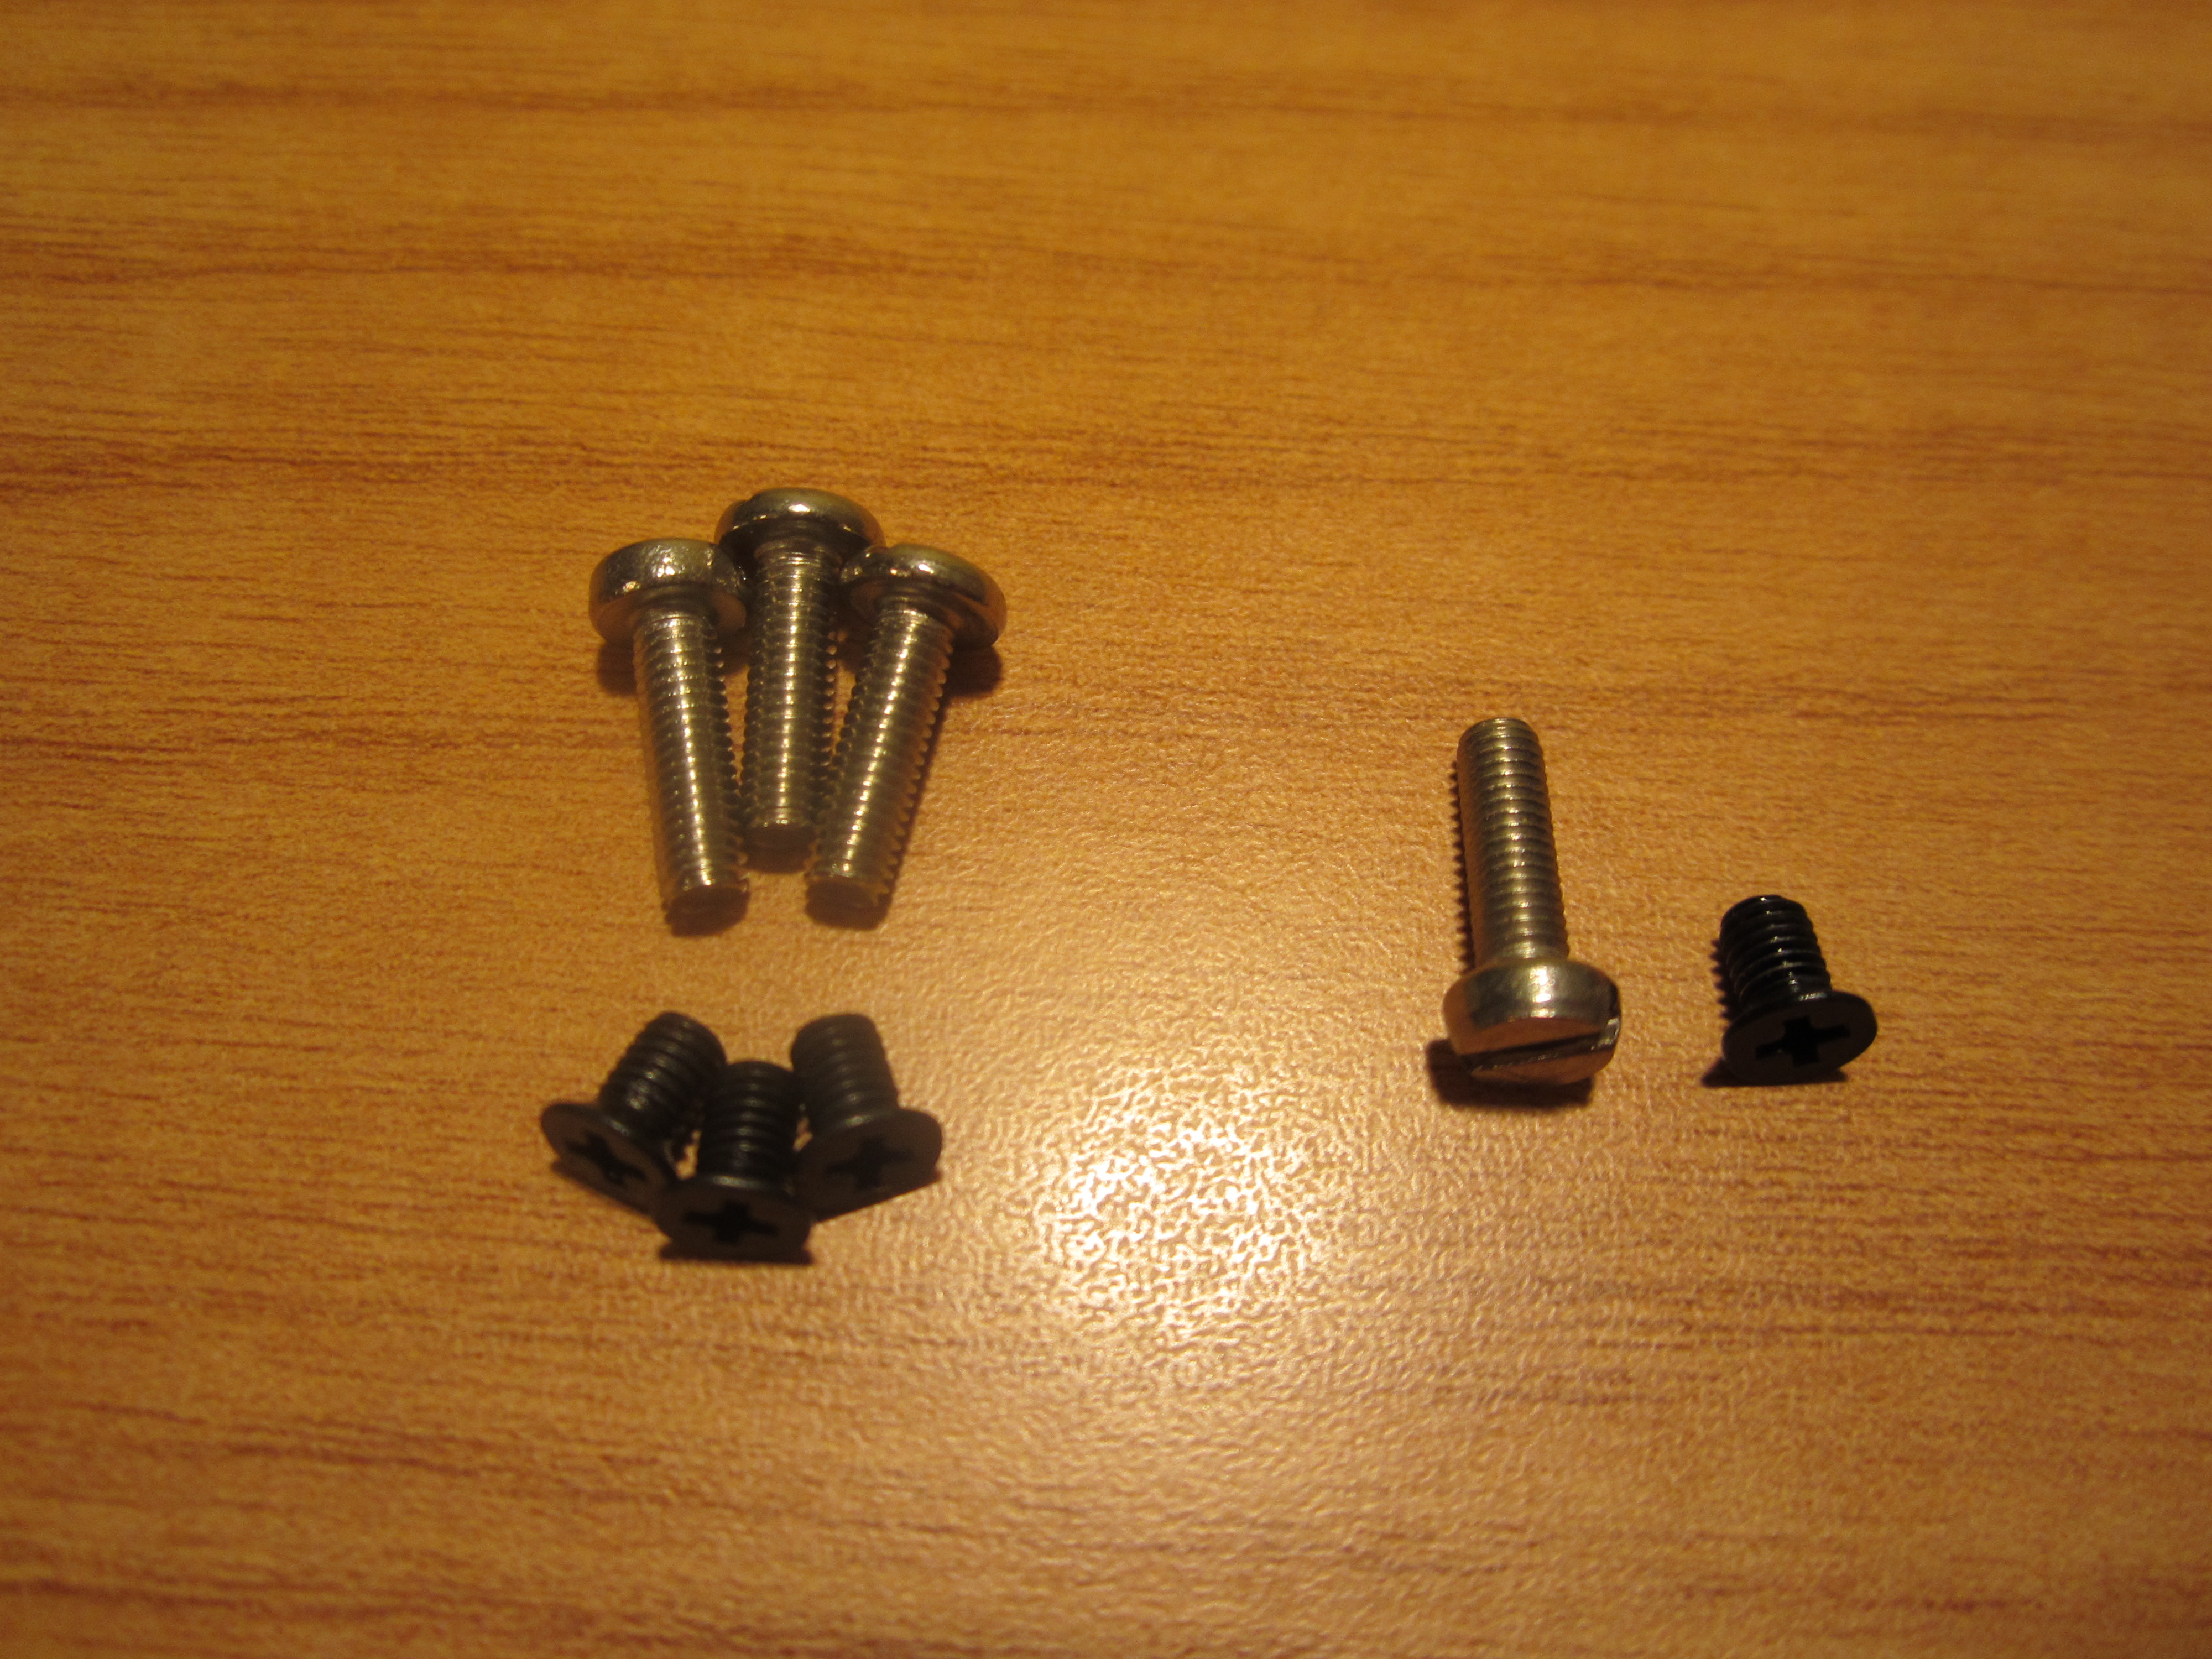
\includegraphics[width=0.8 \linewidth]{Images/Mounting/IMG_0342.jpg}}
\captionof{figure}{}% only if needed
\label{screwDifferences}
\end{minipage}    
\clearpage

We should note that the holes motors and arms are not equally spaced, so it is possible that when we screw a couple of screws fit and the rest not. To make sure they fit correctly, you must make the motor cables face the other end of the arm as you see in the figure below.

\noindent%
\begin{minipage}{\linewidth}
\vspace{10 mm}
\makebox[\linewidth]{%
  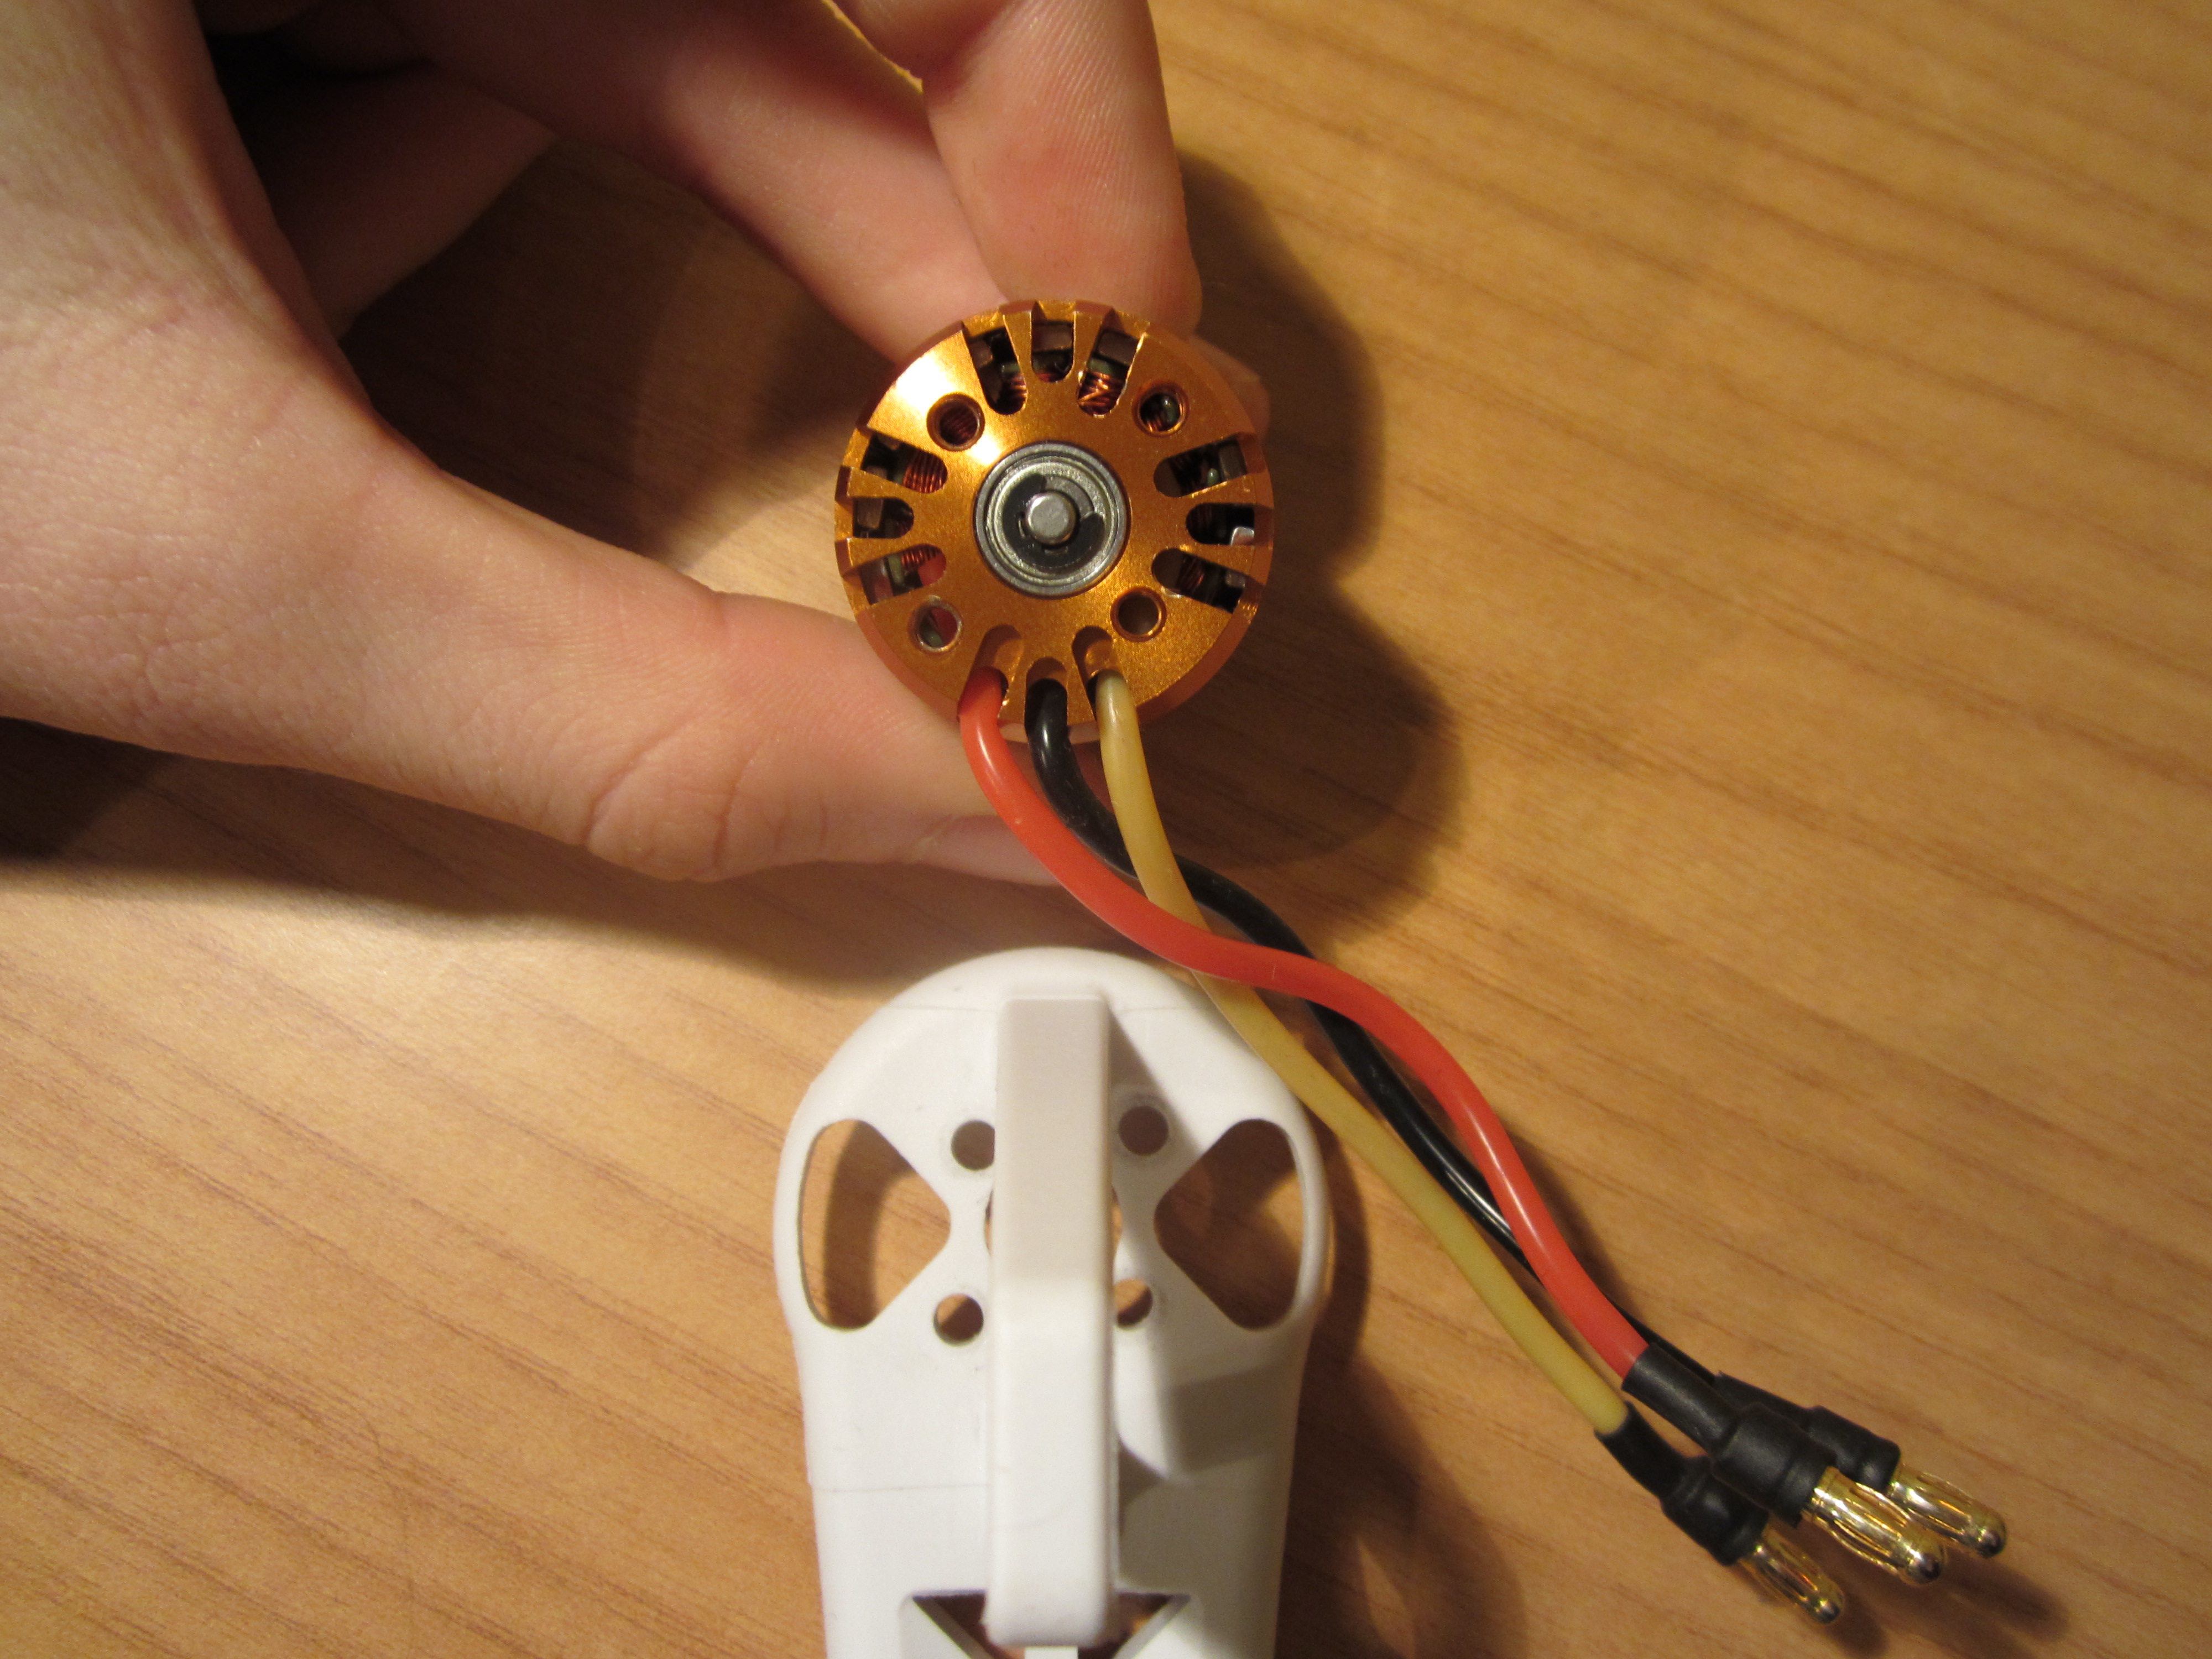
\includegraphics[width=0.8 \linewidth]{Images/Mounting/IMG_0446.jpg}}
\captionof{figure}{}% only if needed
\label{motorArm}
\end{minipage}    
\\[12pt]

As a tip, first screw the screws located diagonally in order to strengthen the position. This allows you to screw in a more convenient and simple way the rest.
\\[12pt]

\begin{minipage}{0.5\textwidth}
  \centering
  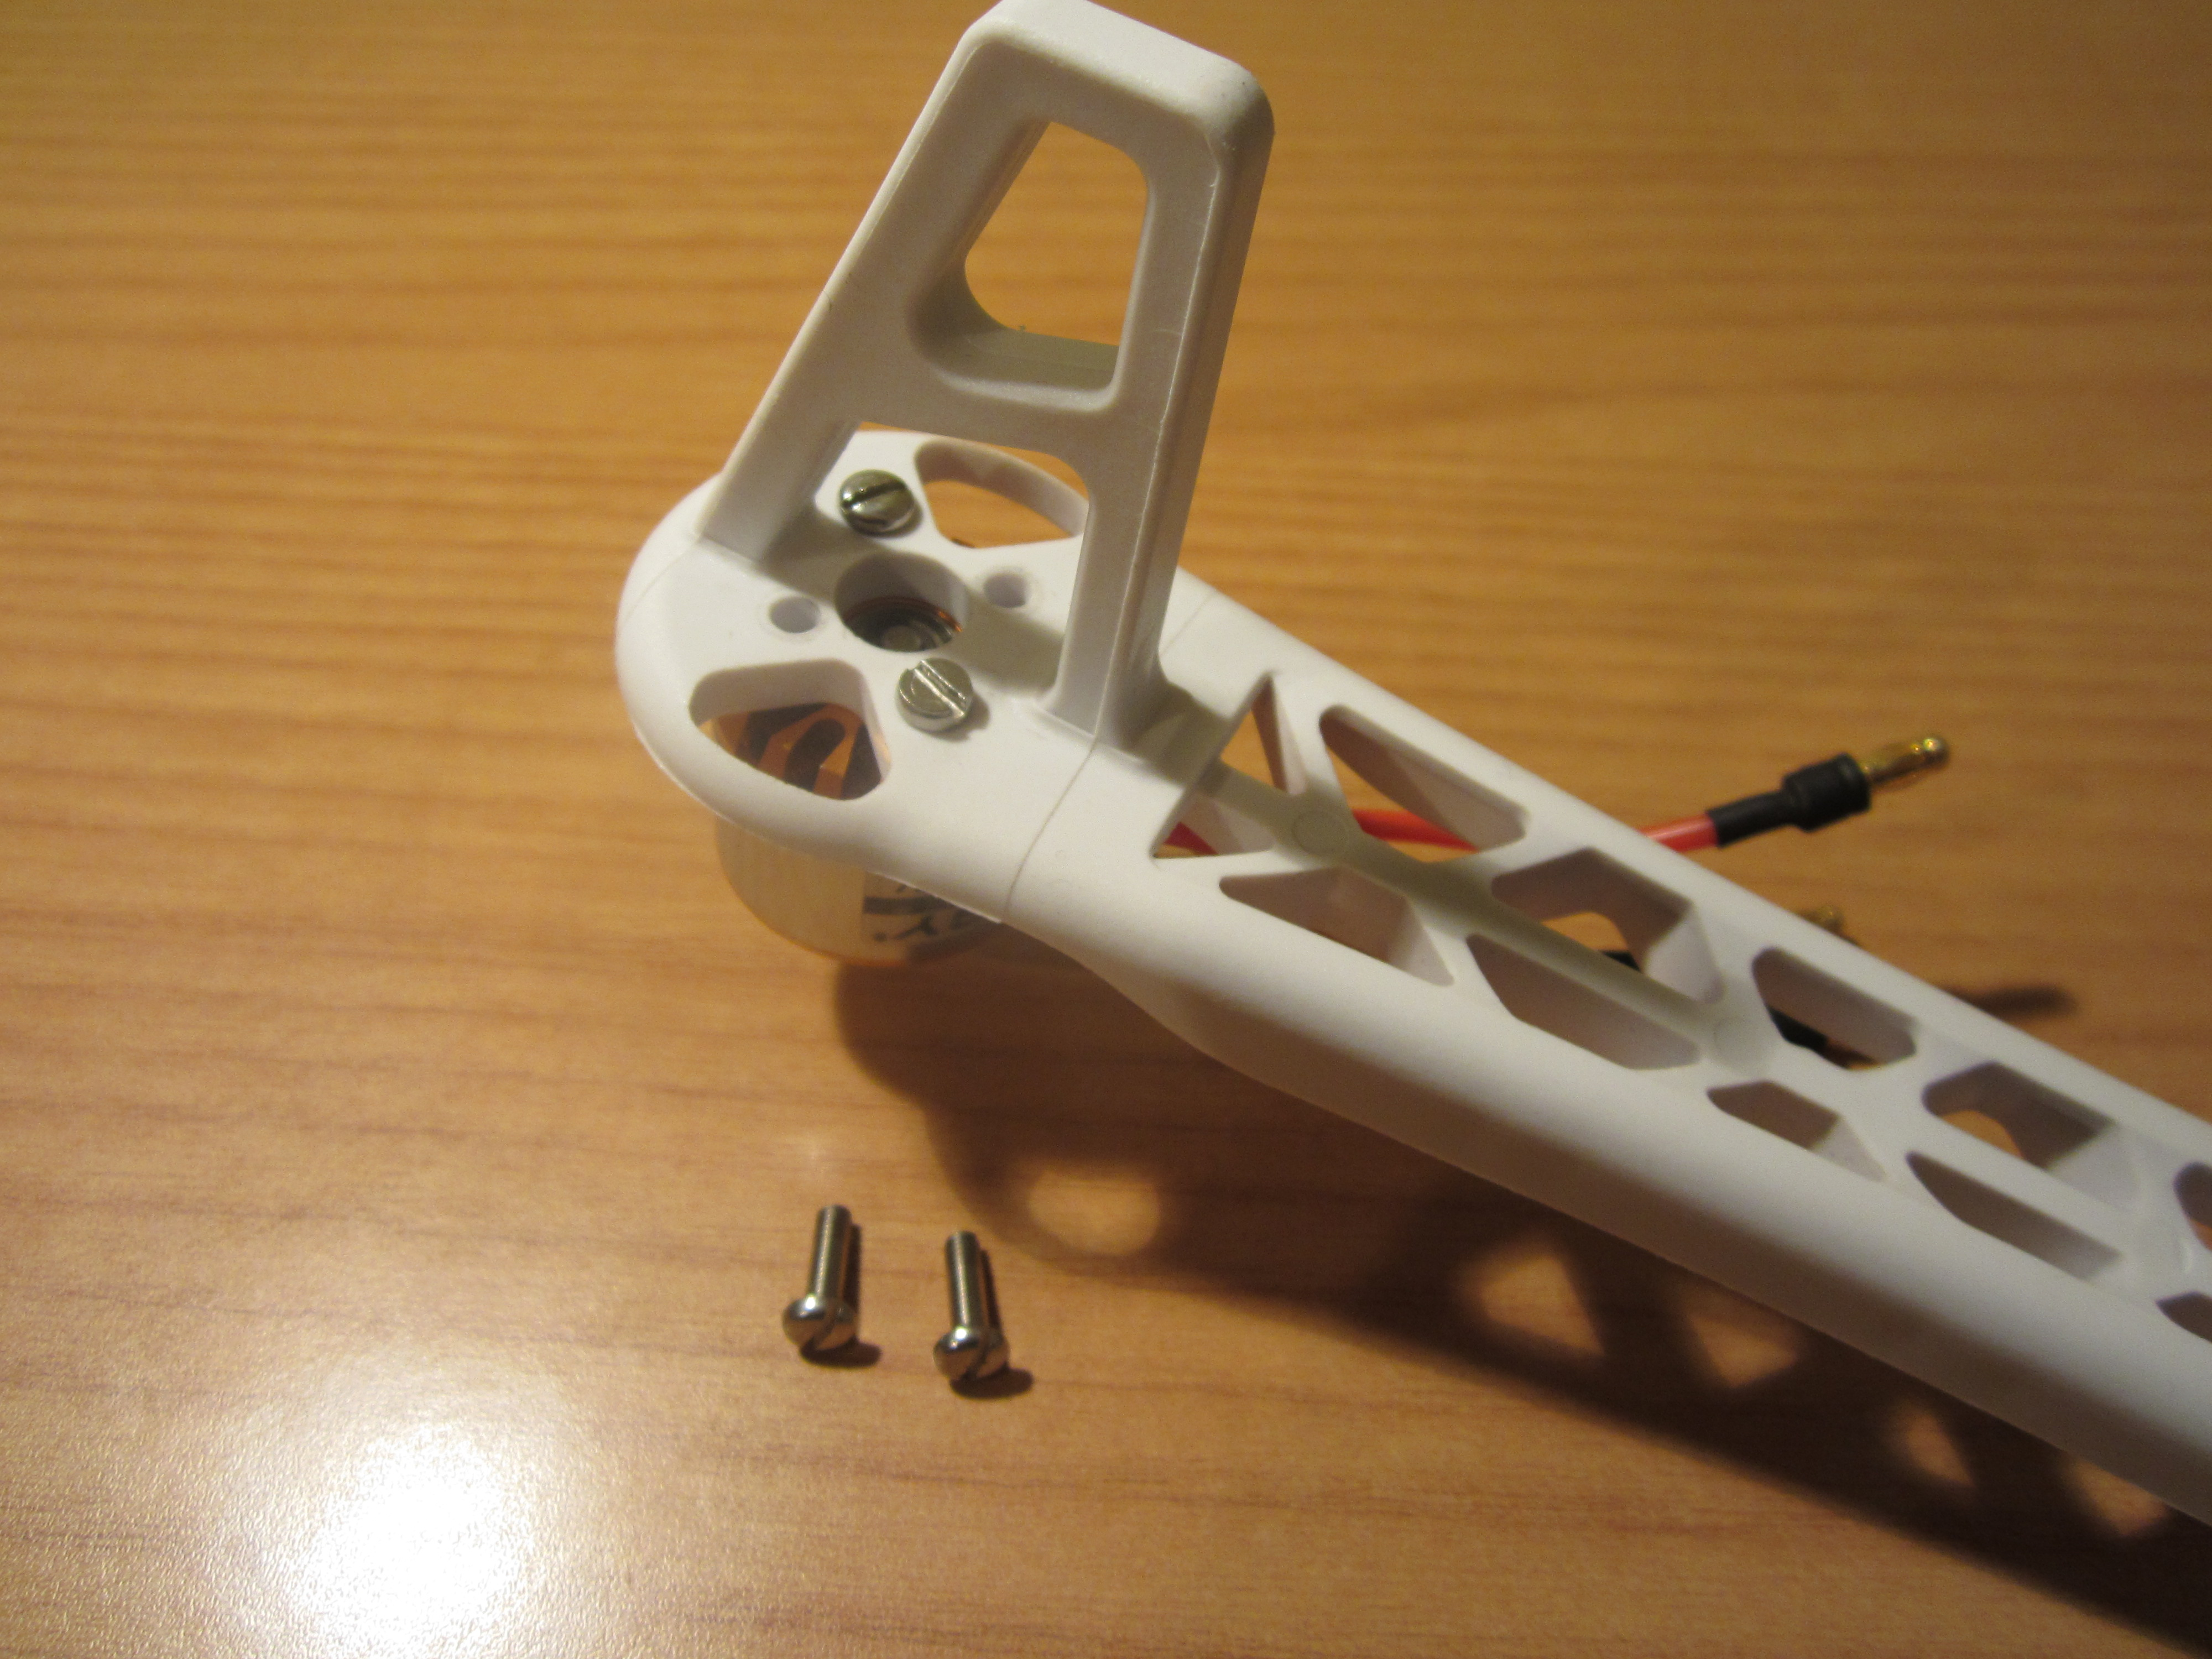
\includegraphics[width=0.8\linewidth]{Images/Mounting/IMG_0449.jpg}
  \captionof{figure}{}
  \label{diagScrews}
\end{minipage}%
\begin{minipage}{0.5\textwidth}
  \centering
  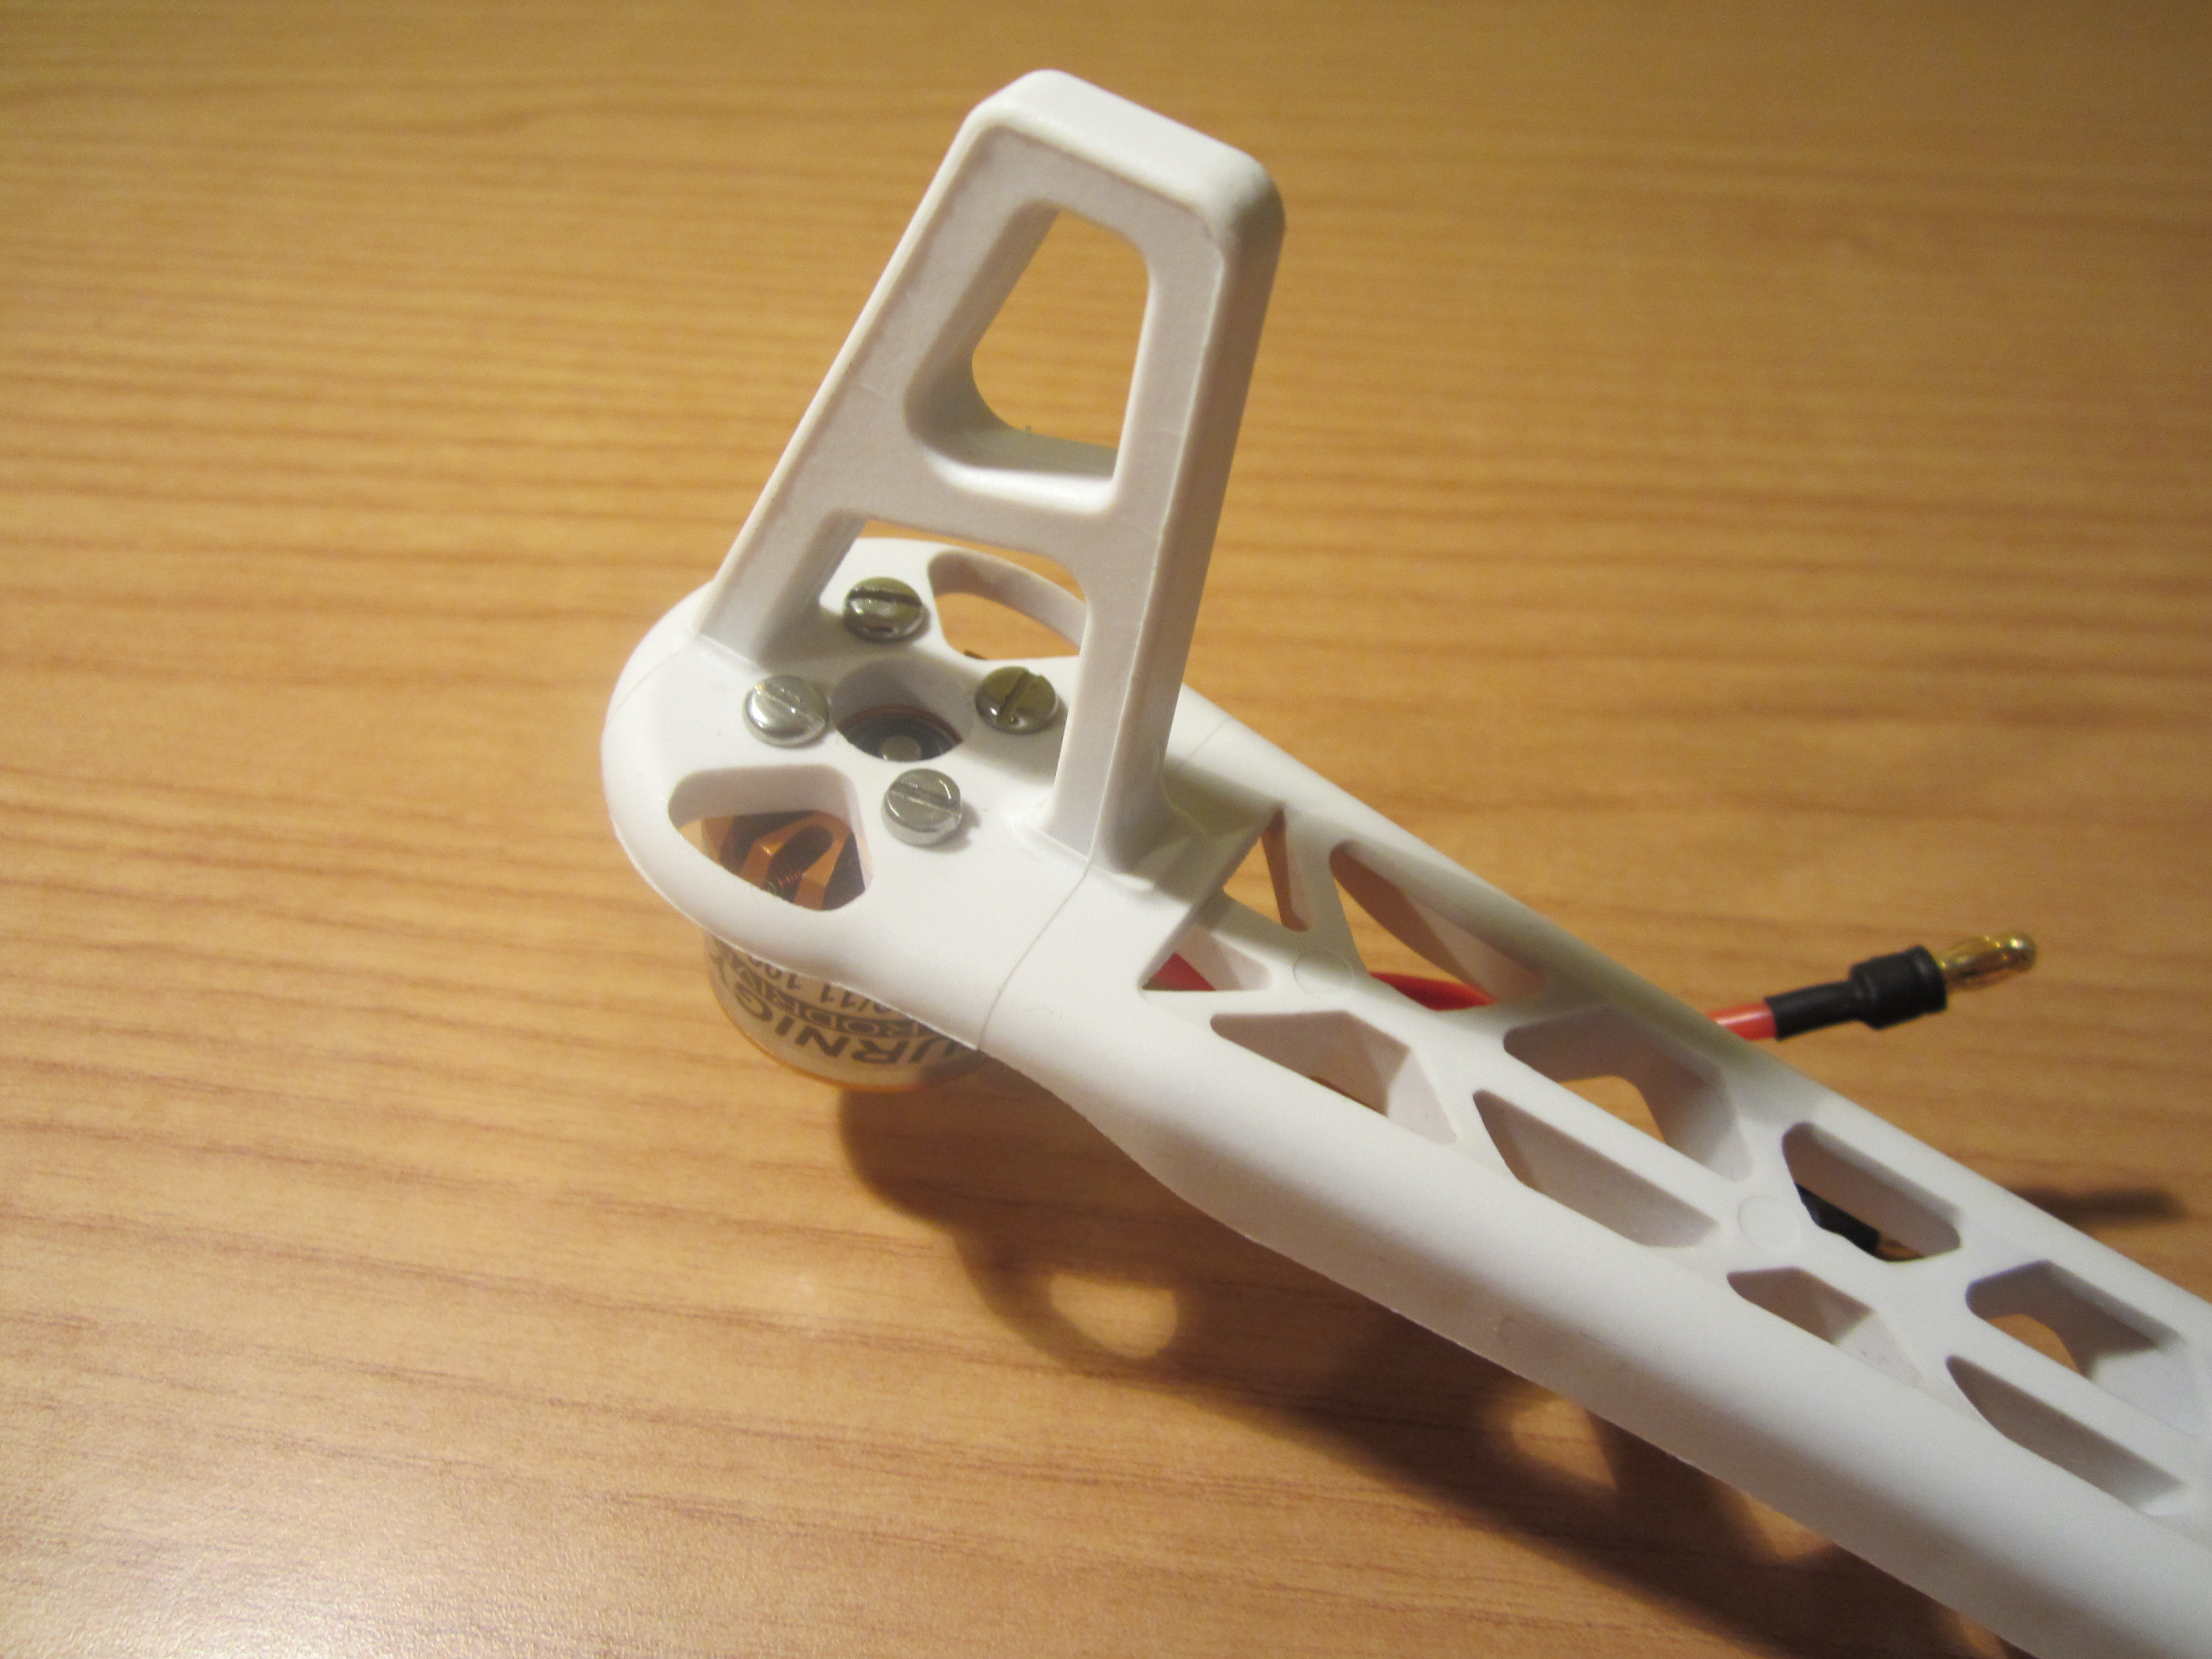
\includegraphics[width=0.8\linewidth]{Images/Mounting/IMG_0450.jpg}
  \captionof{figure}{}
  \label{allScrews}
\end{minipage}
\\[12pt]
\clearpage

If now we set the propeller on the motor we can see how they stand out a bit. This fact is not very important, however, it is recommended to trim the iron bar of about 0.5cm, so they are closer together.
\\[12pt]

\begin{minipage}{0.5\textwidth}
  \centering
  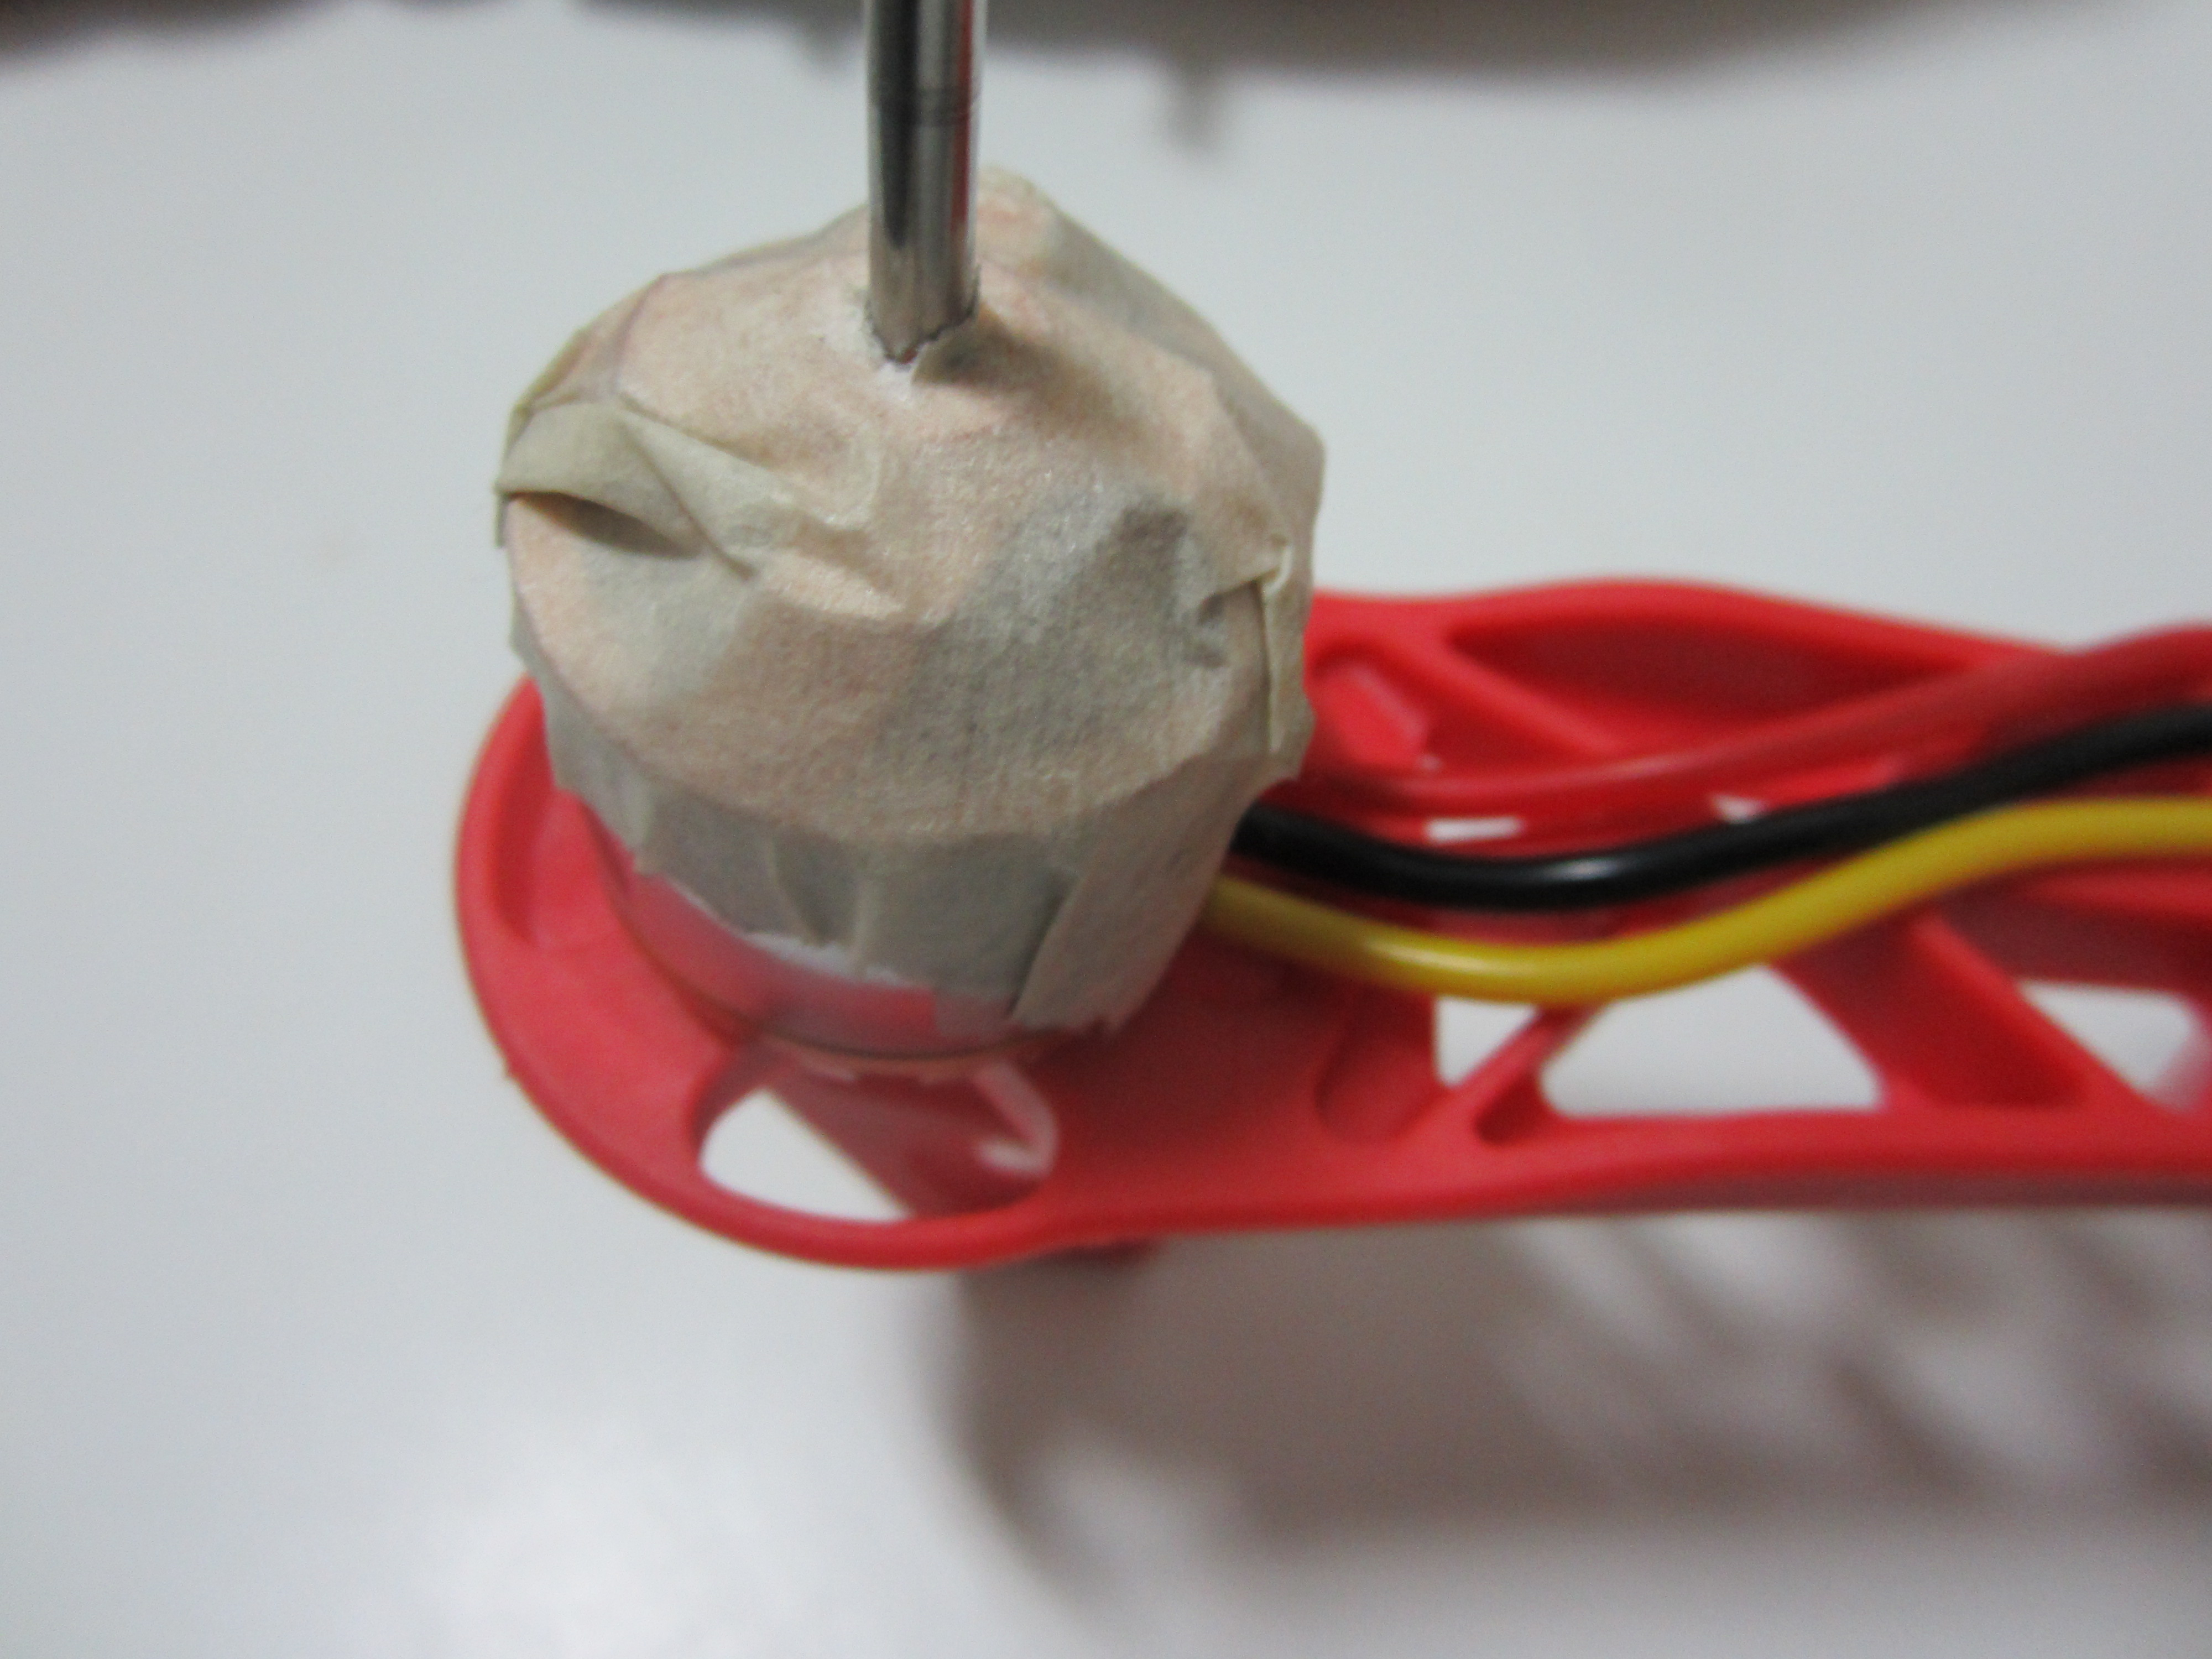
\includegraphics[width=0.8\linewidth]{Images/Mounting/IMG_0432.jpg}
  \captionof{figure}{}
  \label{fig:app1}
\end{minipage}%
\begin{minipage}{0.5\textwidth}
  \centering
  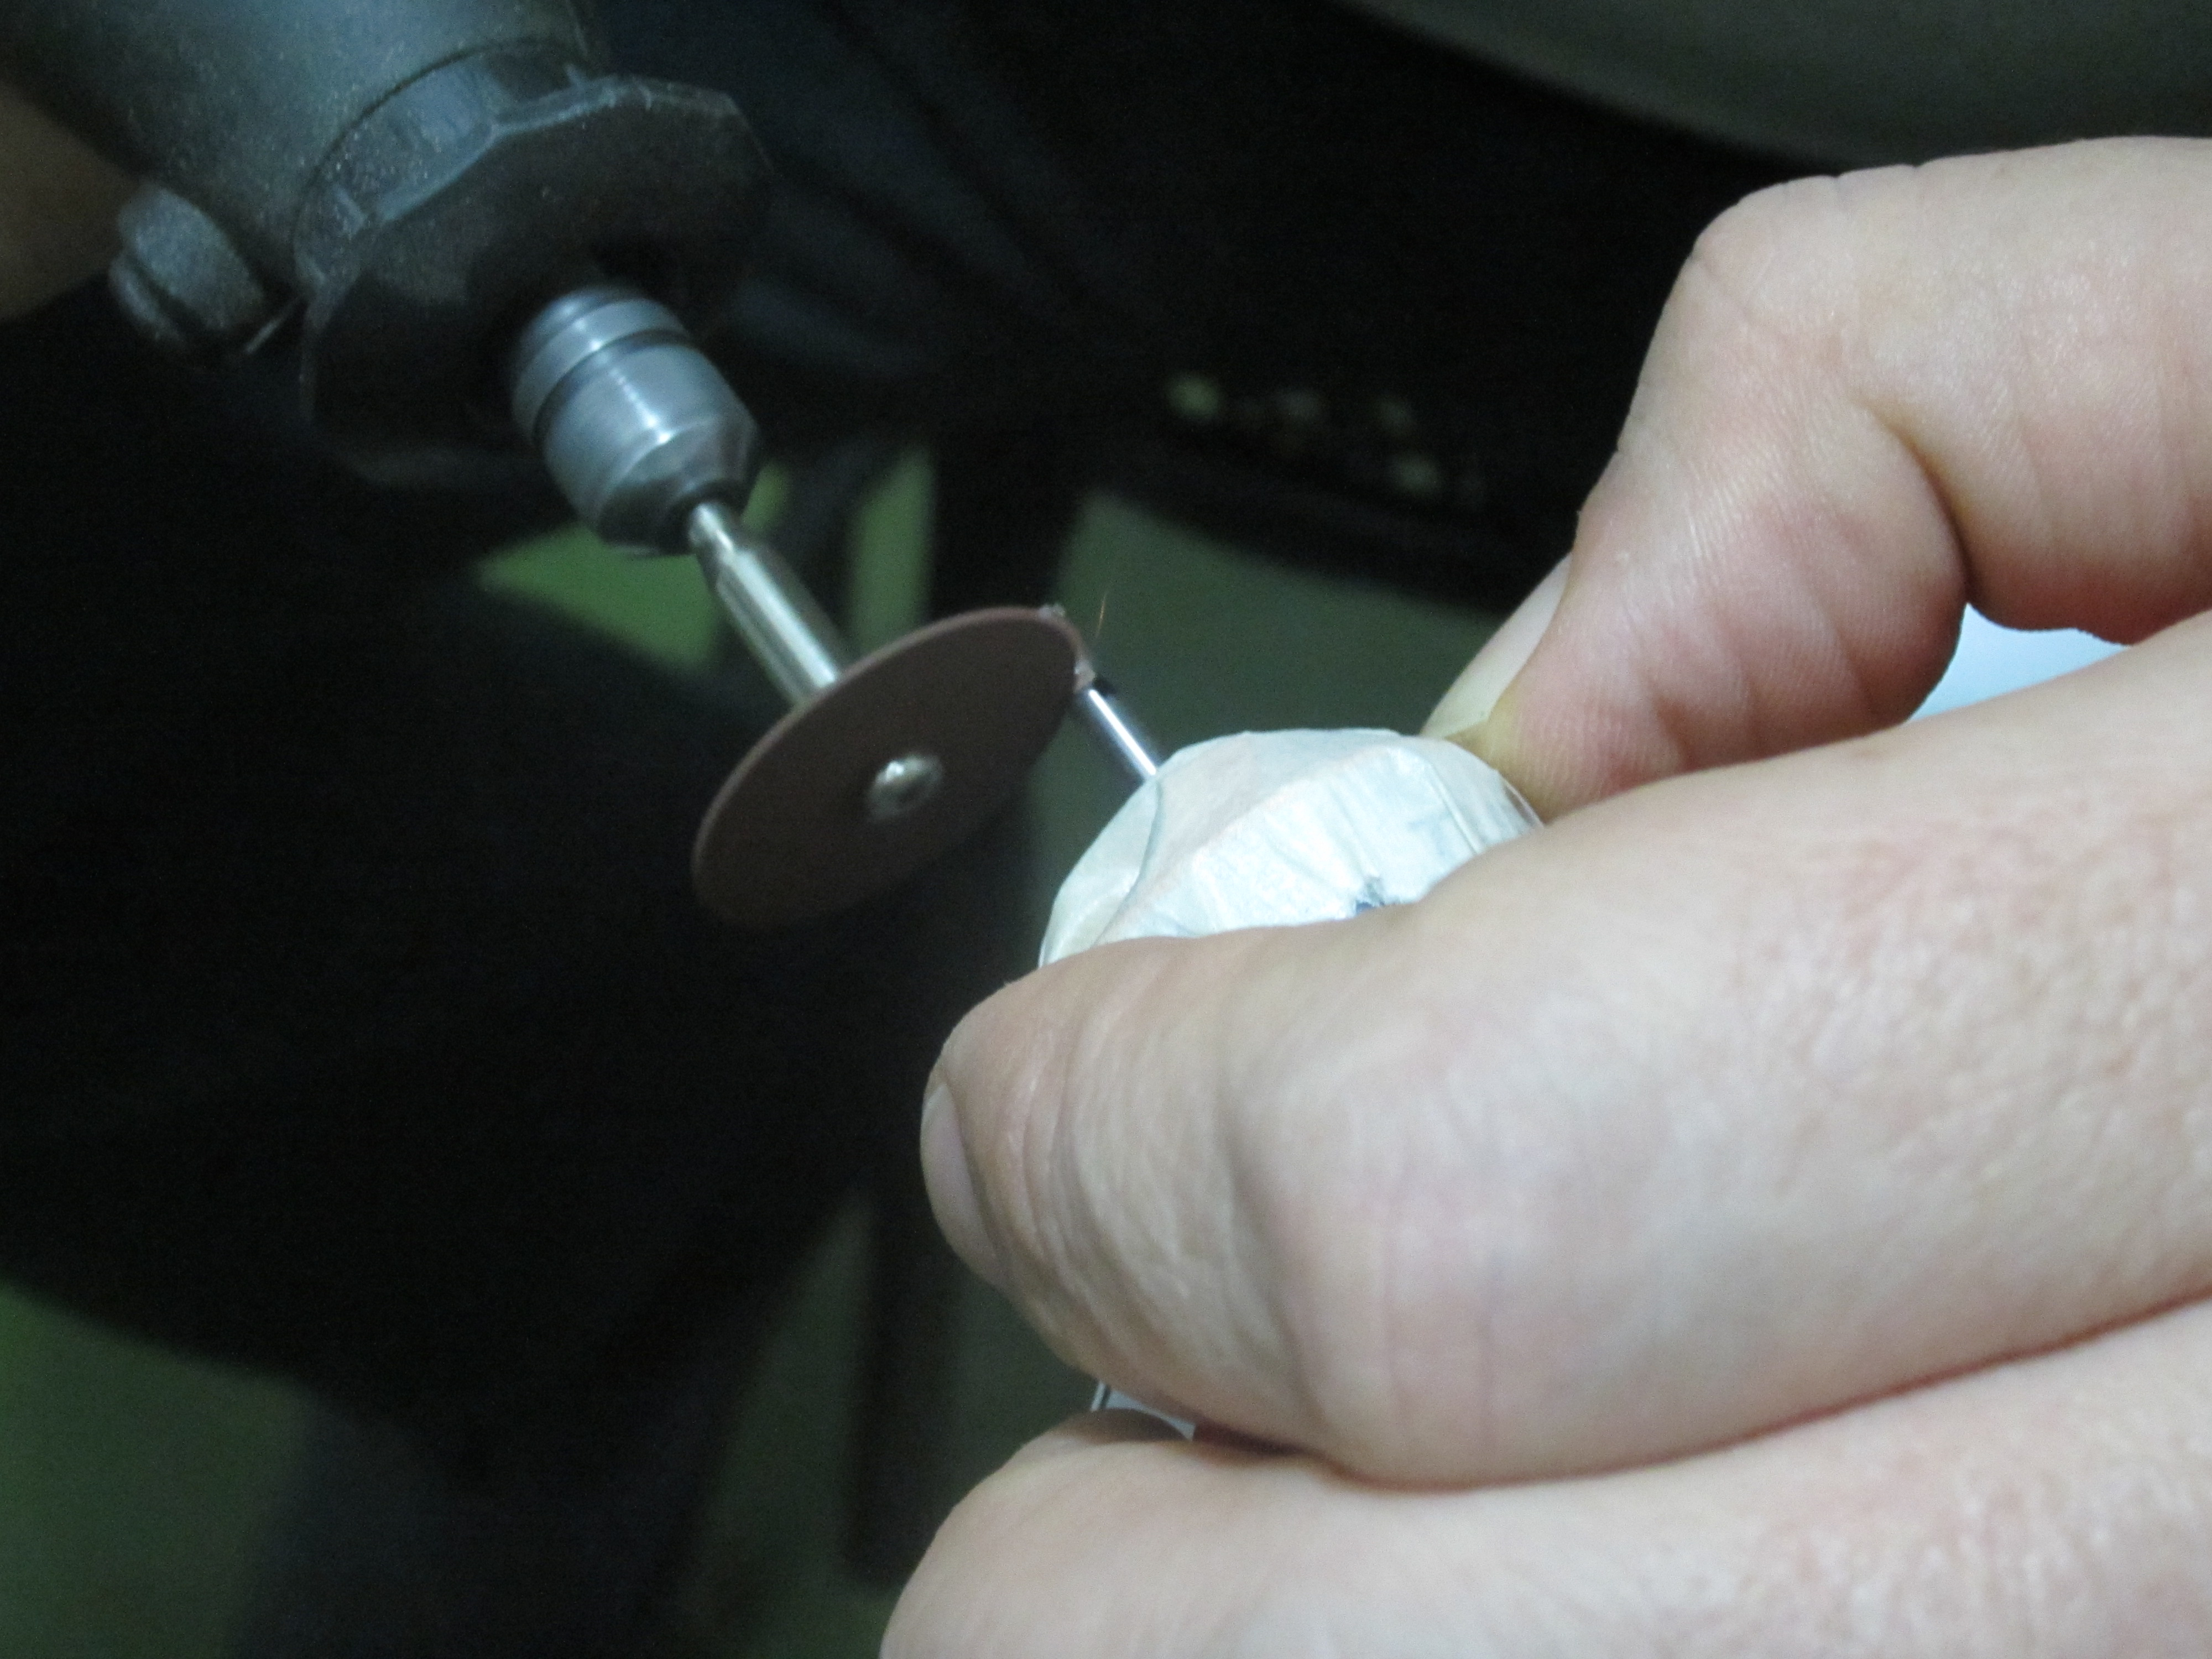
\includegraphics[width=0.8\linewidth]{Images/Mounting/IMG_0435.jpg}
  \captionof{figure}{}
  \label{fig:app2}
\end{minipage}

To perform this task we protect the engine from scrap when we cut, so it is recommended to drill a paper with iron or tape to cover the motor and prevent damage.

\noindent%
\begin{minipage}{\linewidth}
\vspace{10 mm}
\makebox[\linewidth]{%
  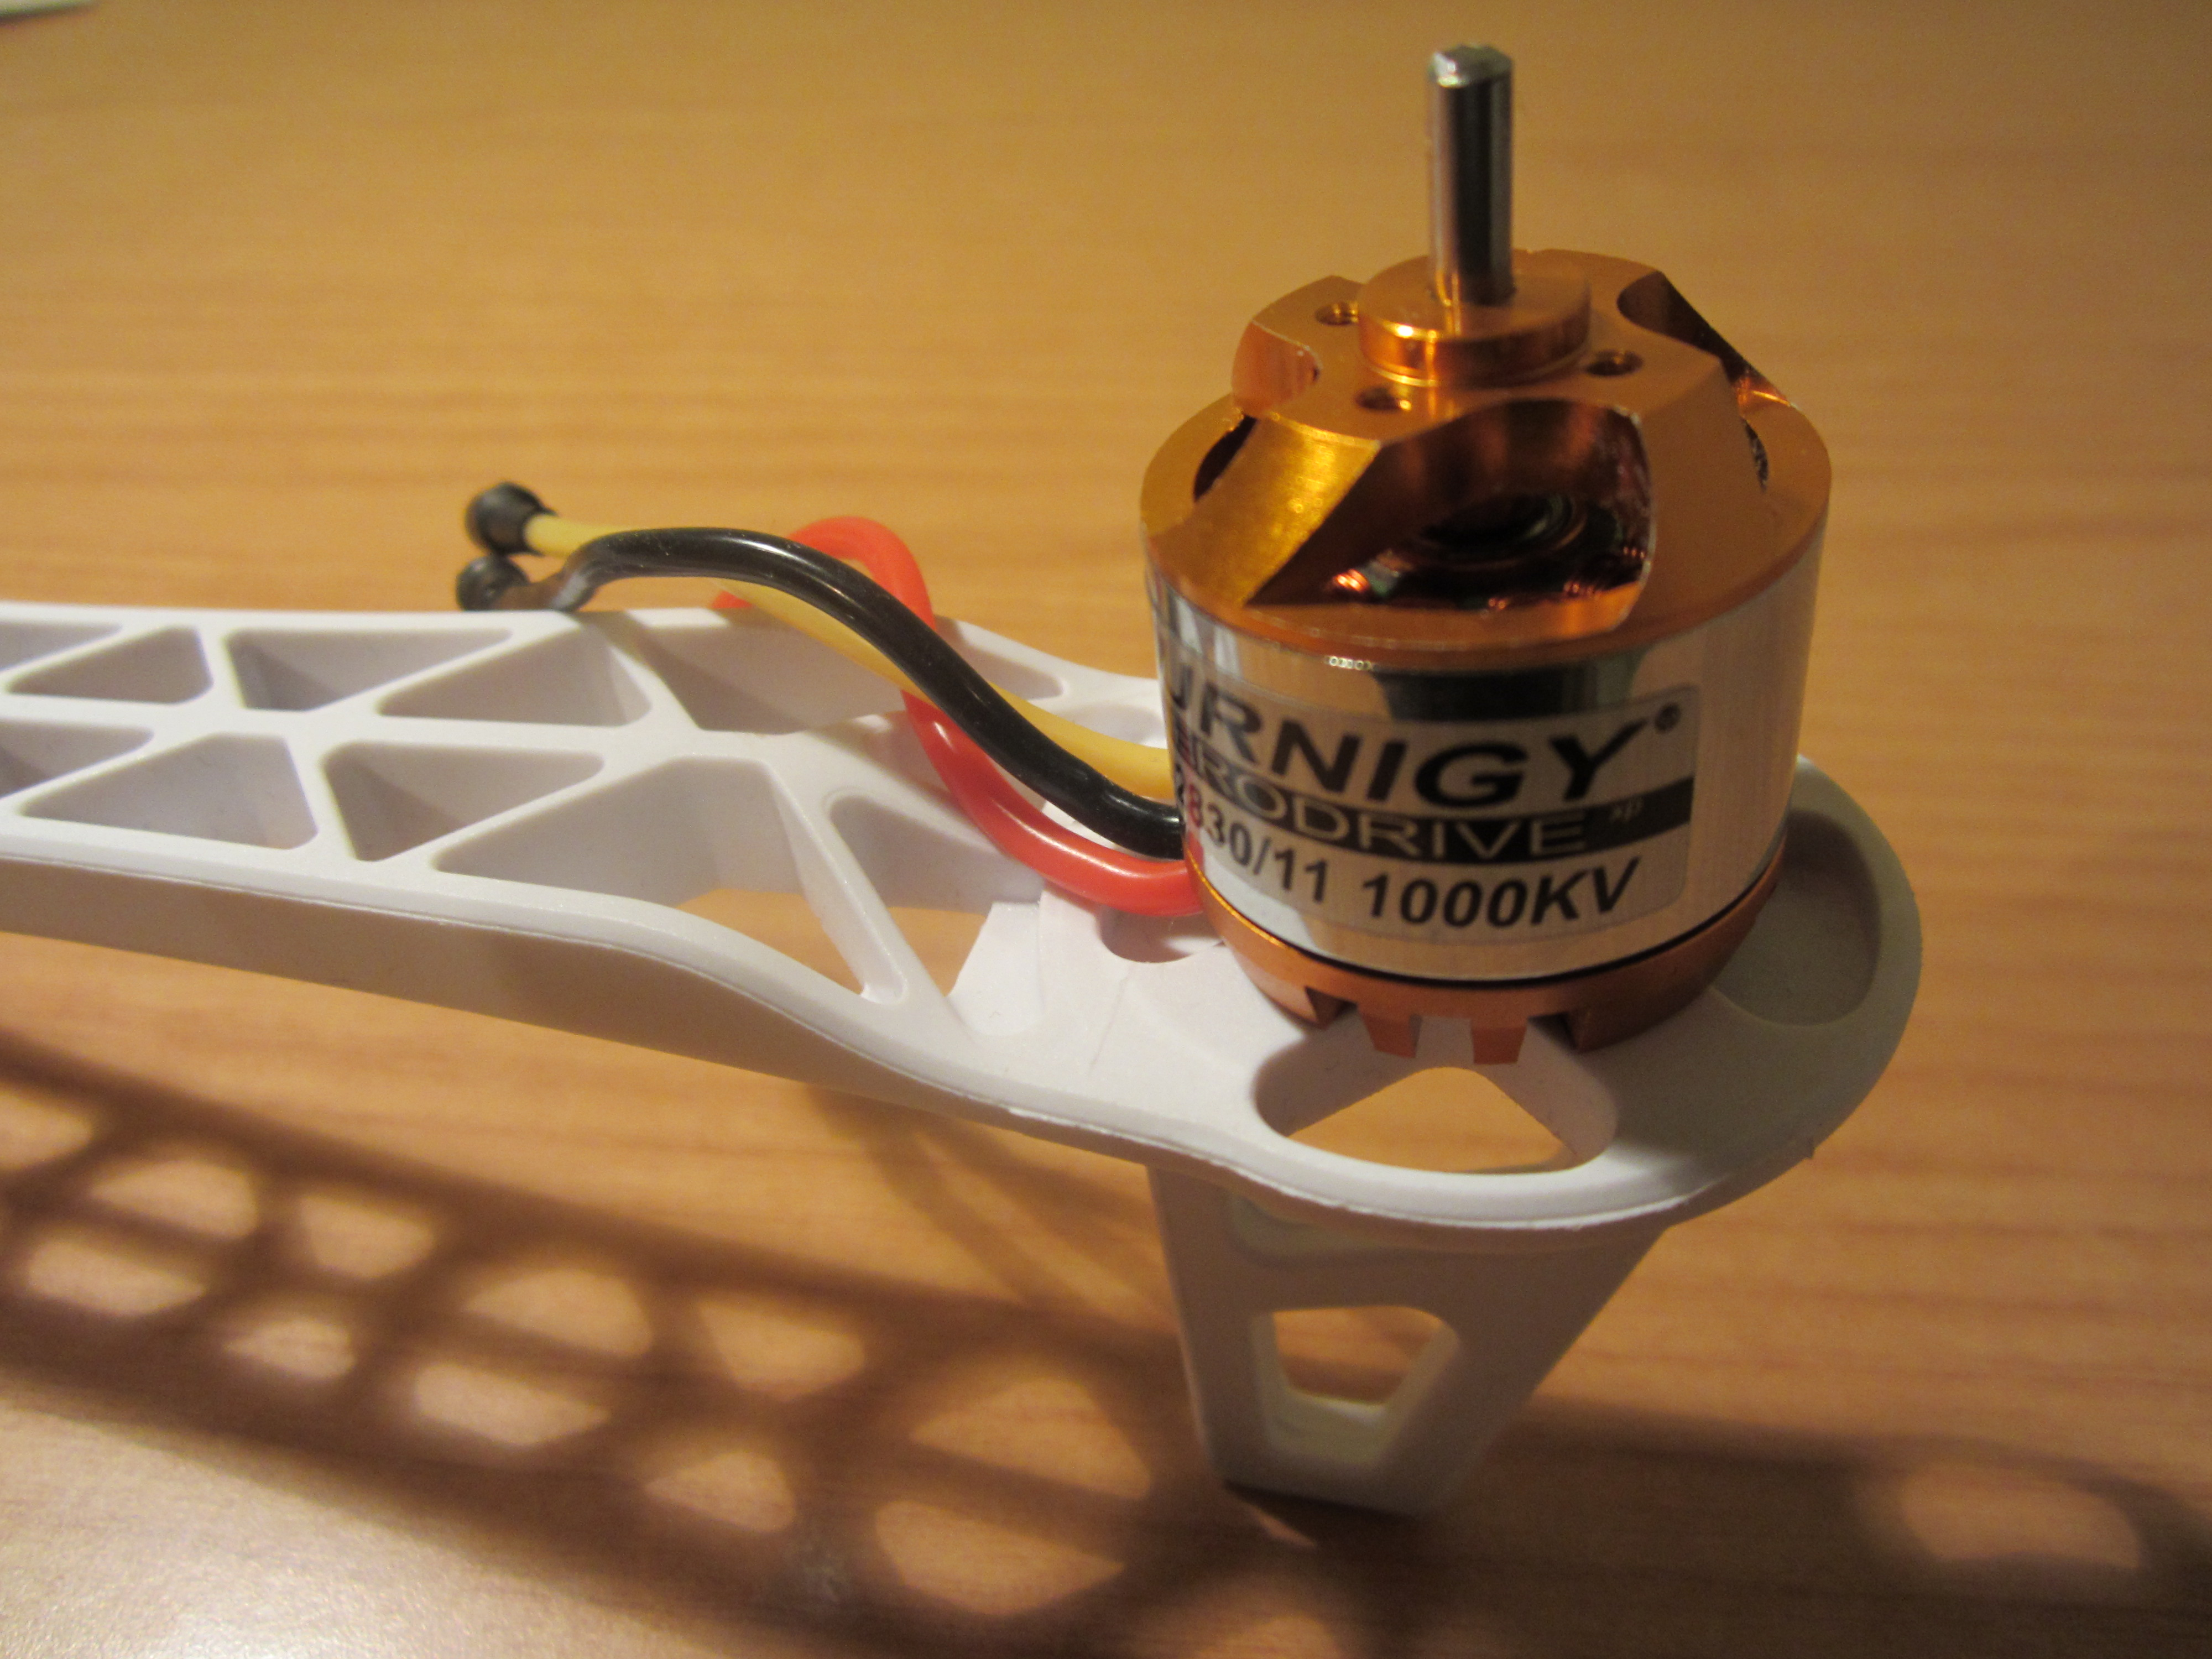
\includegraphics[width=0.8 \linewidth]{Images/Mounting/IMG_0452.jpg}}
\captionof{figure}{}% only if needed
\label{mobilenode1}
\end{minipage}    


\section{Base solders}

The wiring that connects the ESC to the base is too long, so it is recommended to cut the remaining wiring. This cut is approximately 1.5cm excluding the connector. After that, do not forget about to peel 0.5cm of cable in order to solder it correctly.
\\[12 pt]

\begin{minipage}{0.5\textwidth}
  \centering
  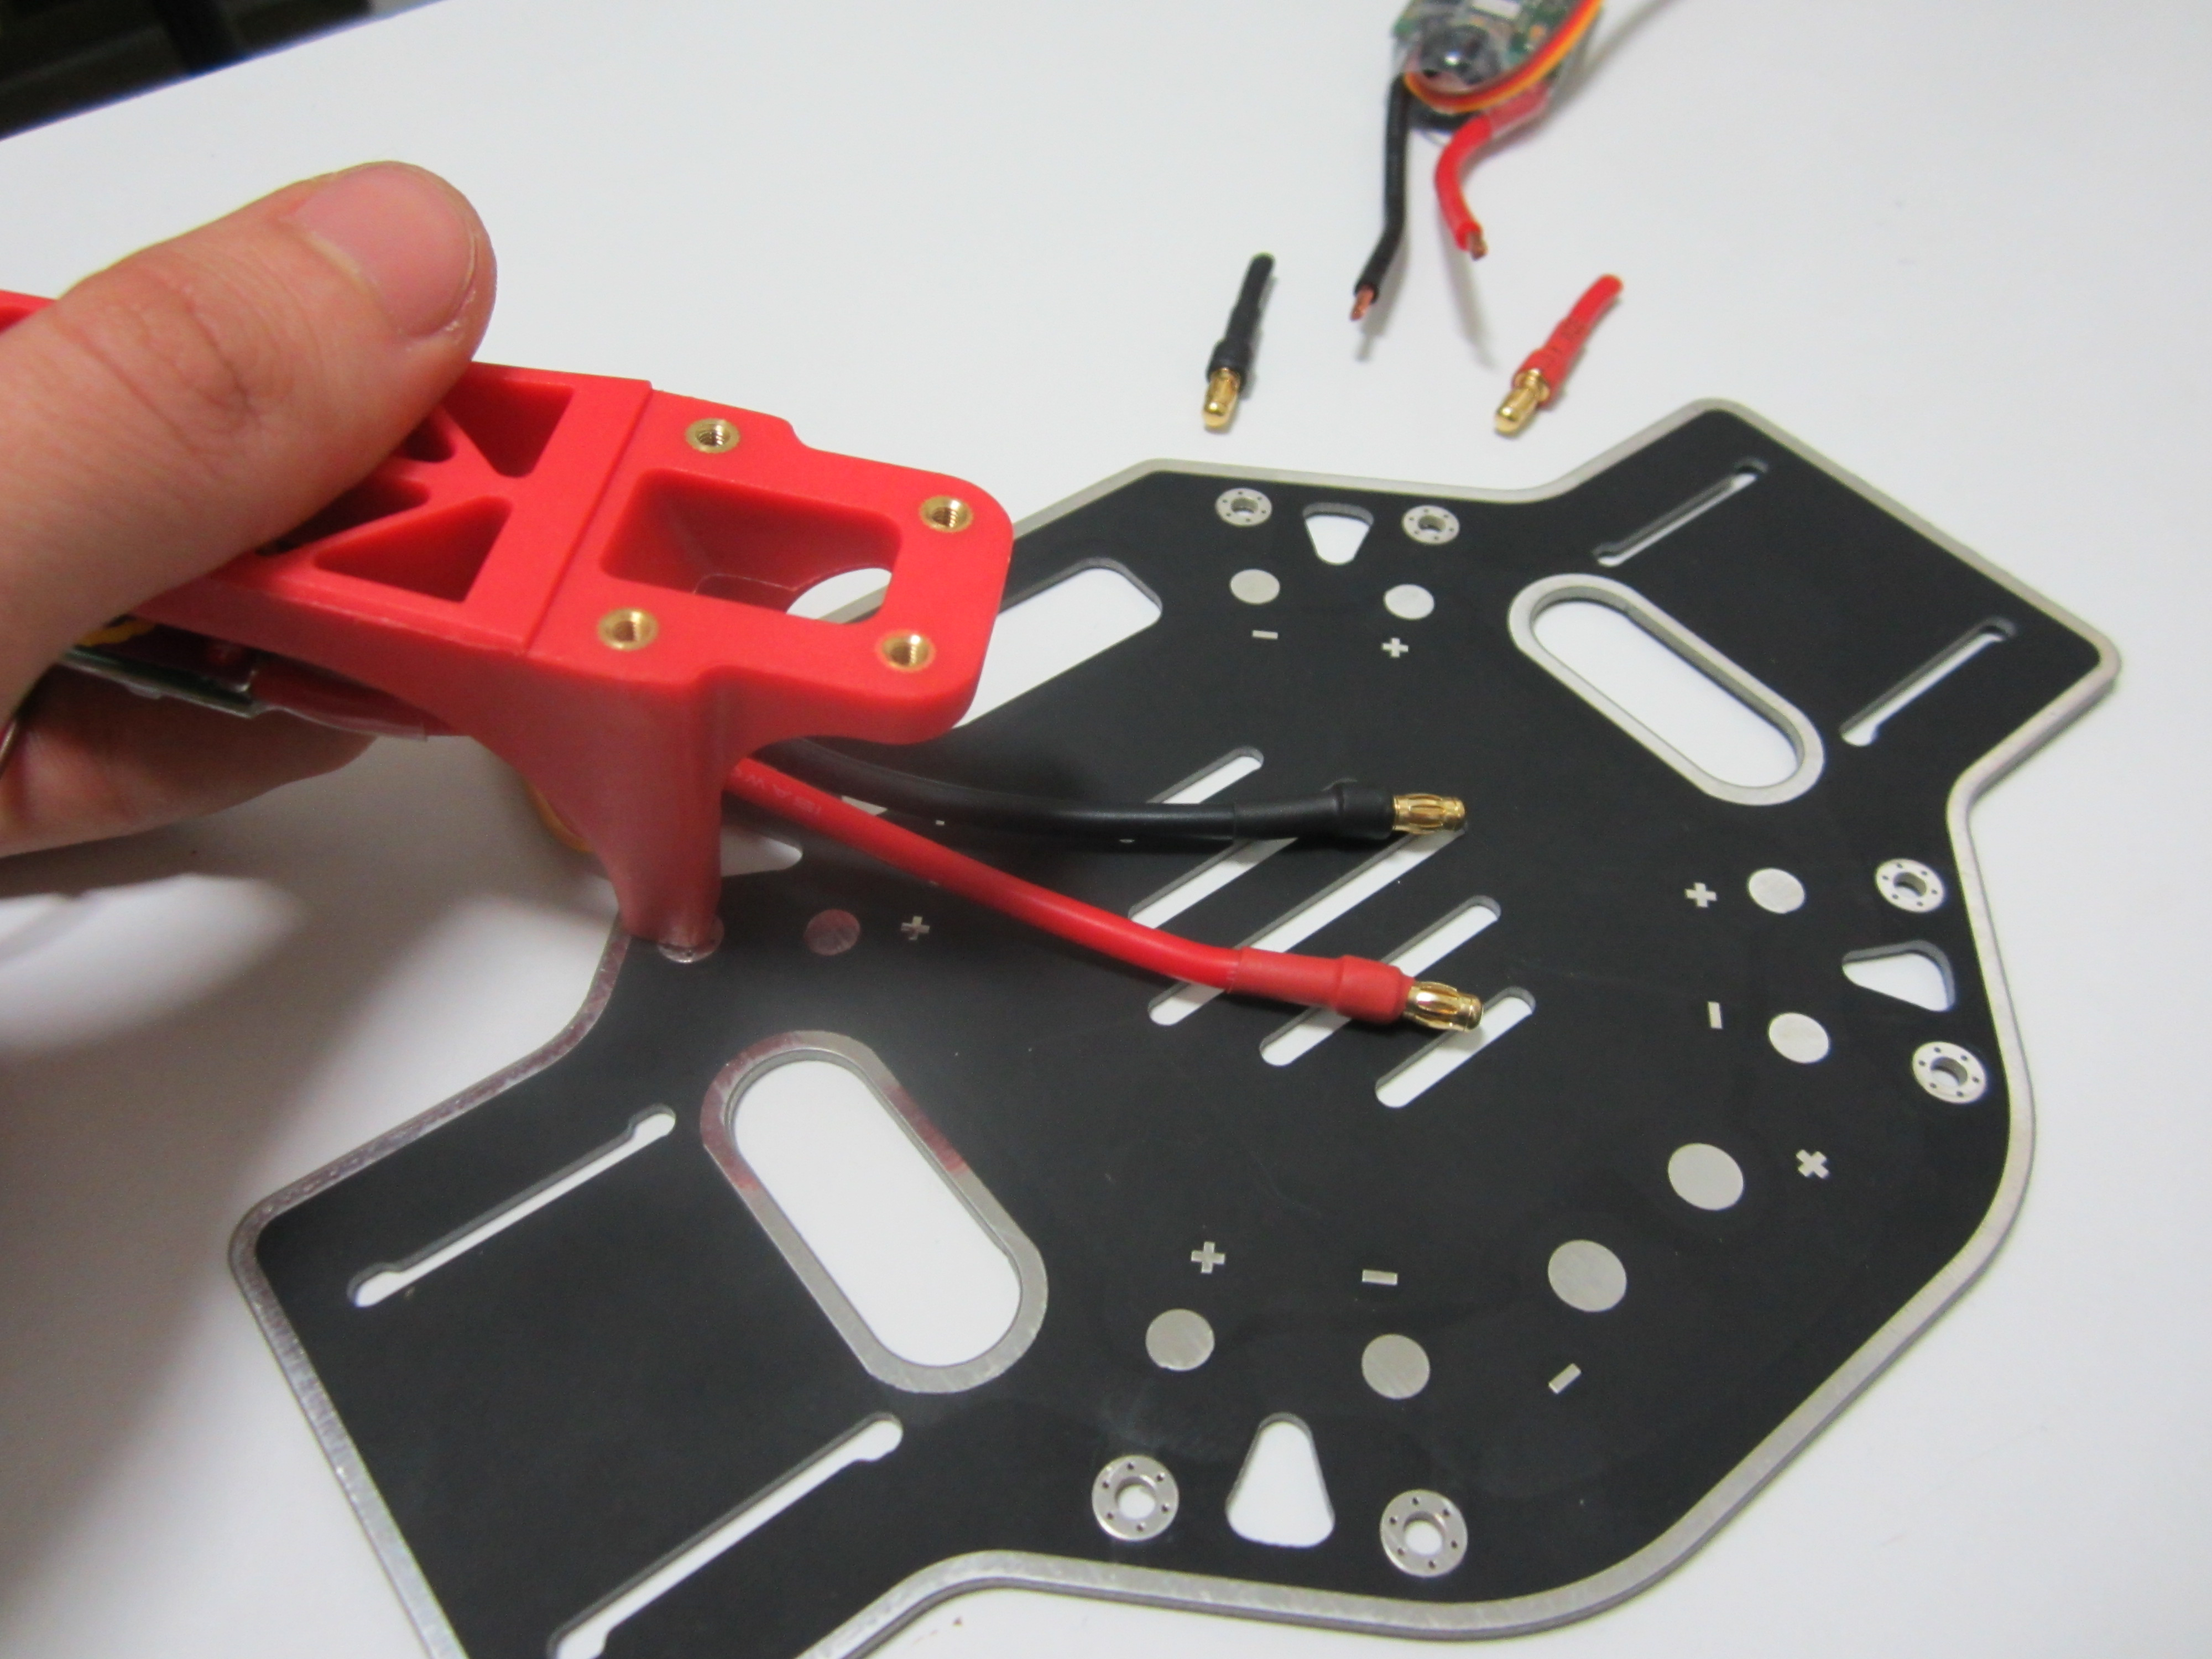
\includegraphics[width=0.8\linewidth]{Images/Mounting/IMG_0366.jpg}
  \captionof{figure}{}
  \label{fig:app1}
\end{minipage}%
\begin{minipage}{0.5\textwidth}
  \centering
  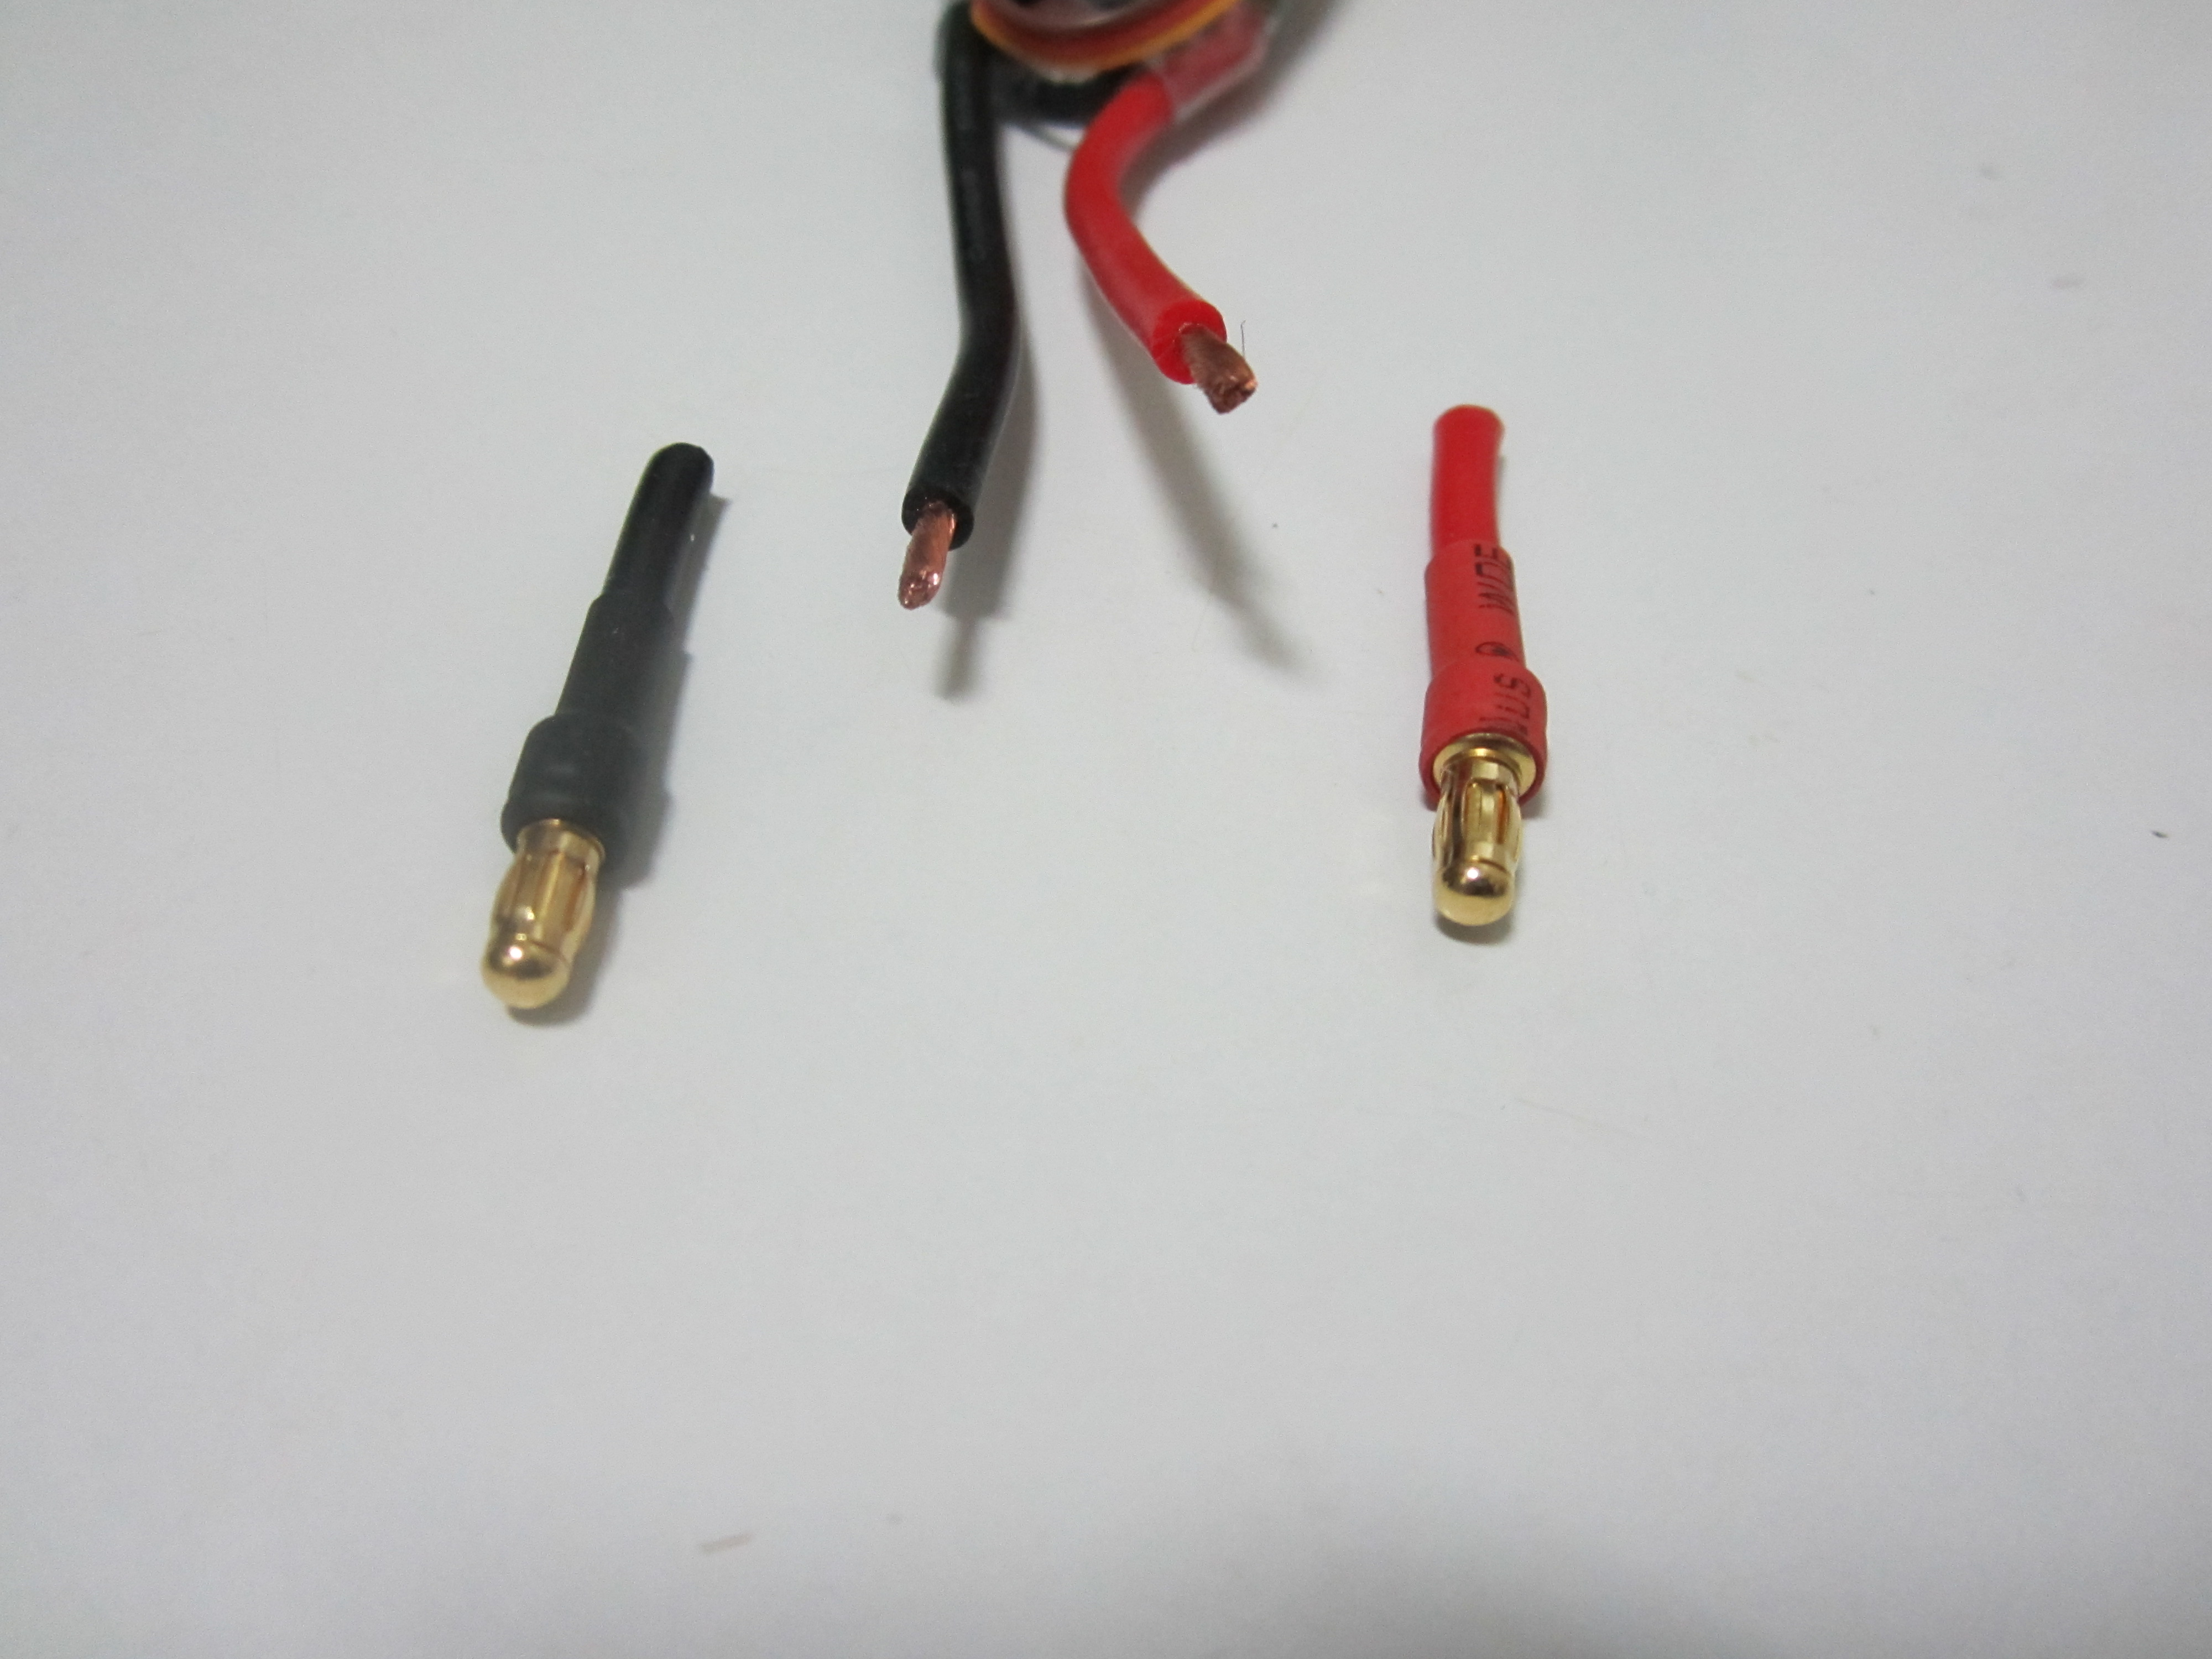
\includegraphics[width=0.8\linewidth]{Images/Mounting/IMG_0368.jpg}
  \captionof{figure}{}
  \label{fig:app2}
\end{minipage}


Soldering process
\\[12 pt]

\begin{minipage}{0.5\textwidth}
  \centering
  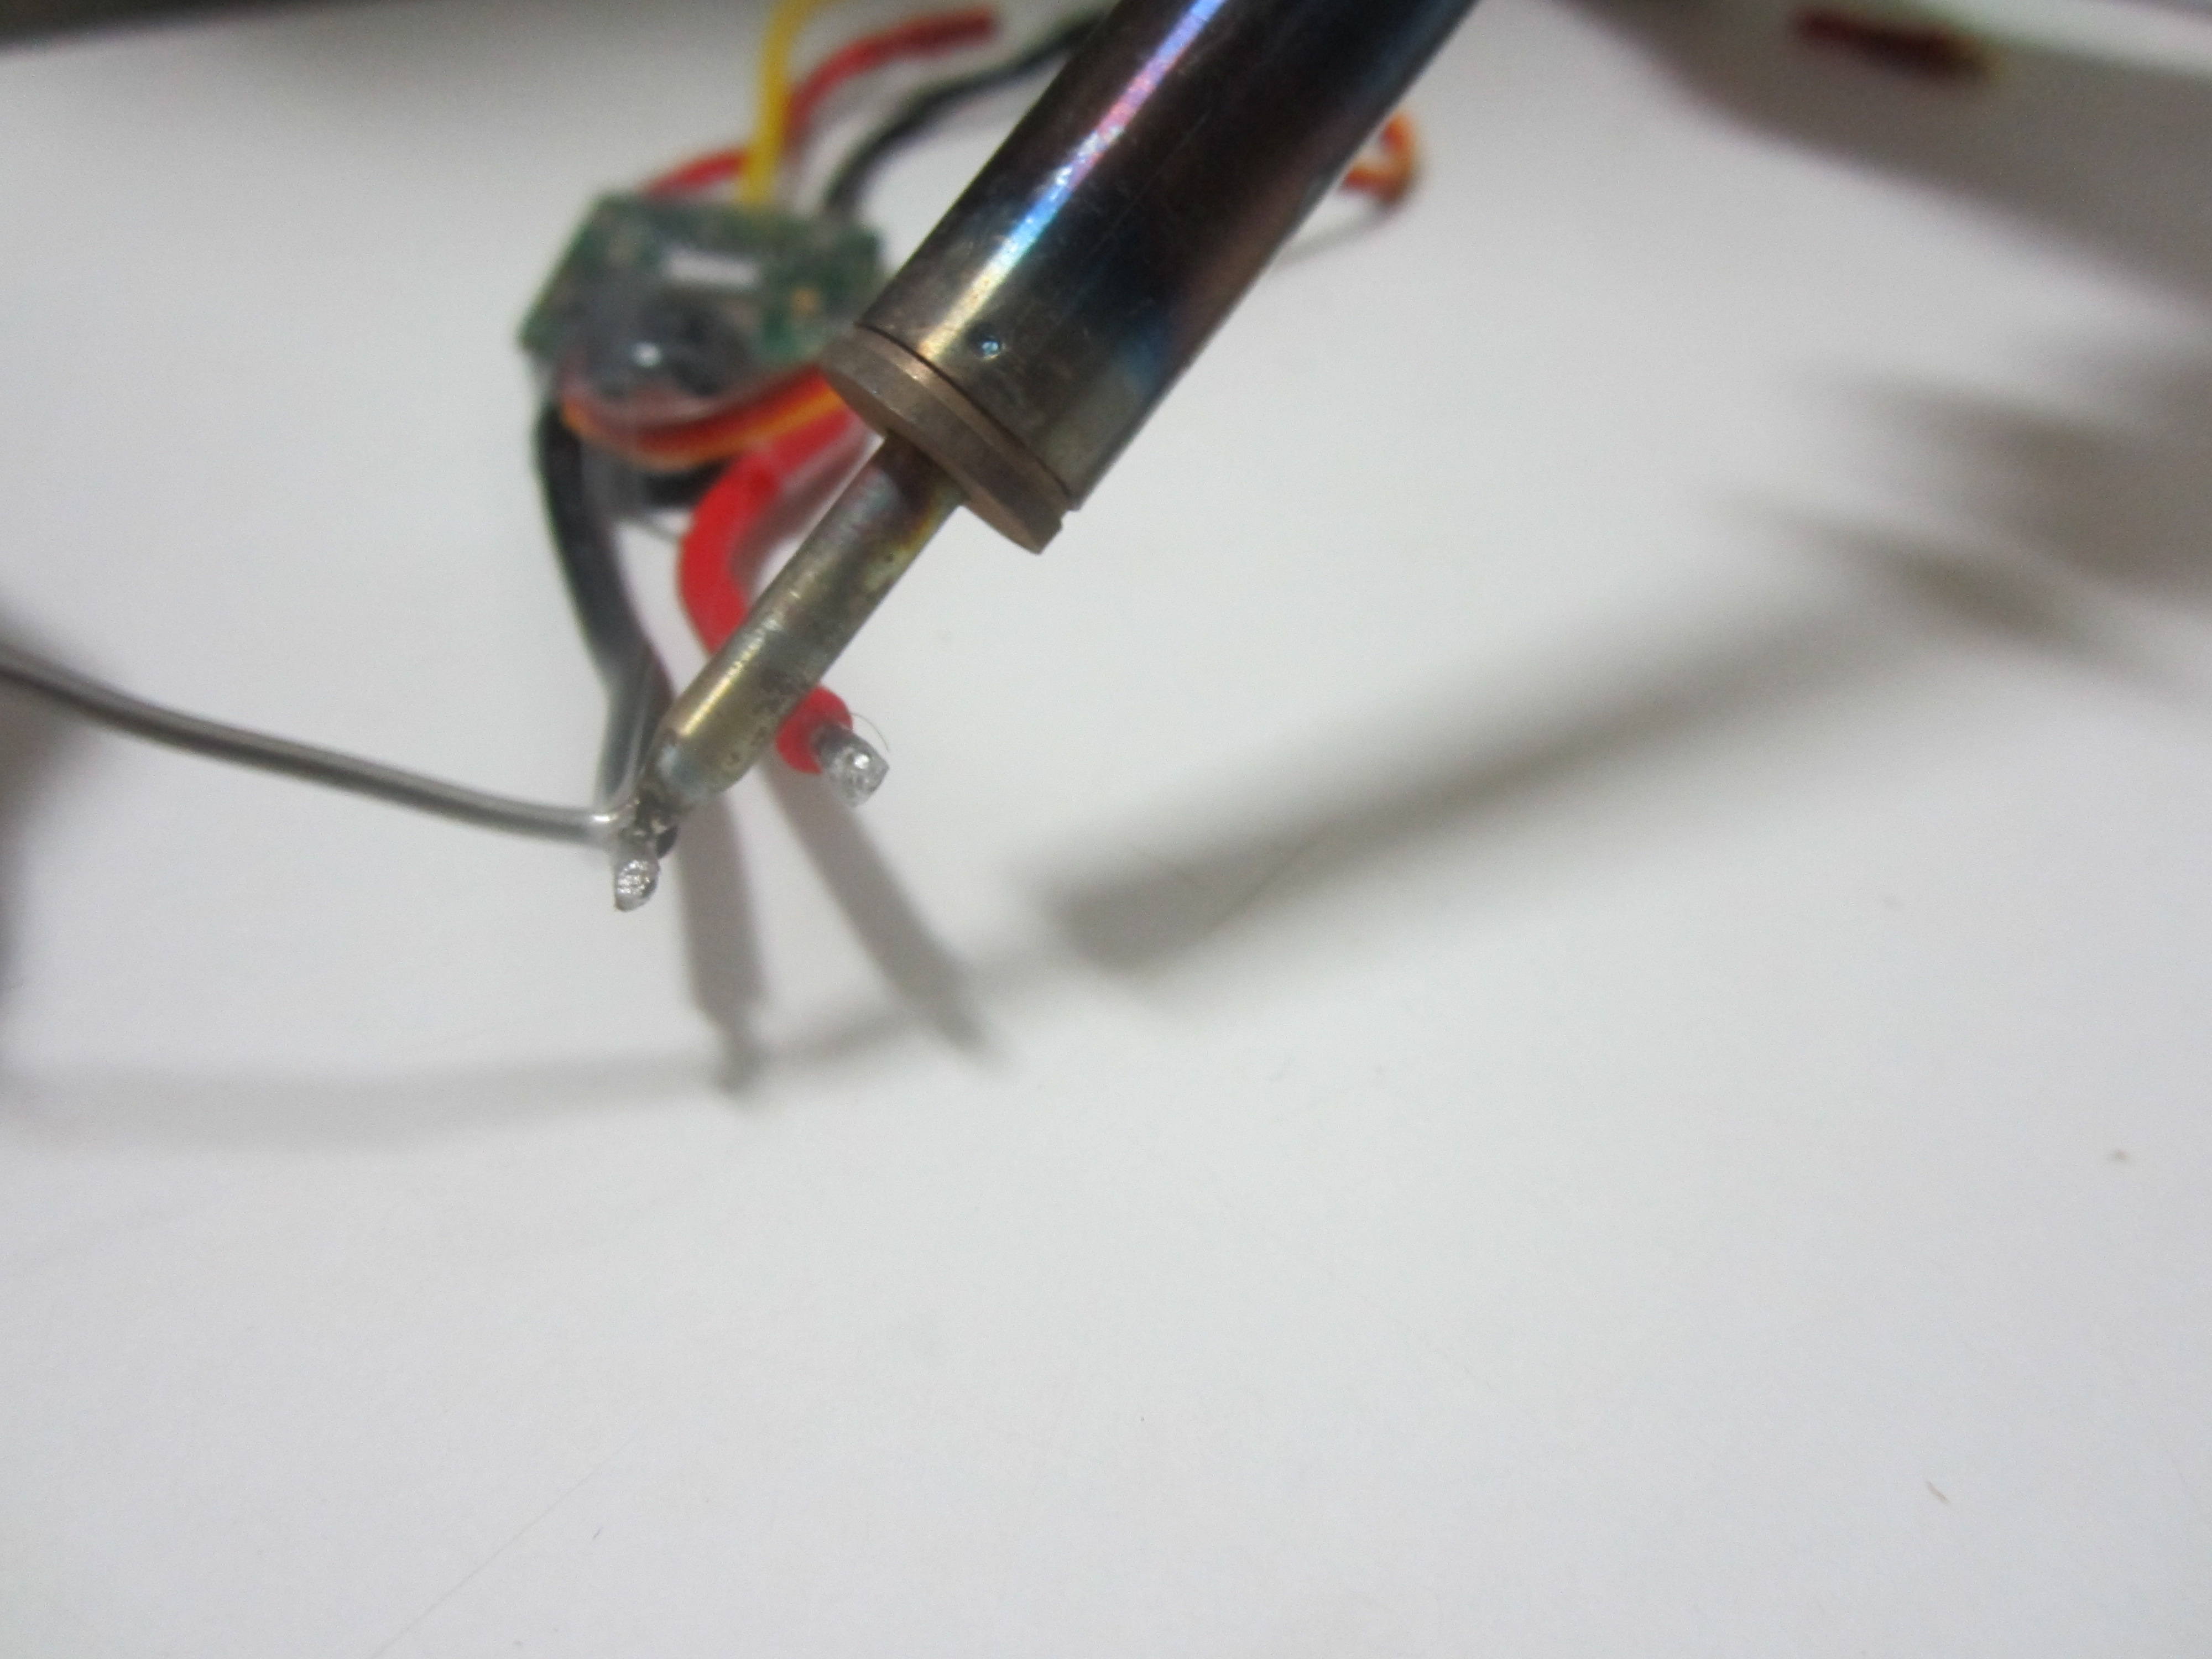
\includegraphics[width=0.8\linewidth]{Images/Mounting/IMG_0371.jpg}
  \captionof{figure}{}
  \label{fig:app1}
\end{minipage}%
\begin{minipage}{0.5\textwidth}
  \centering
  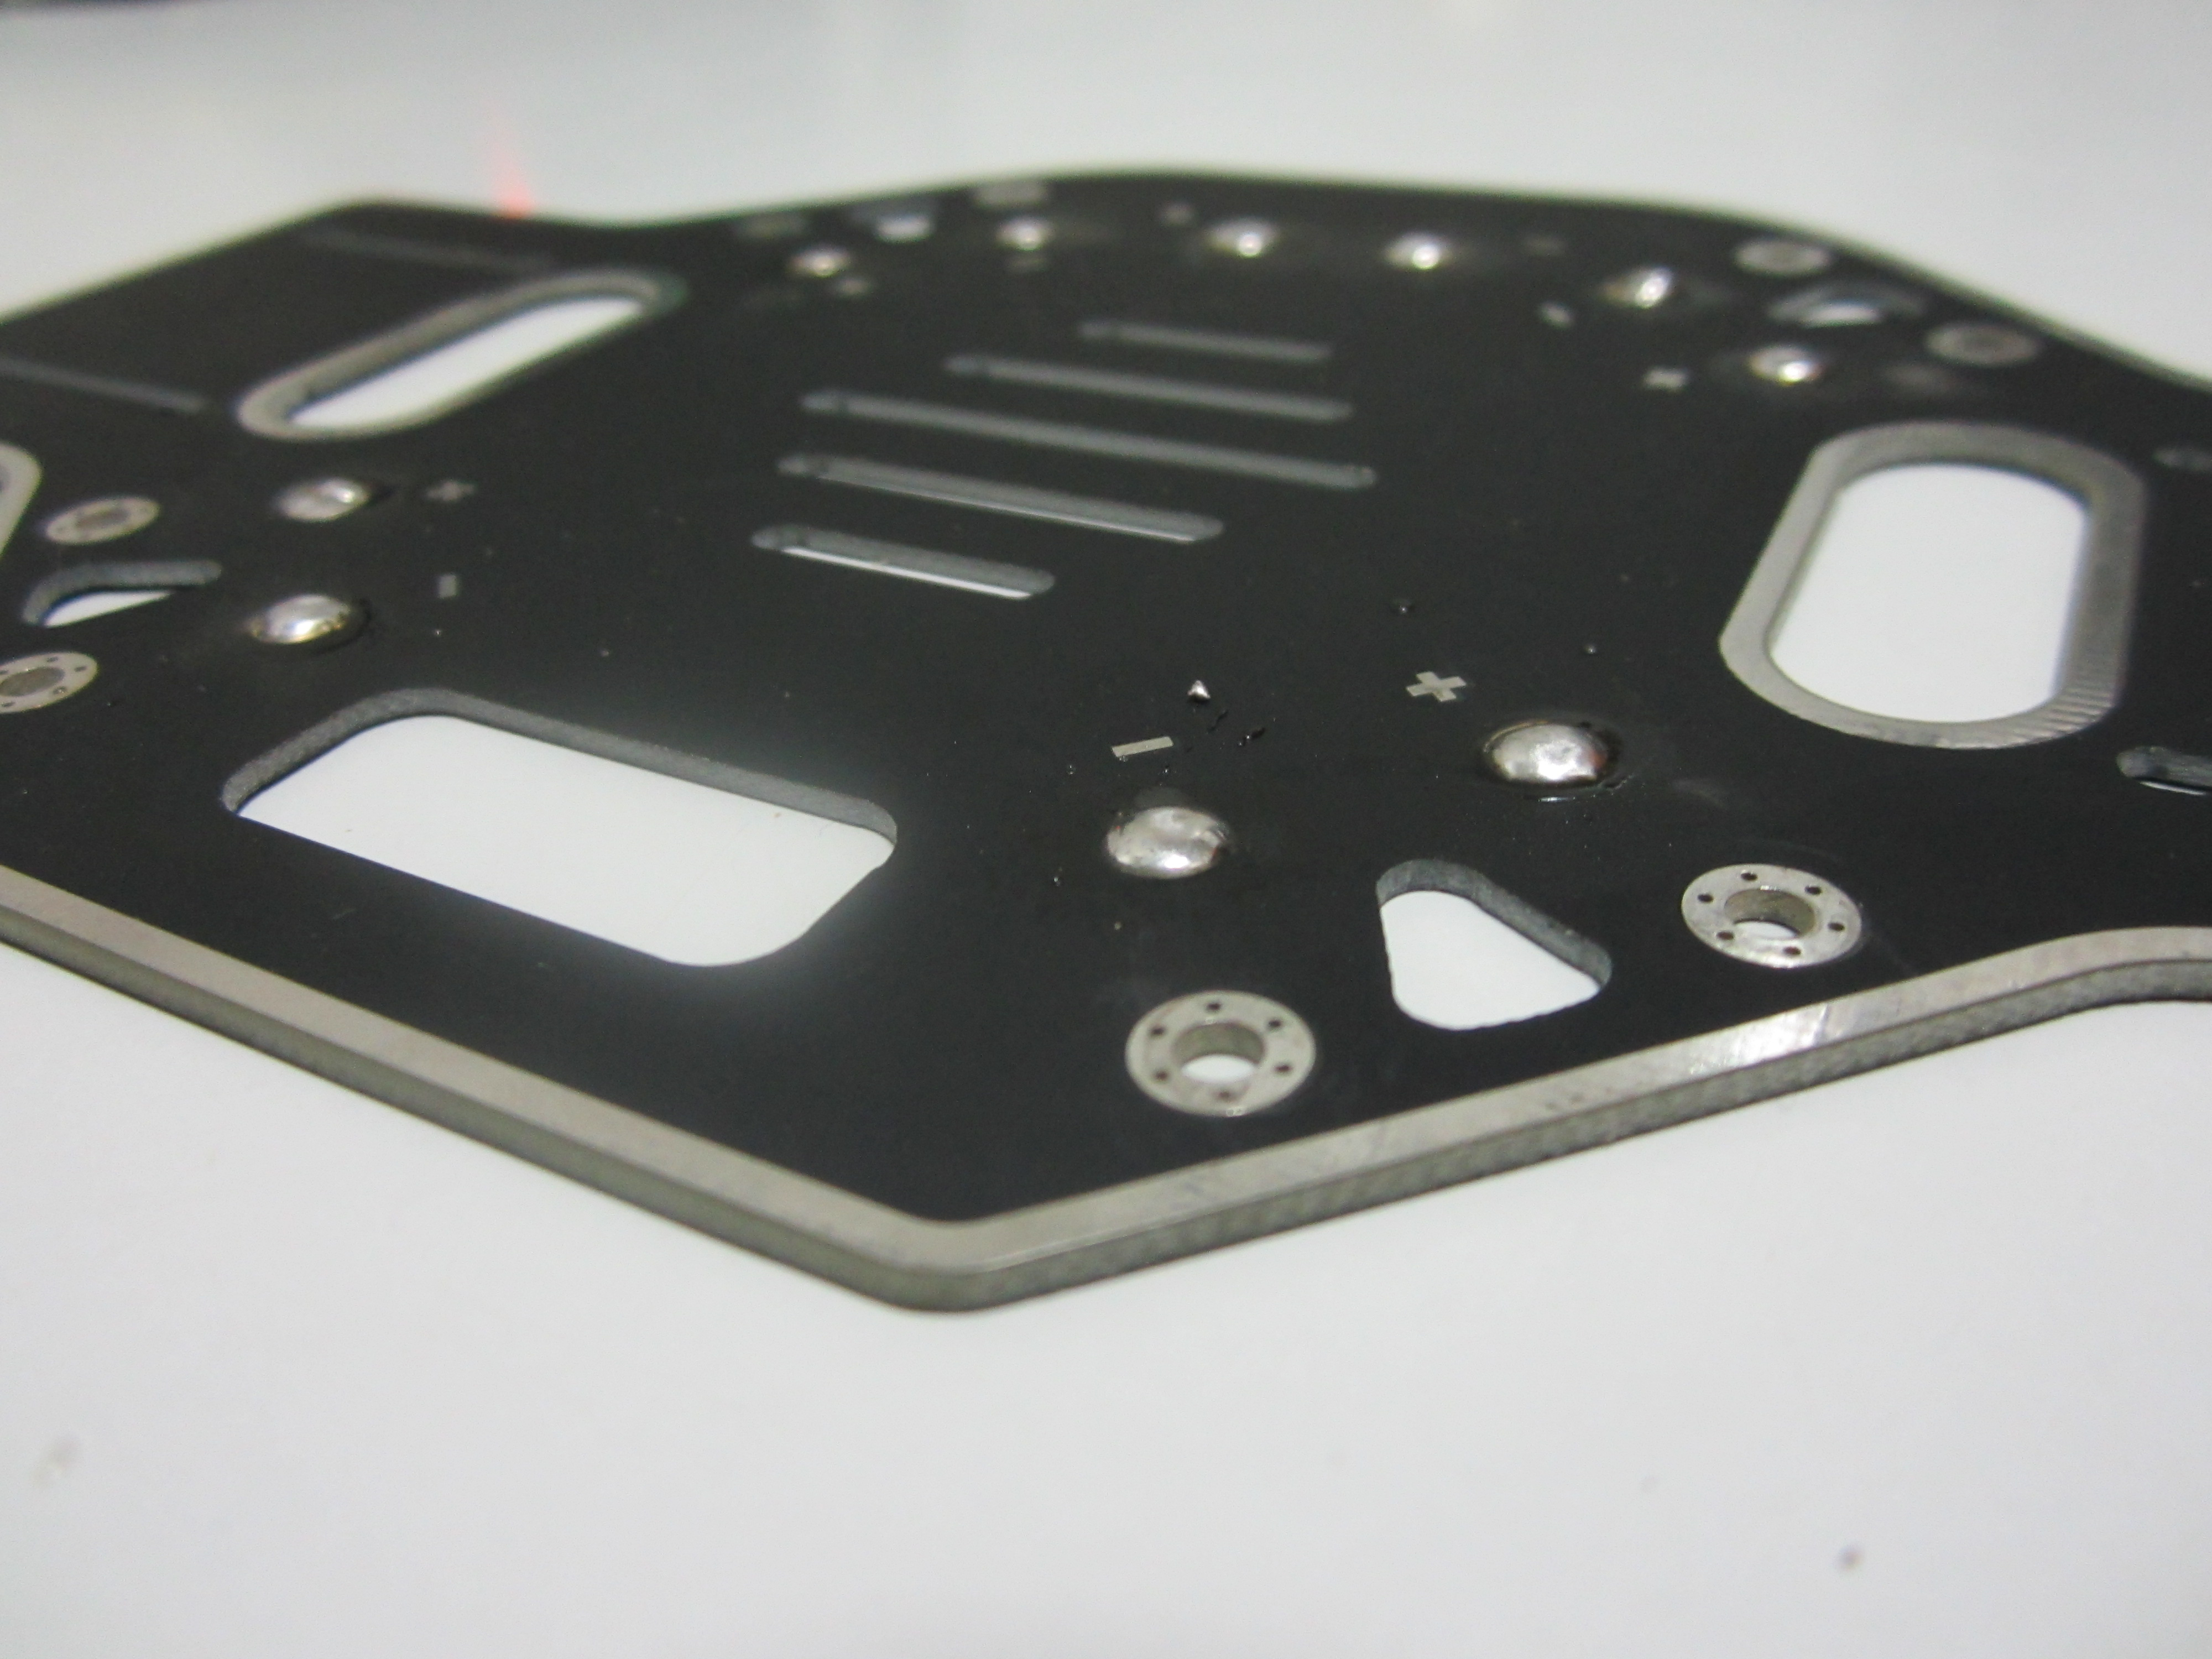
\includegraphics[width=0.8\linewidth]{Images/Mounting/IMG_0374.jpg}
  \captionof{figure}{}
  \label{fig:app2}
\end{minipage}
\\[12 pt]

\begin{minipage}{0.5\textwidth}
  \centering
  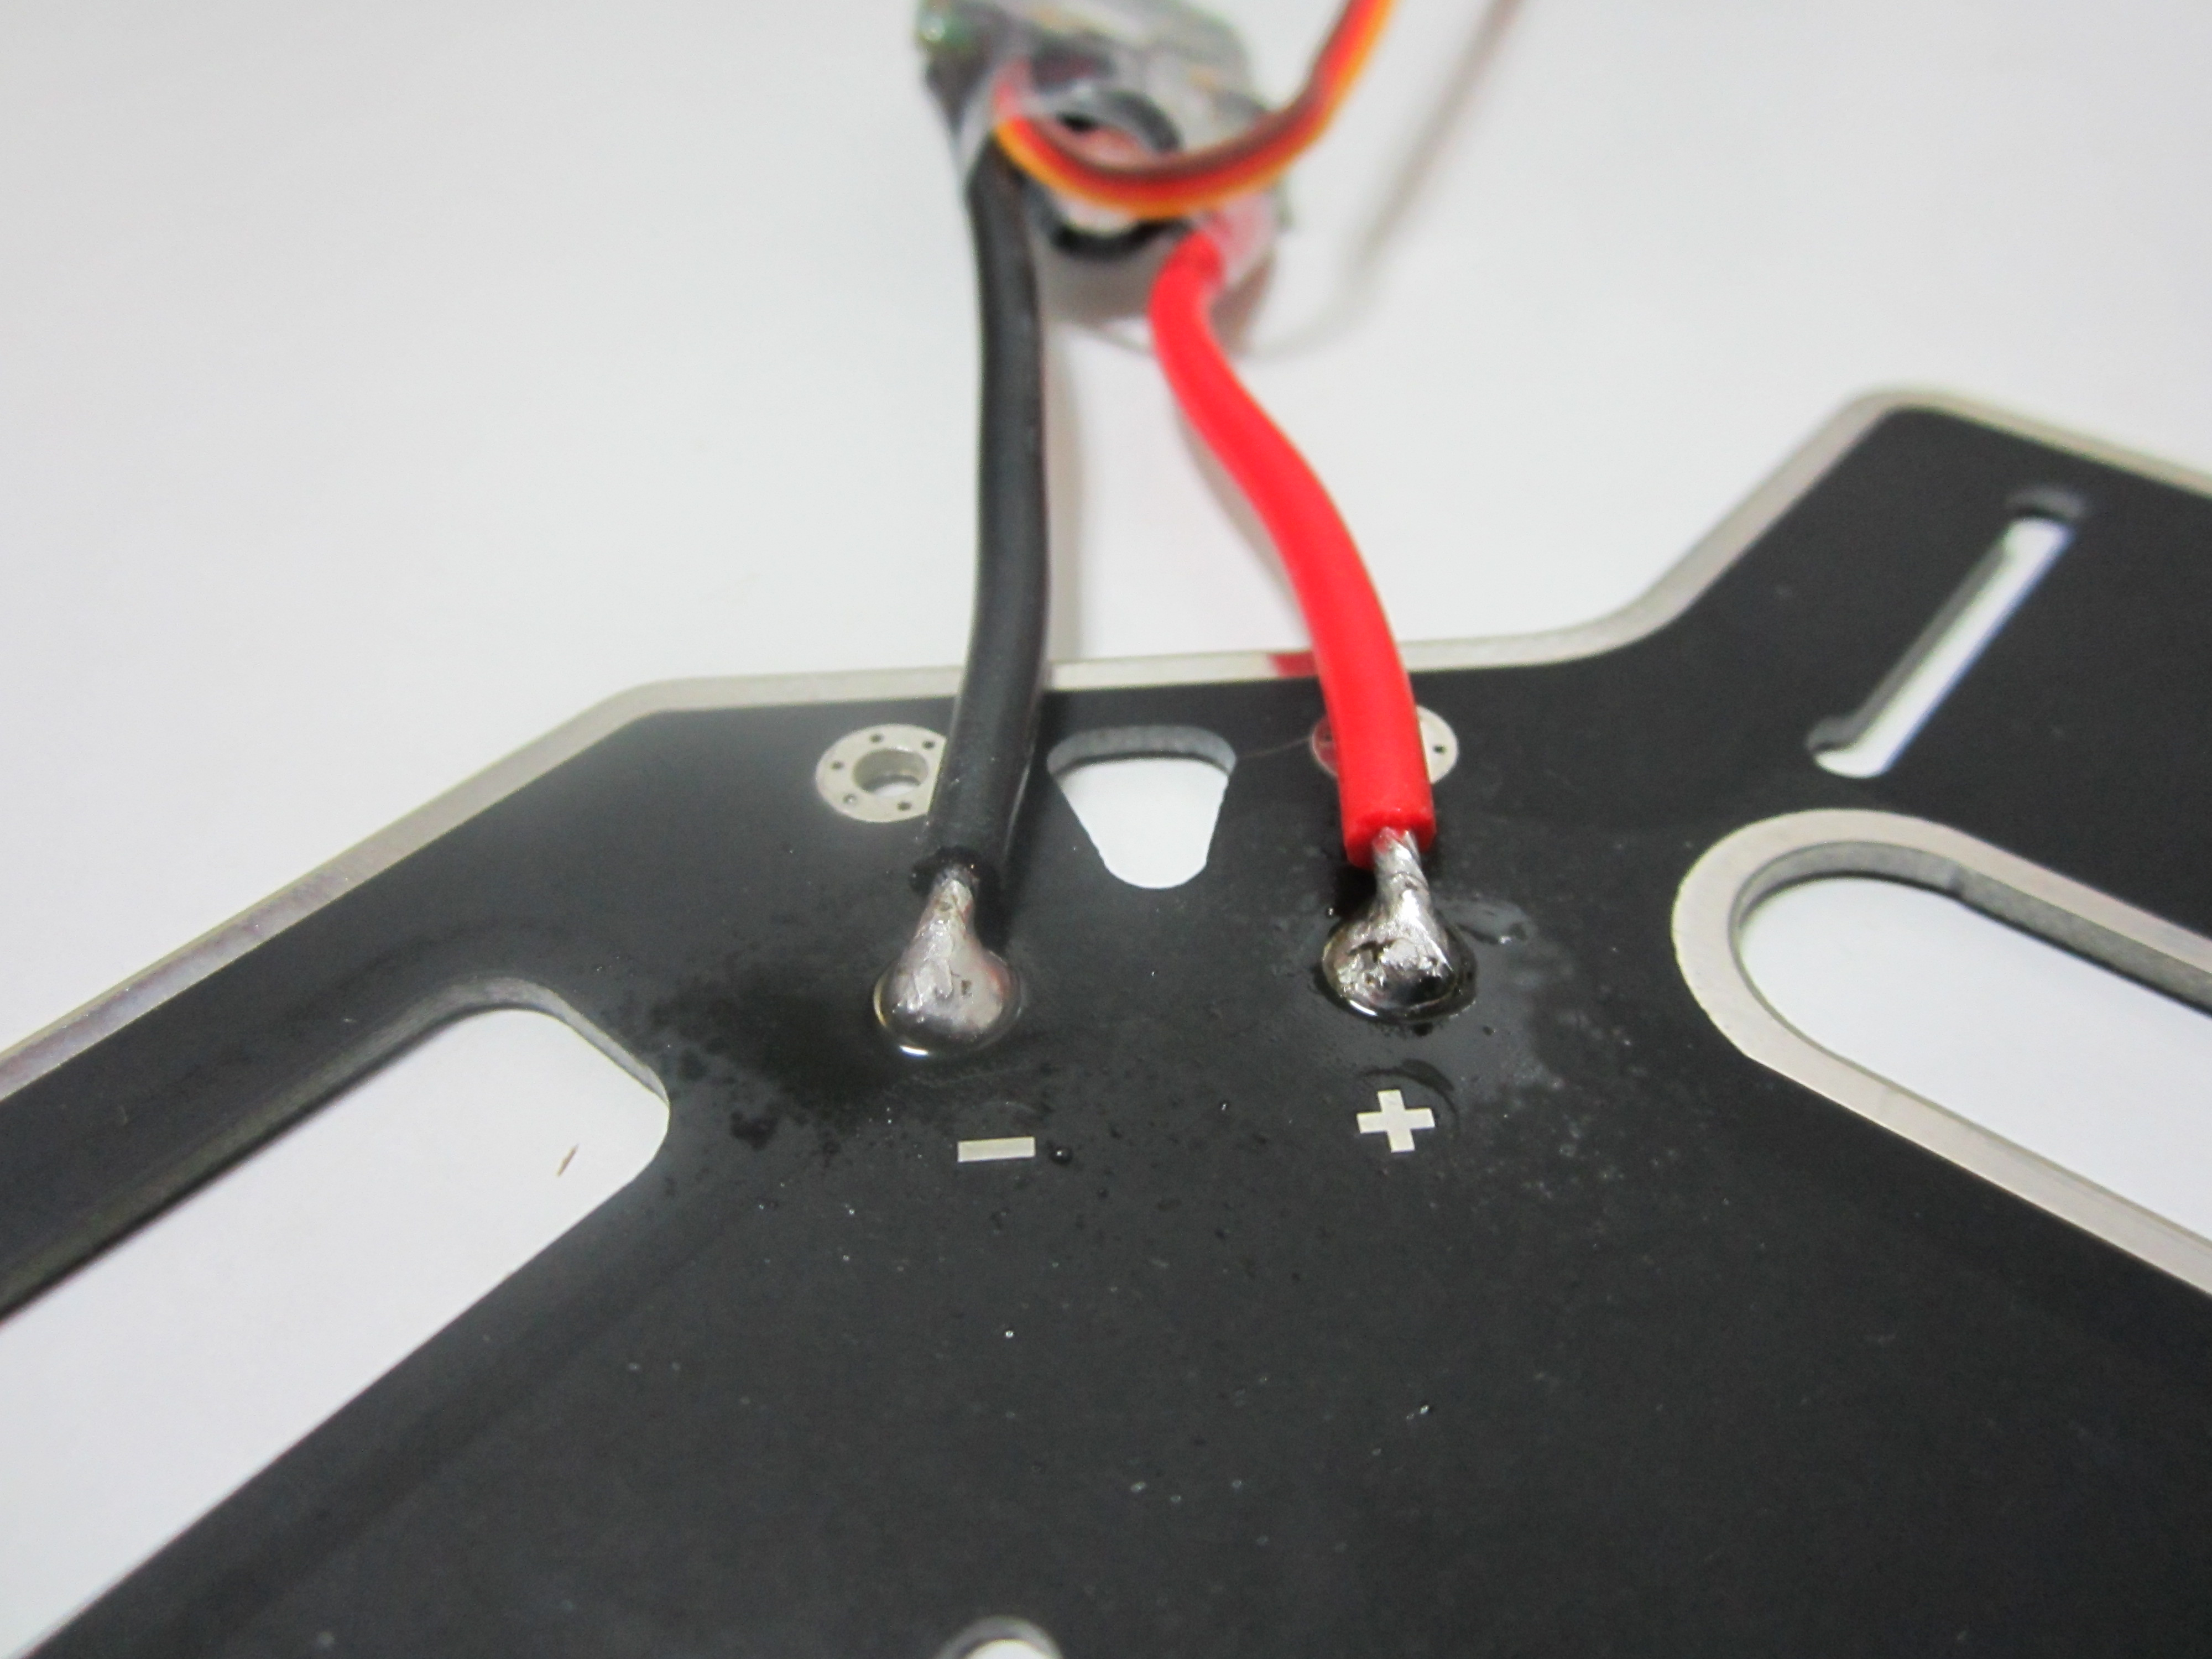
\includegraphics[width=0.8\linewidth]{Images/Mounting/IMG_0379.jpg}
  \captionof{figure}{}
  \label{fig:app1}
\end{minipage}%
\begin{minipage}{0.5\textwidth}
  \centering
  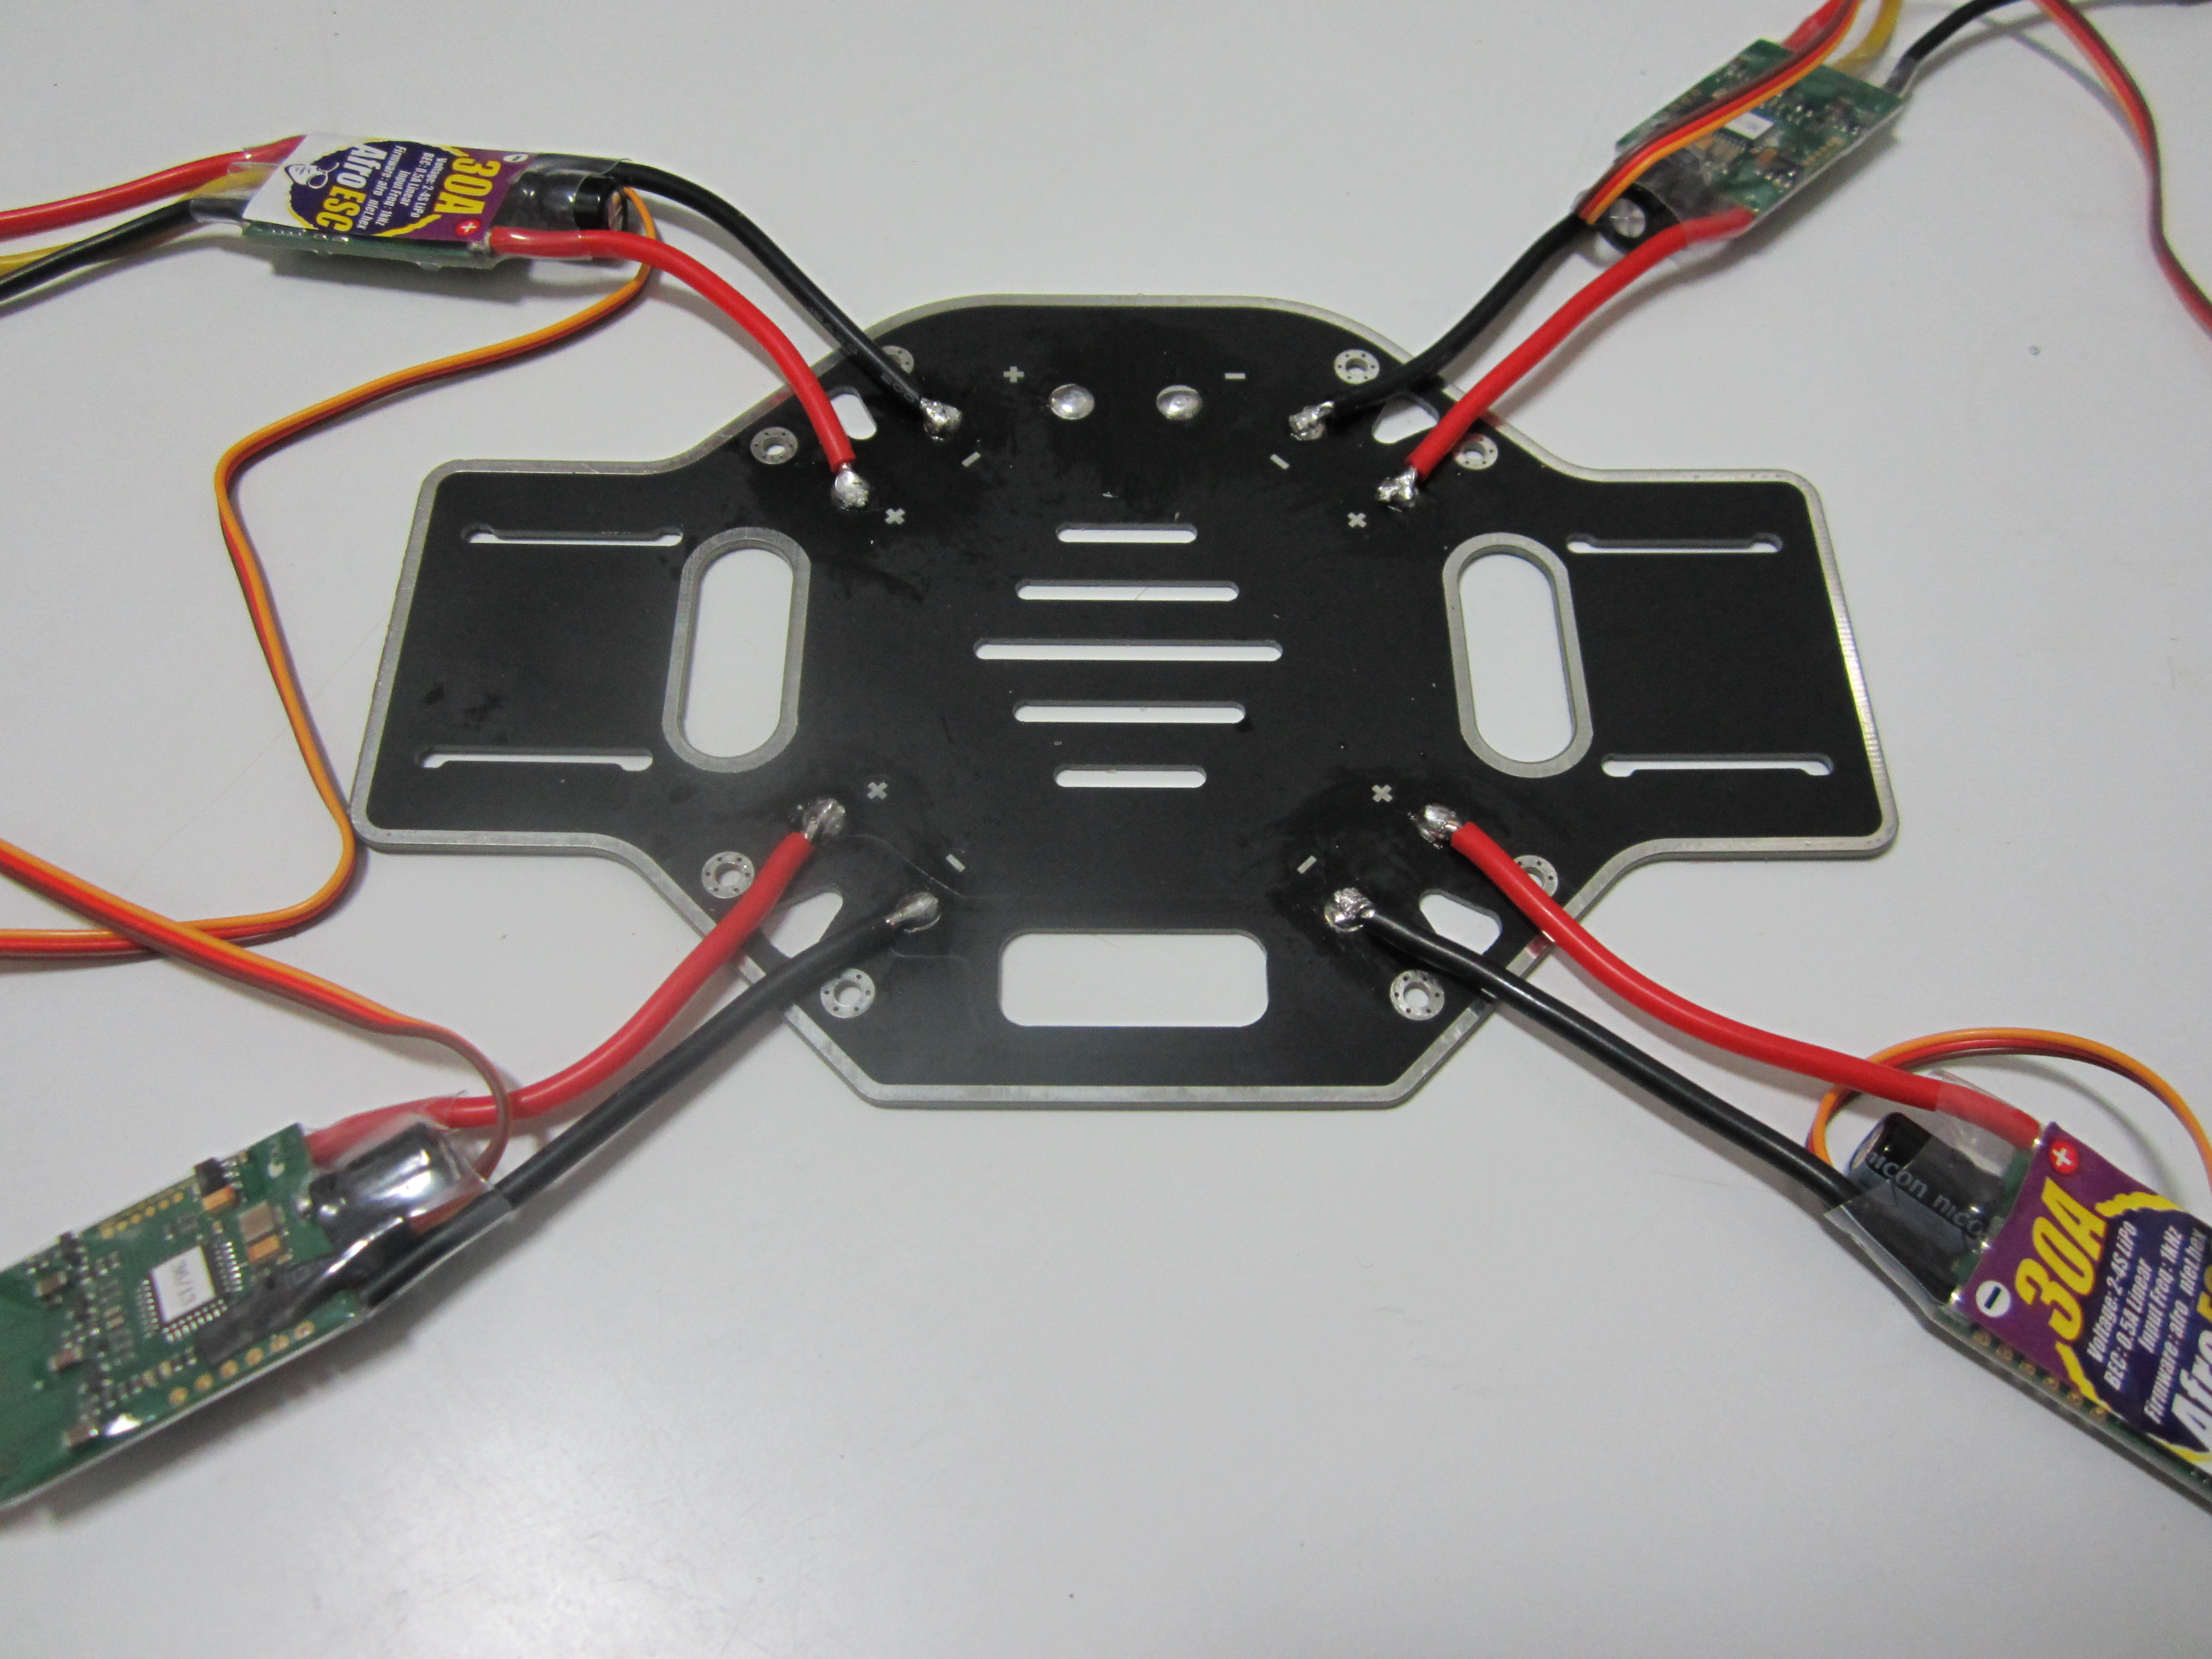
\includegraphics[width=0.8\linewidth]{Images/Mounting/IMG_0384.jpg}
  \captionof{figure}{}
  \label{fig:app2}
\end{minipage}
\\[12pt]


Once the ESCs have been soldered at the base, it is time to solder the cables that connect to the battery. These cables were purchased aside with a series of connectors compatible with the battery in order to build the necessary wiring.

To find out the length of the cable that connects to the battery is recommended to simulate the assembly of the infrastructure with the arms and putting the battery in the top base to see how this connects with the cables.
\\[12 pt]

\begin{minipage}{0.5\textwidth}
  \centering
  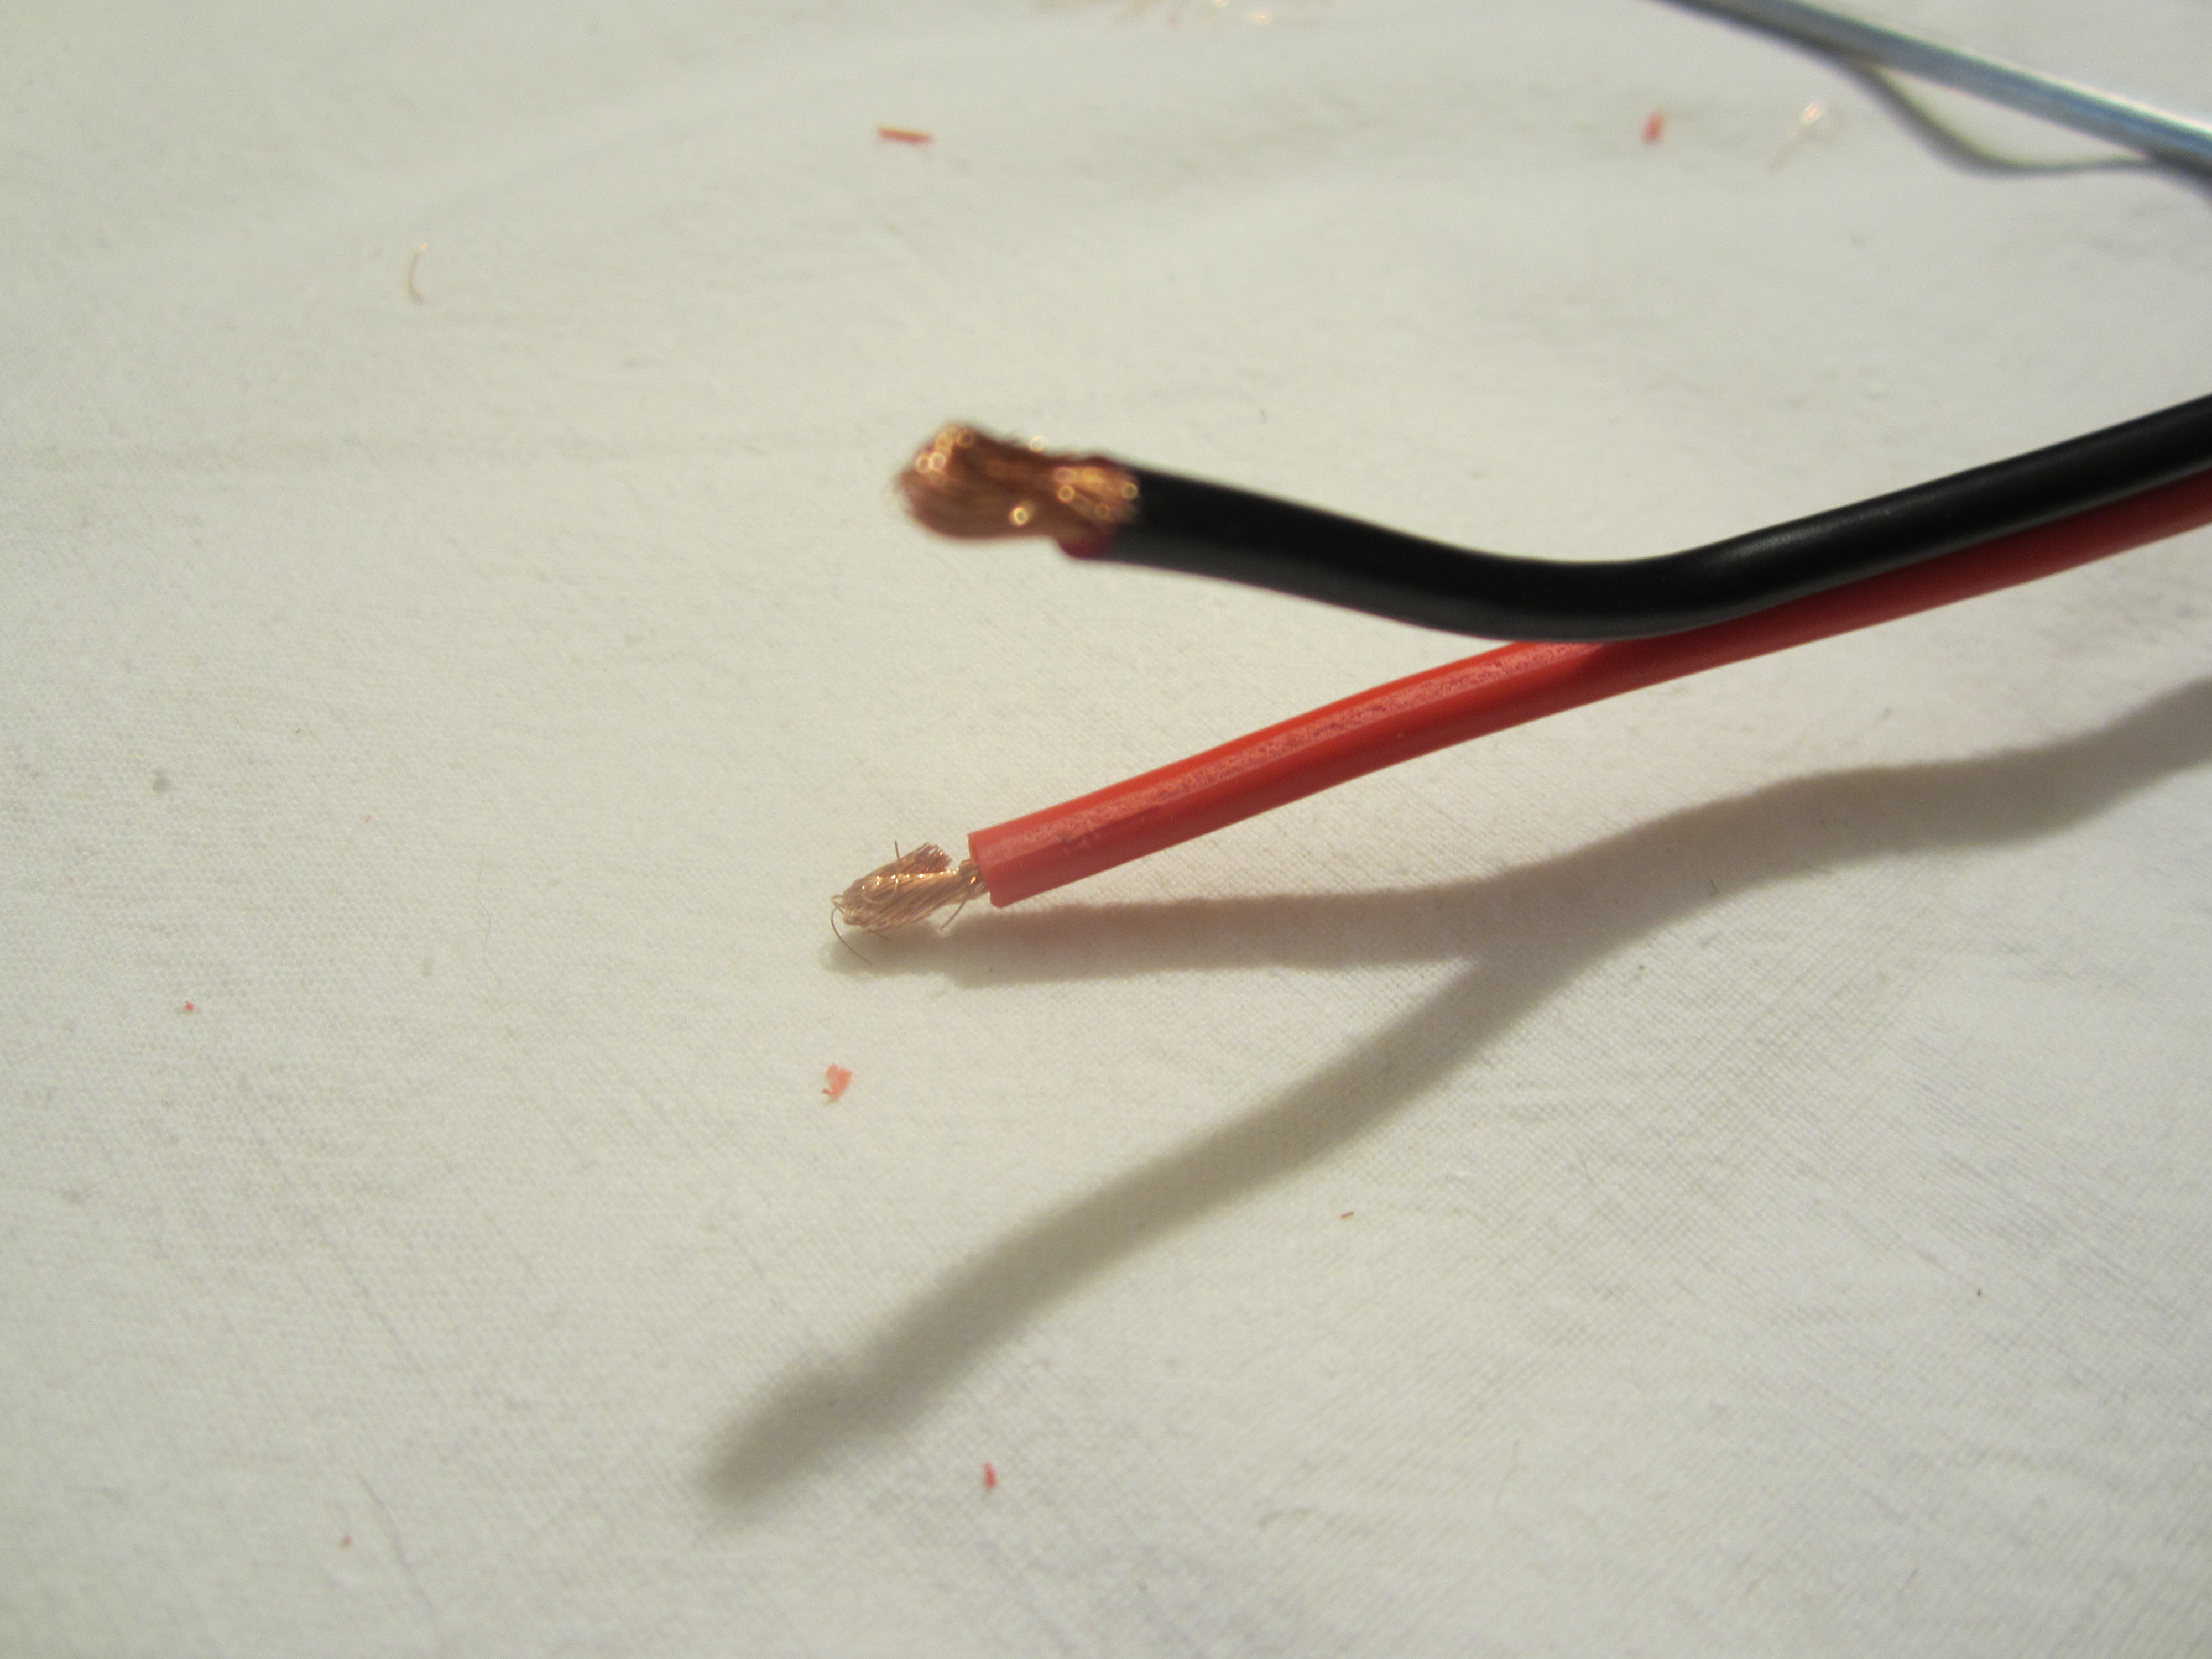
\includegraphics[width=0.8\linewidth]{Images/Mounting/IMG_0385.jpg}
  \captionof{figure}{}
  \label{fig:app1}
\end{minipage}%
\begin{minipage}{0.5\textwidth}
  \centering
  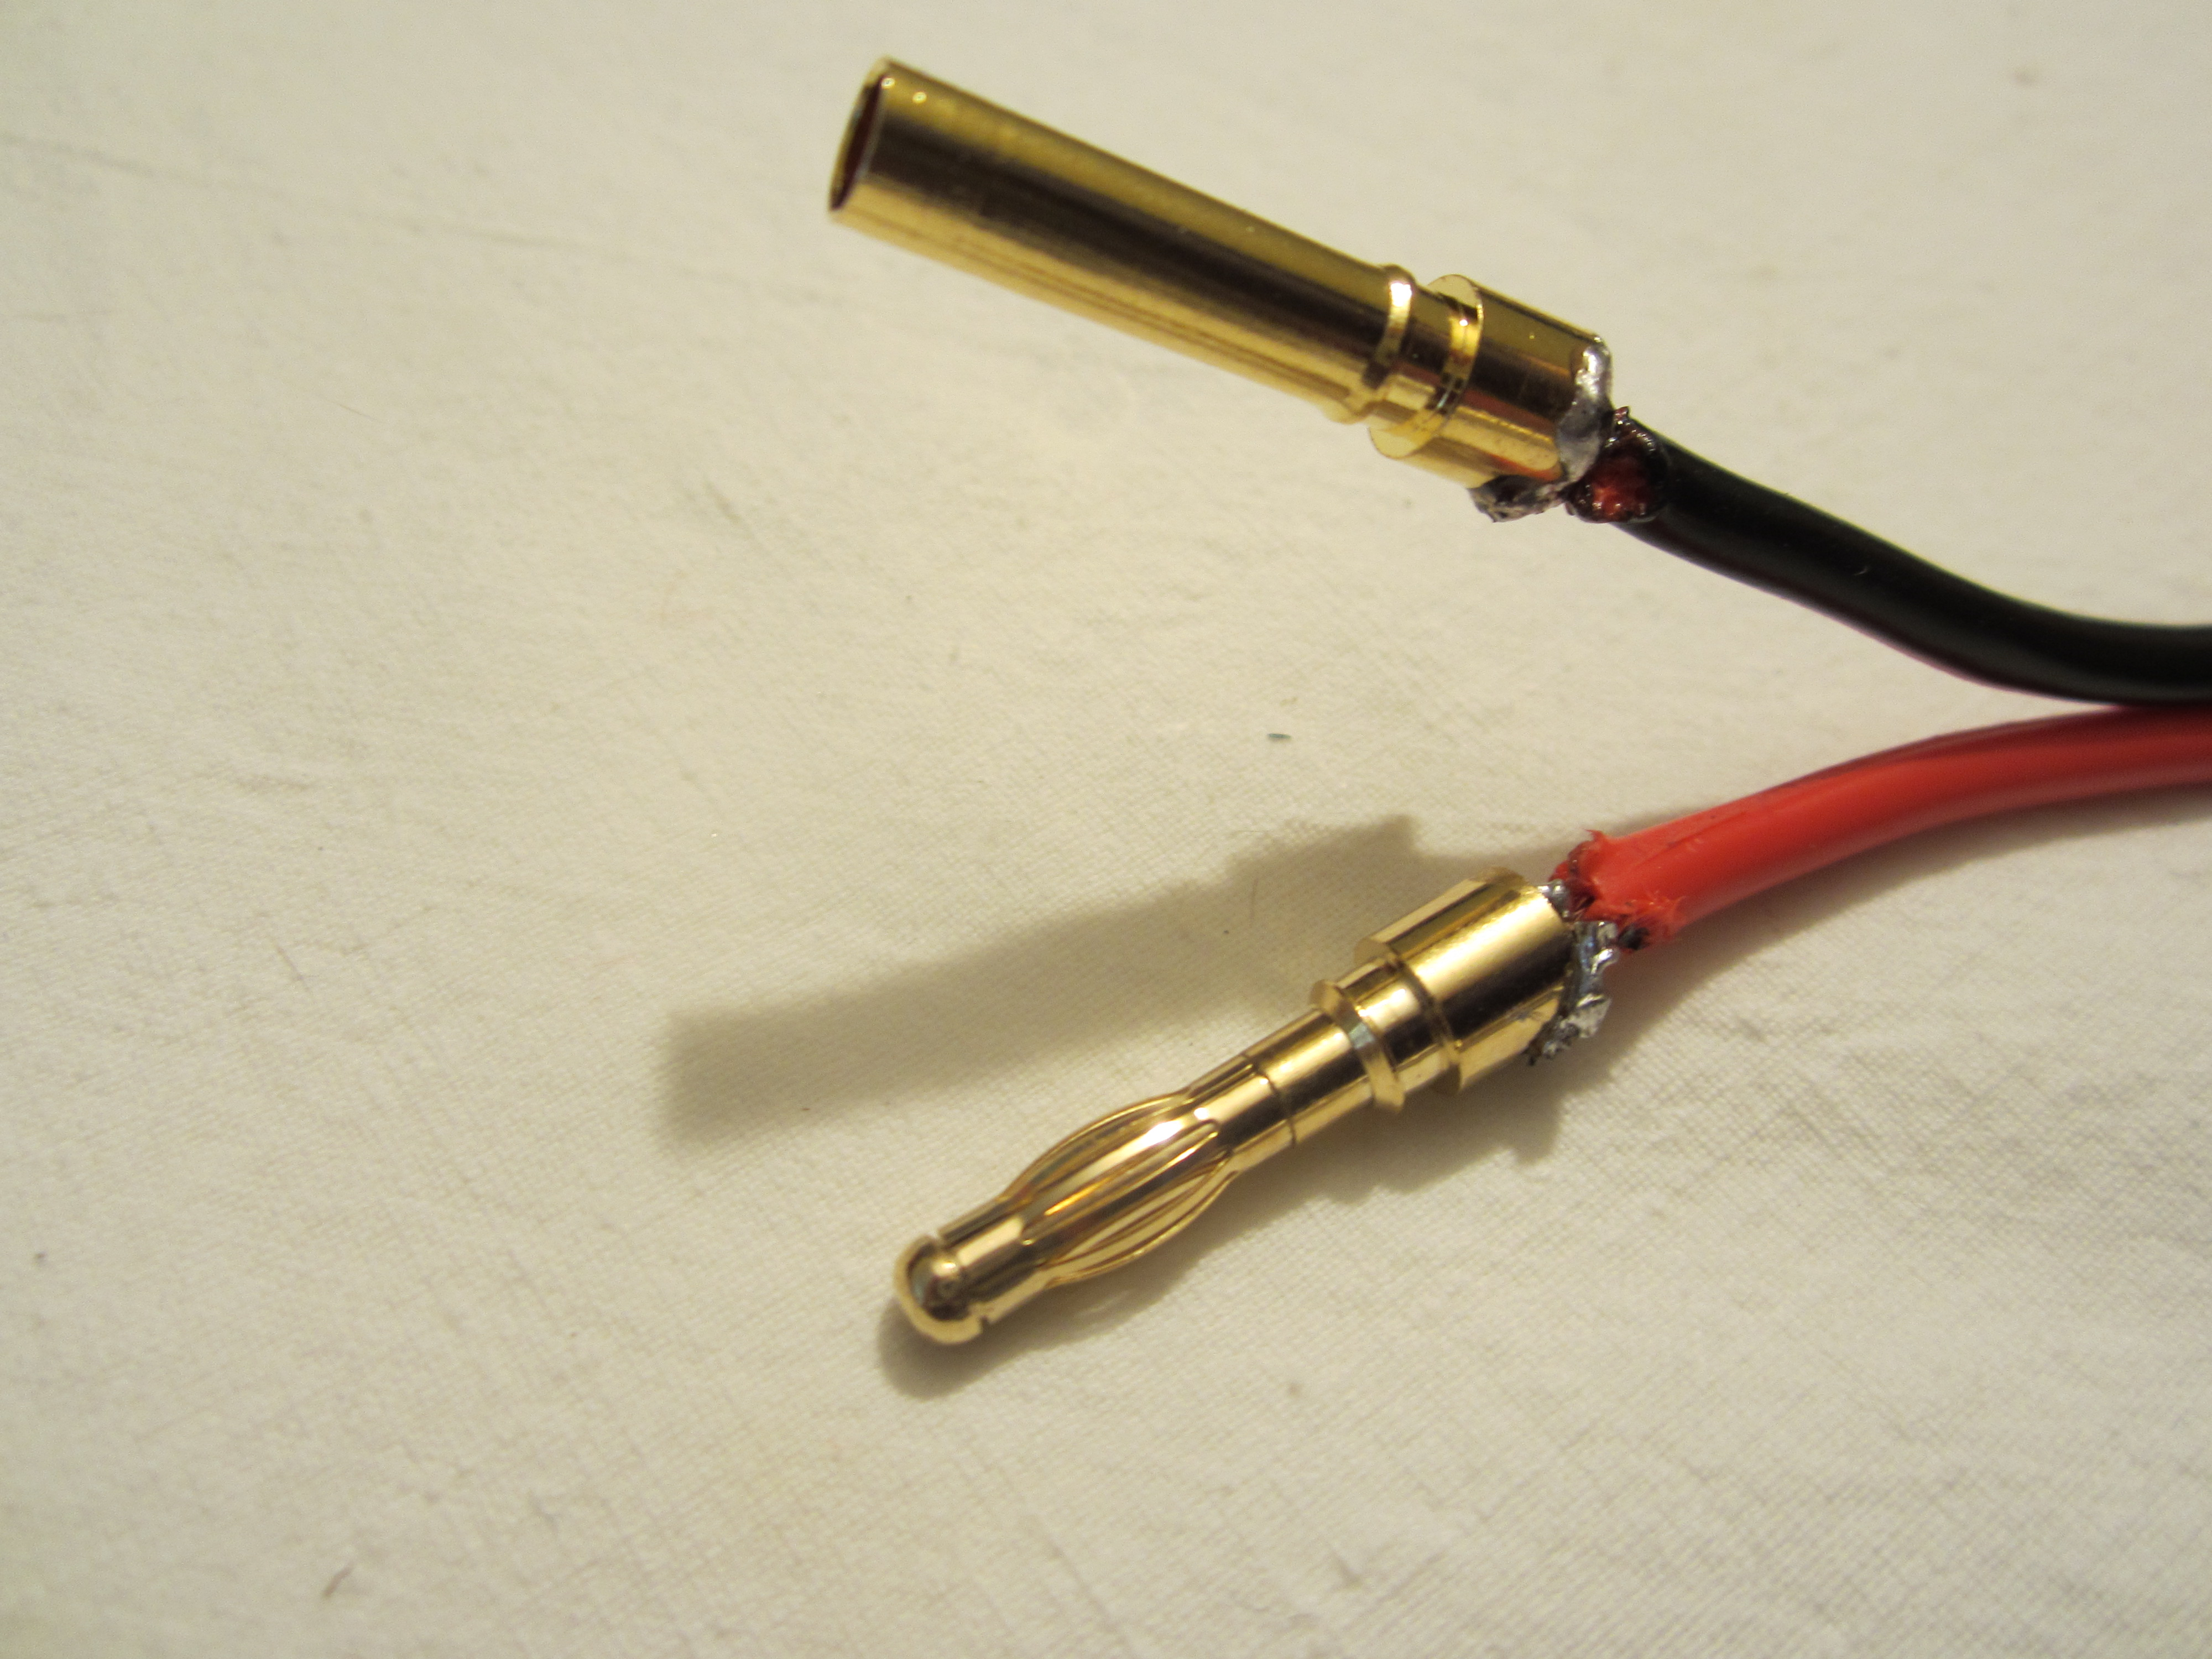
\includegraphics[width=0.8\linewidth]{Images/Mounting/IMG_0390.jpg}
  \captionof{figure}{}
  \label{fig:app2}
\end{minipage}
\\[12pt]

\begin{minipage}{0.5\textwidth}
  \centering
  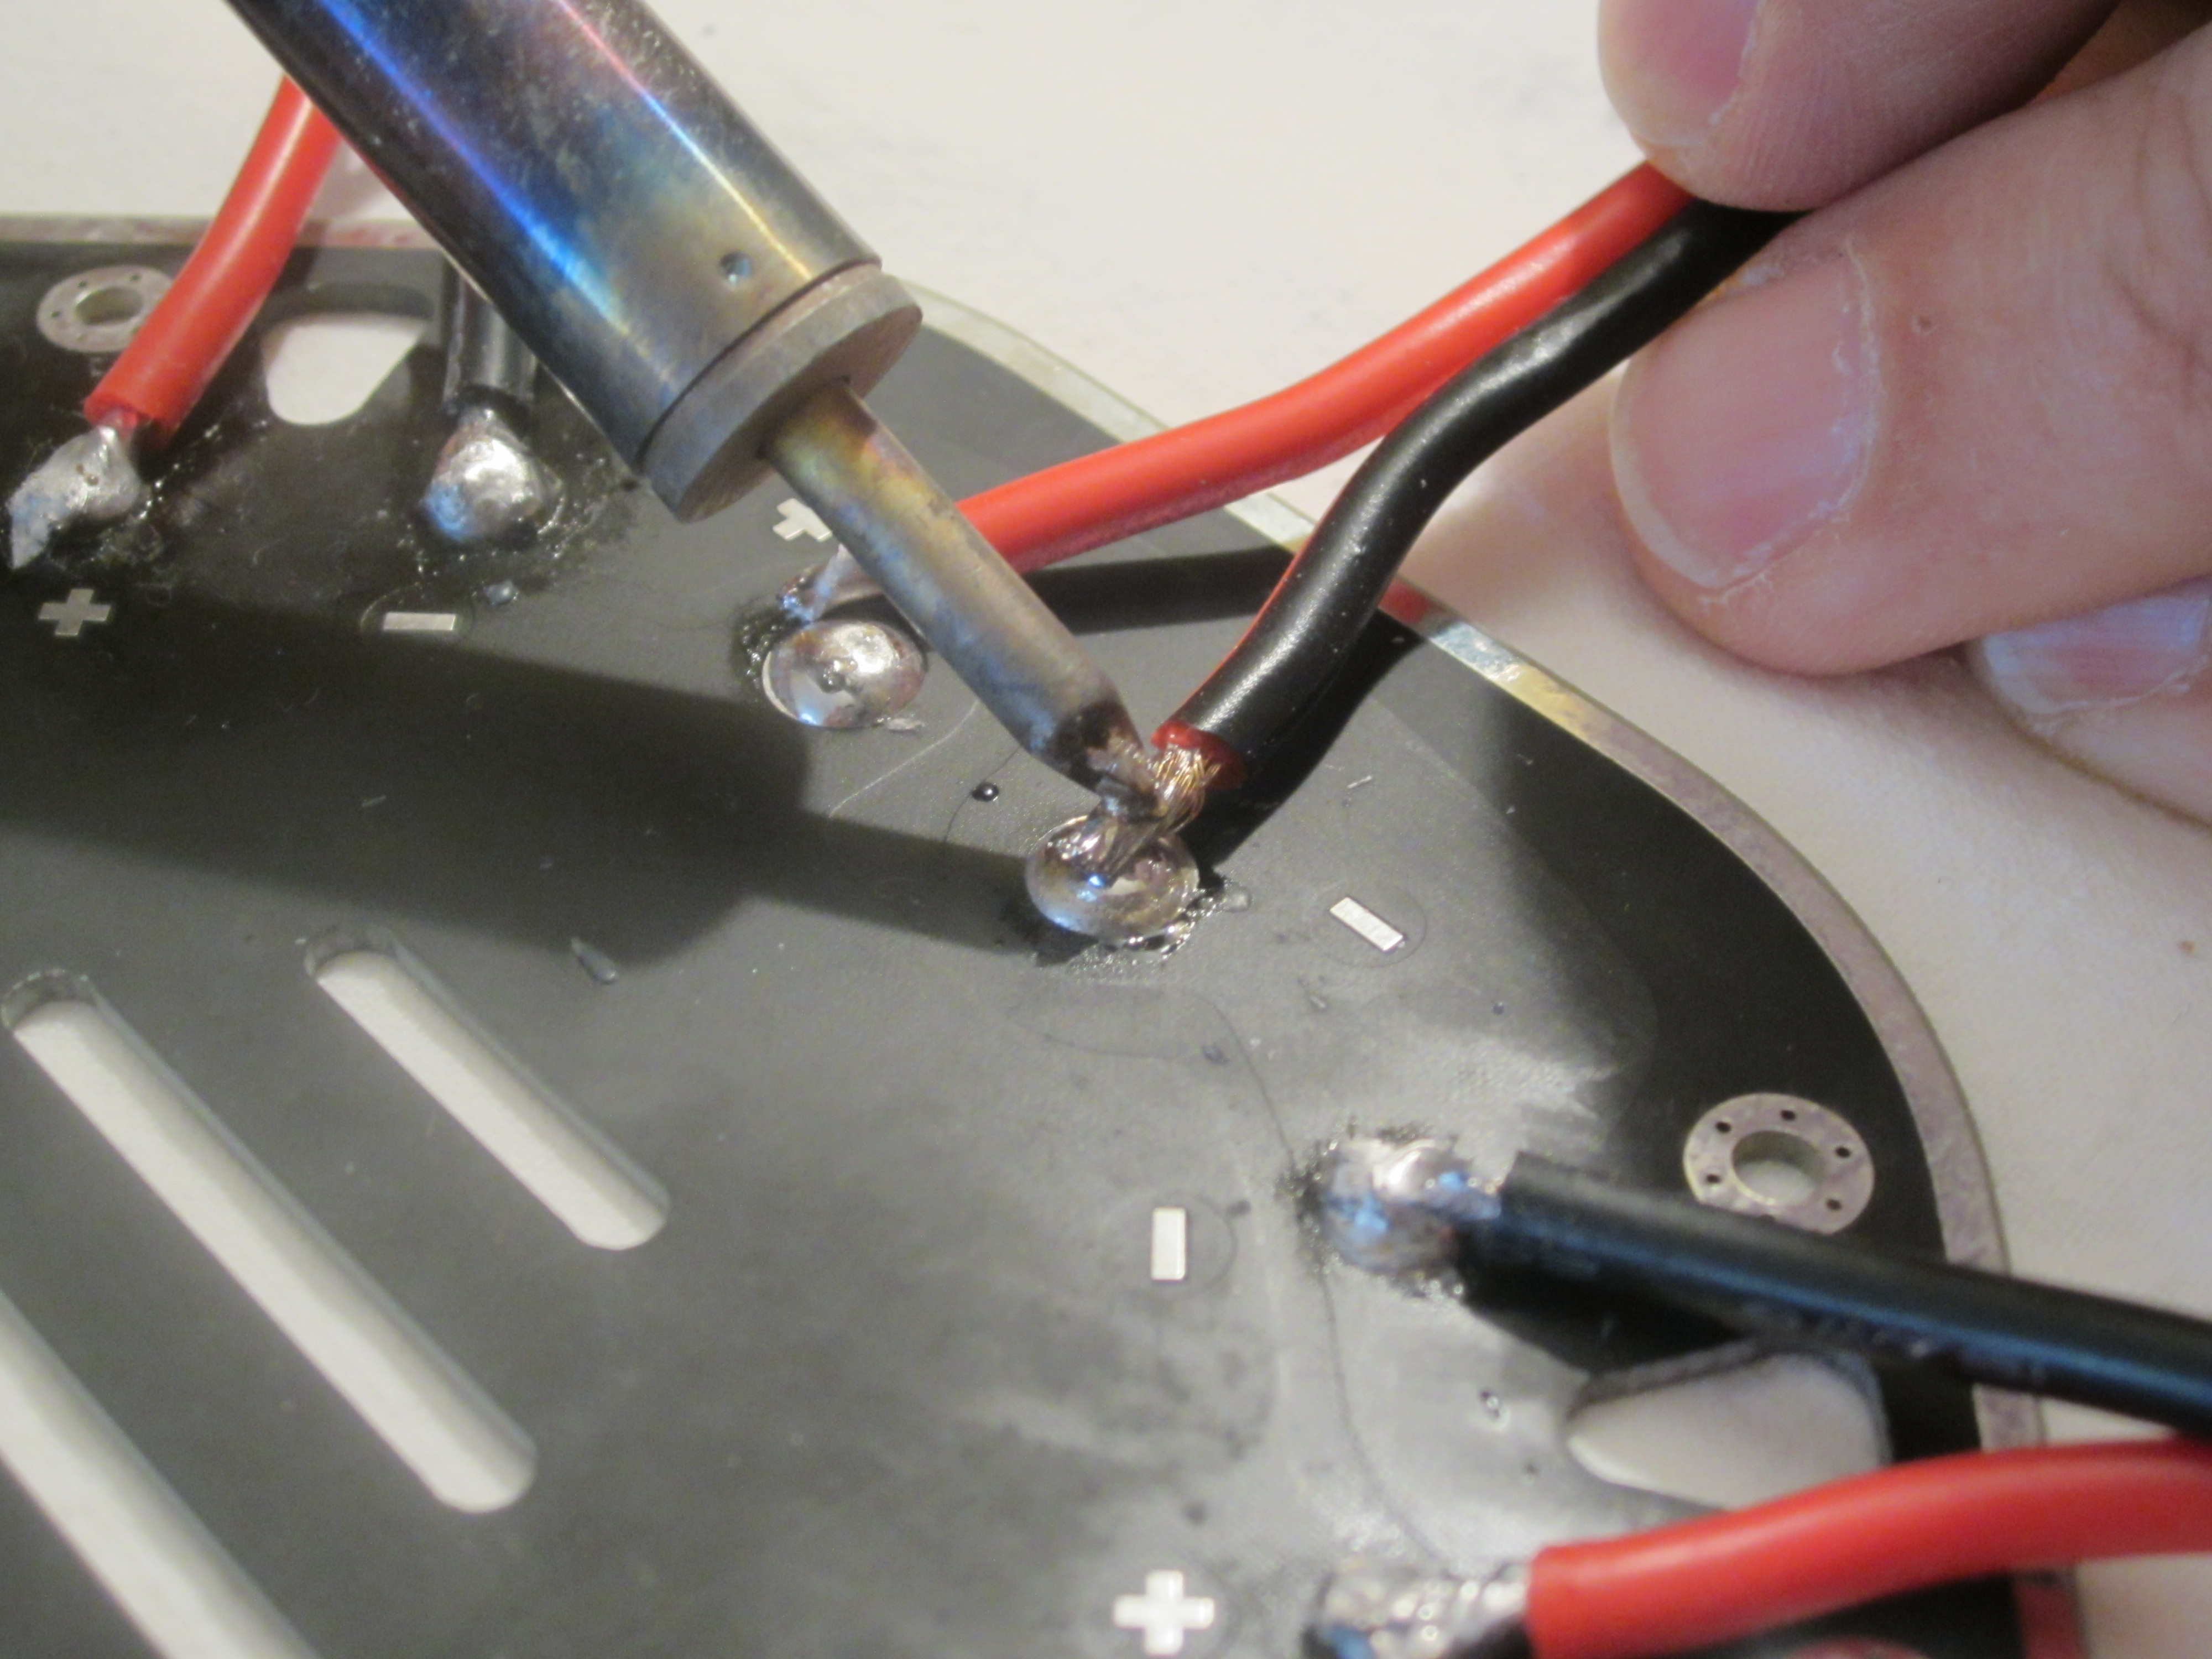
\includegraphics[width=0.8\linewidth]{Images/Mounting/IMG_0392.jpg}
  \captionof{figure}{}
  \label{fig:app1}
\end{minipage}%
\begin{minipage}{0.5\textwidth}
  \centering
  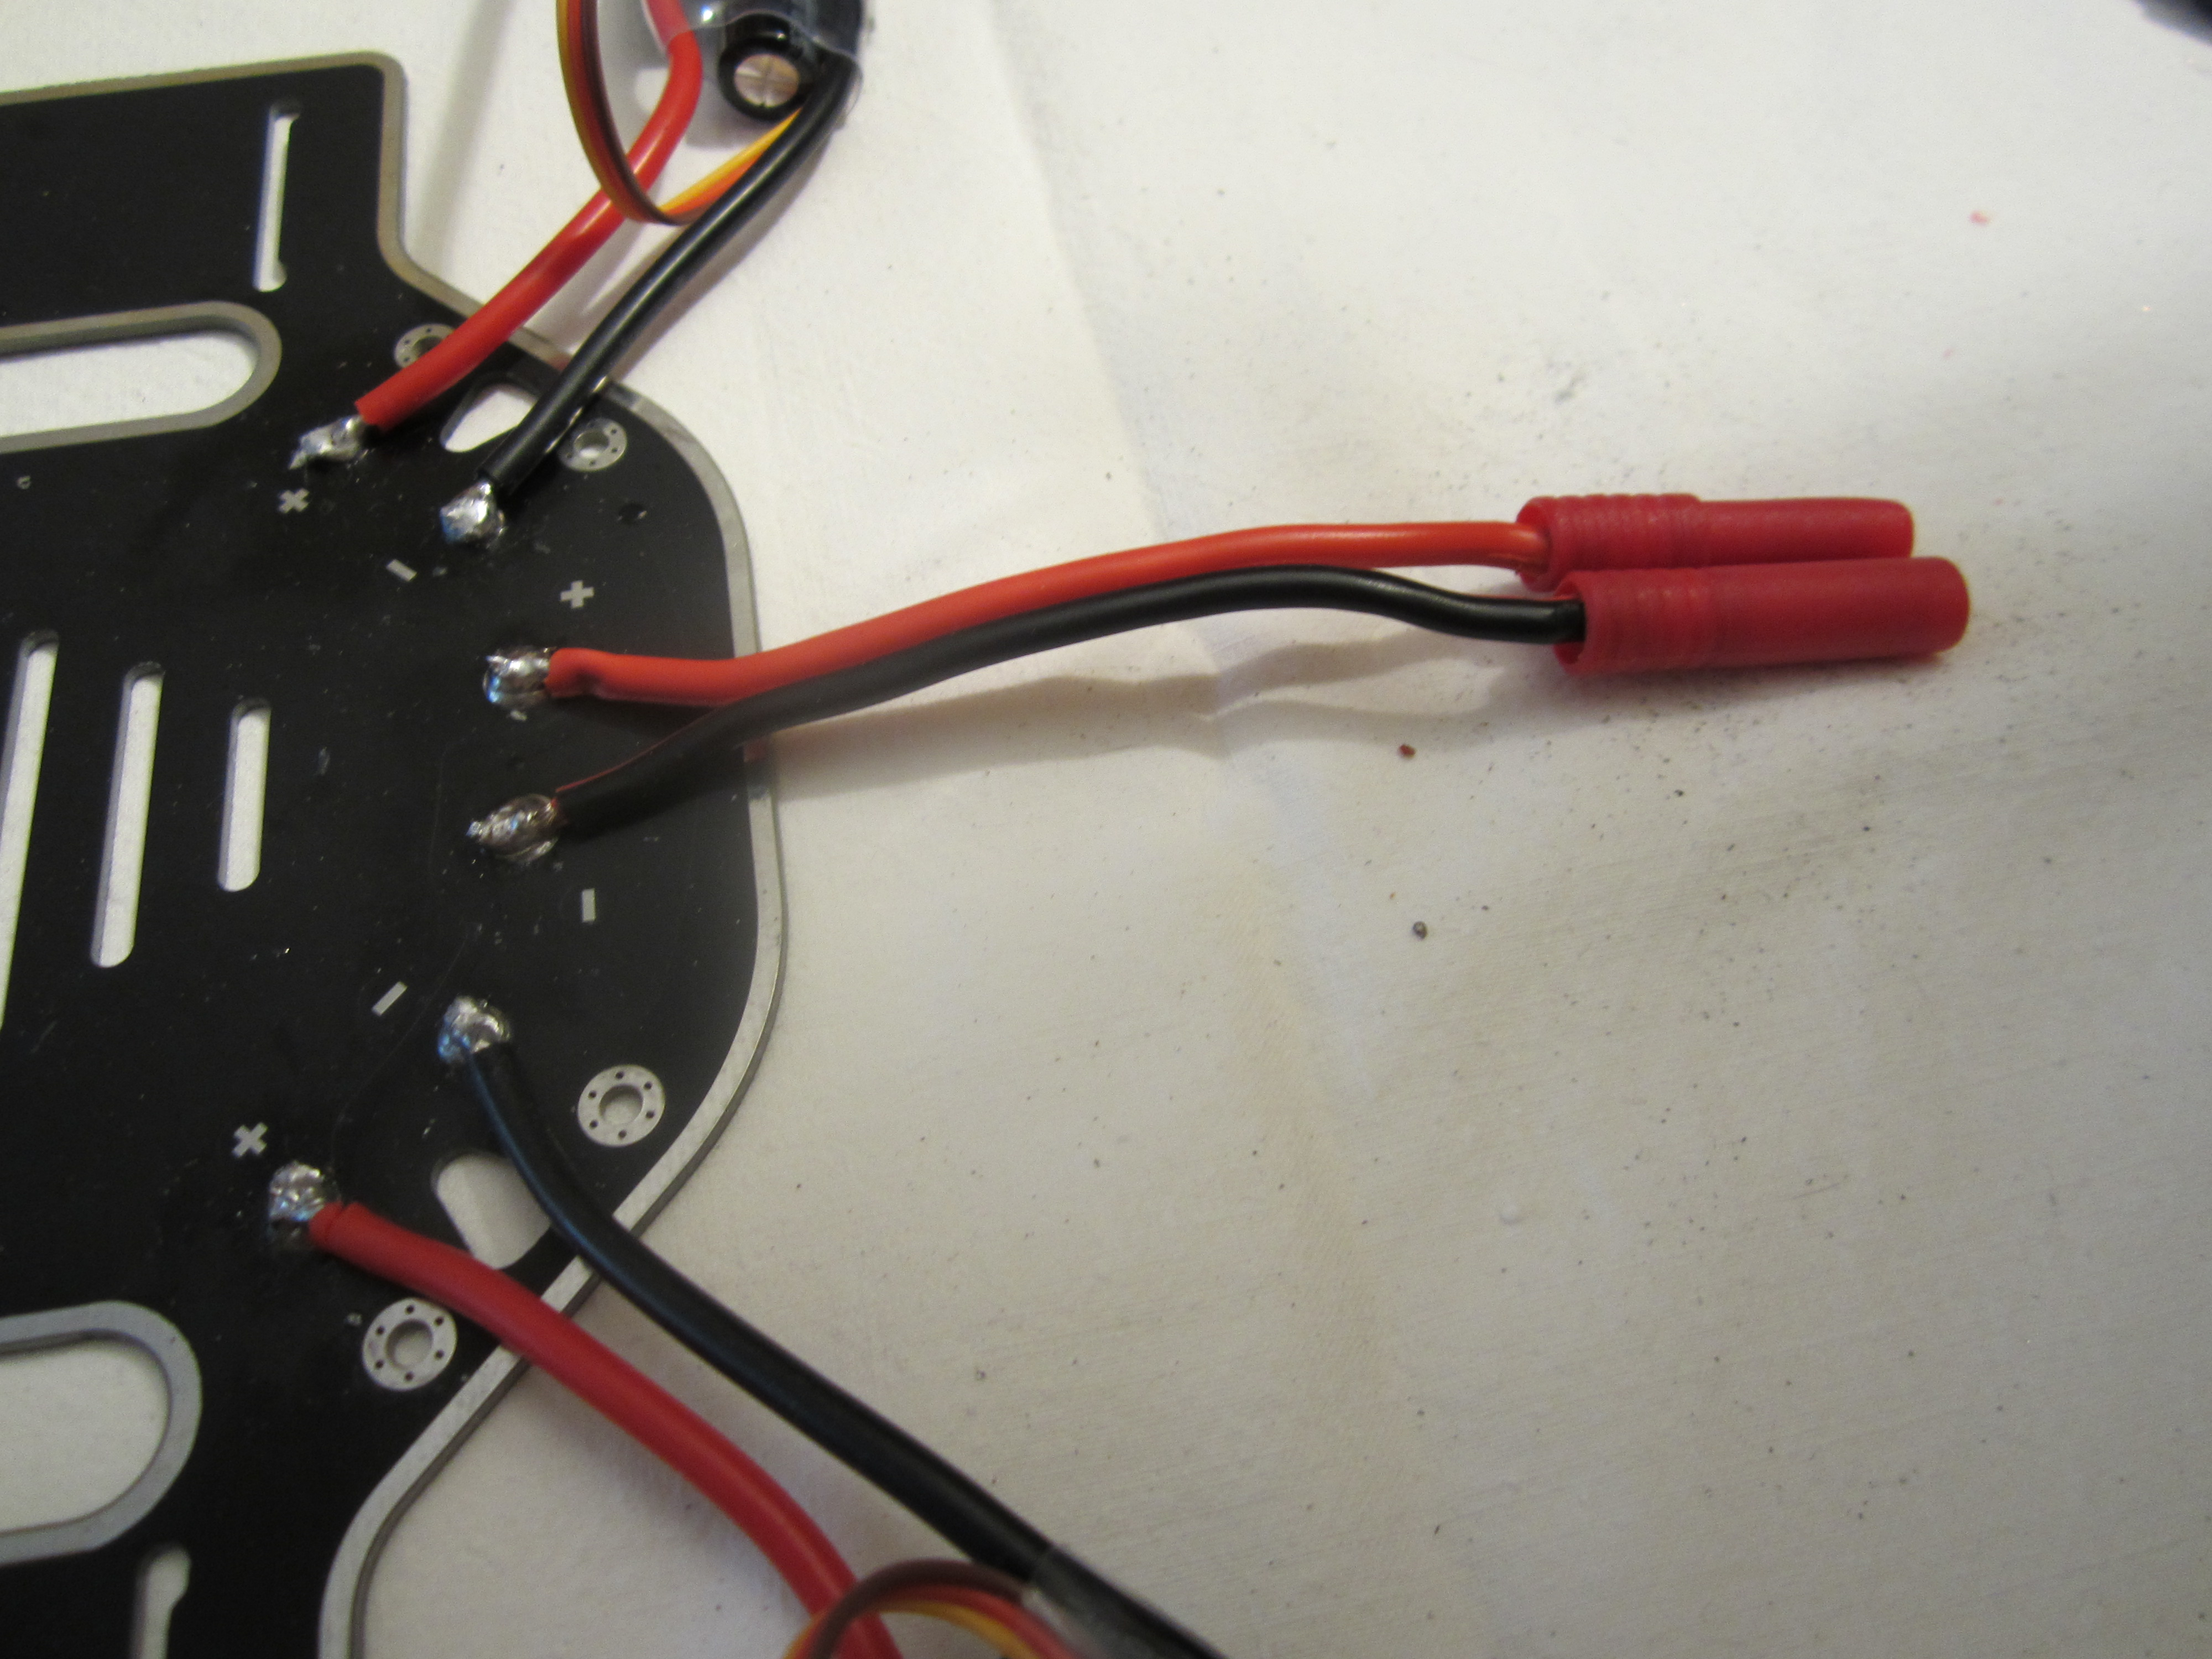
\includegraphics[width=0.8\linewidth]{Images/Mounting/IMG_0394.jpg}
  \captionof{figure}{}
  \label{fig:app2}
\end{minipage}
\\[12pt]

Once you have all the welding done, it is advisable to apply a bit of silicone with a cold gun to protect these points and avoid possible short circuits later.

\begin{minipage}{0.5\textwidth}
  \centering
  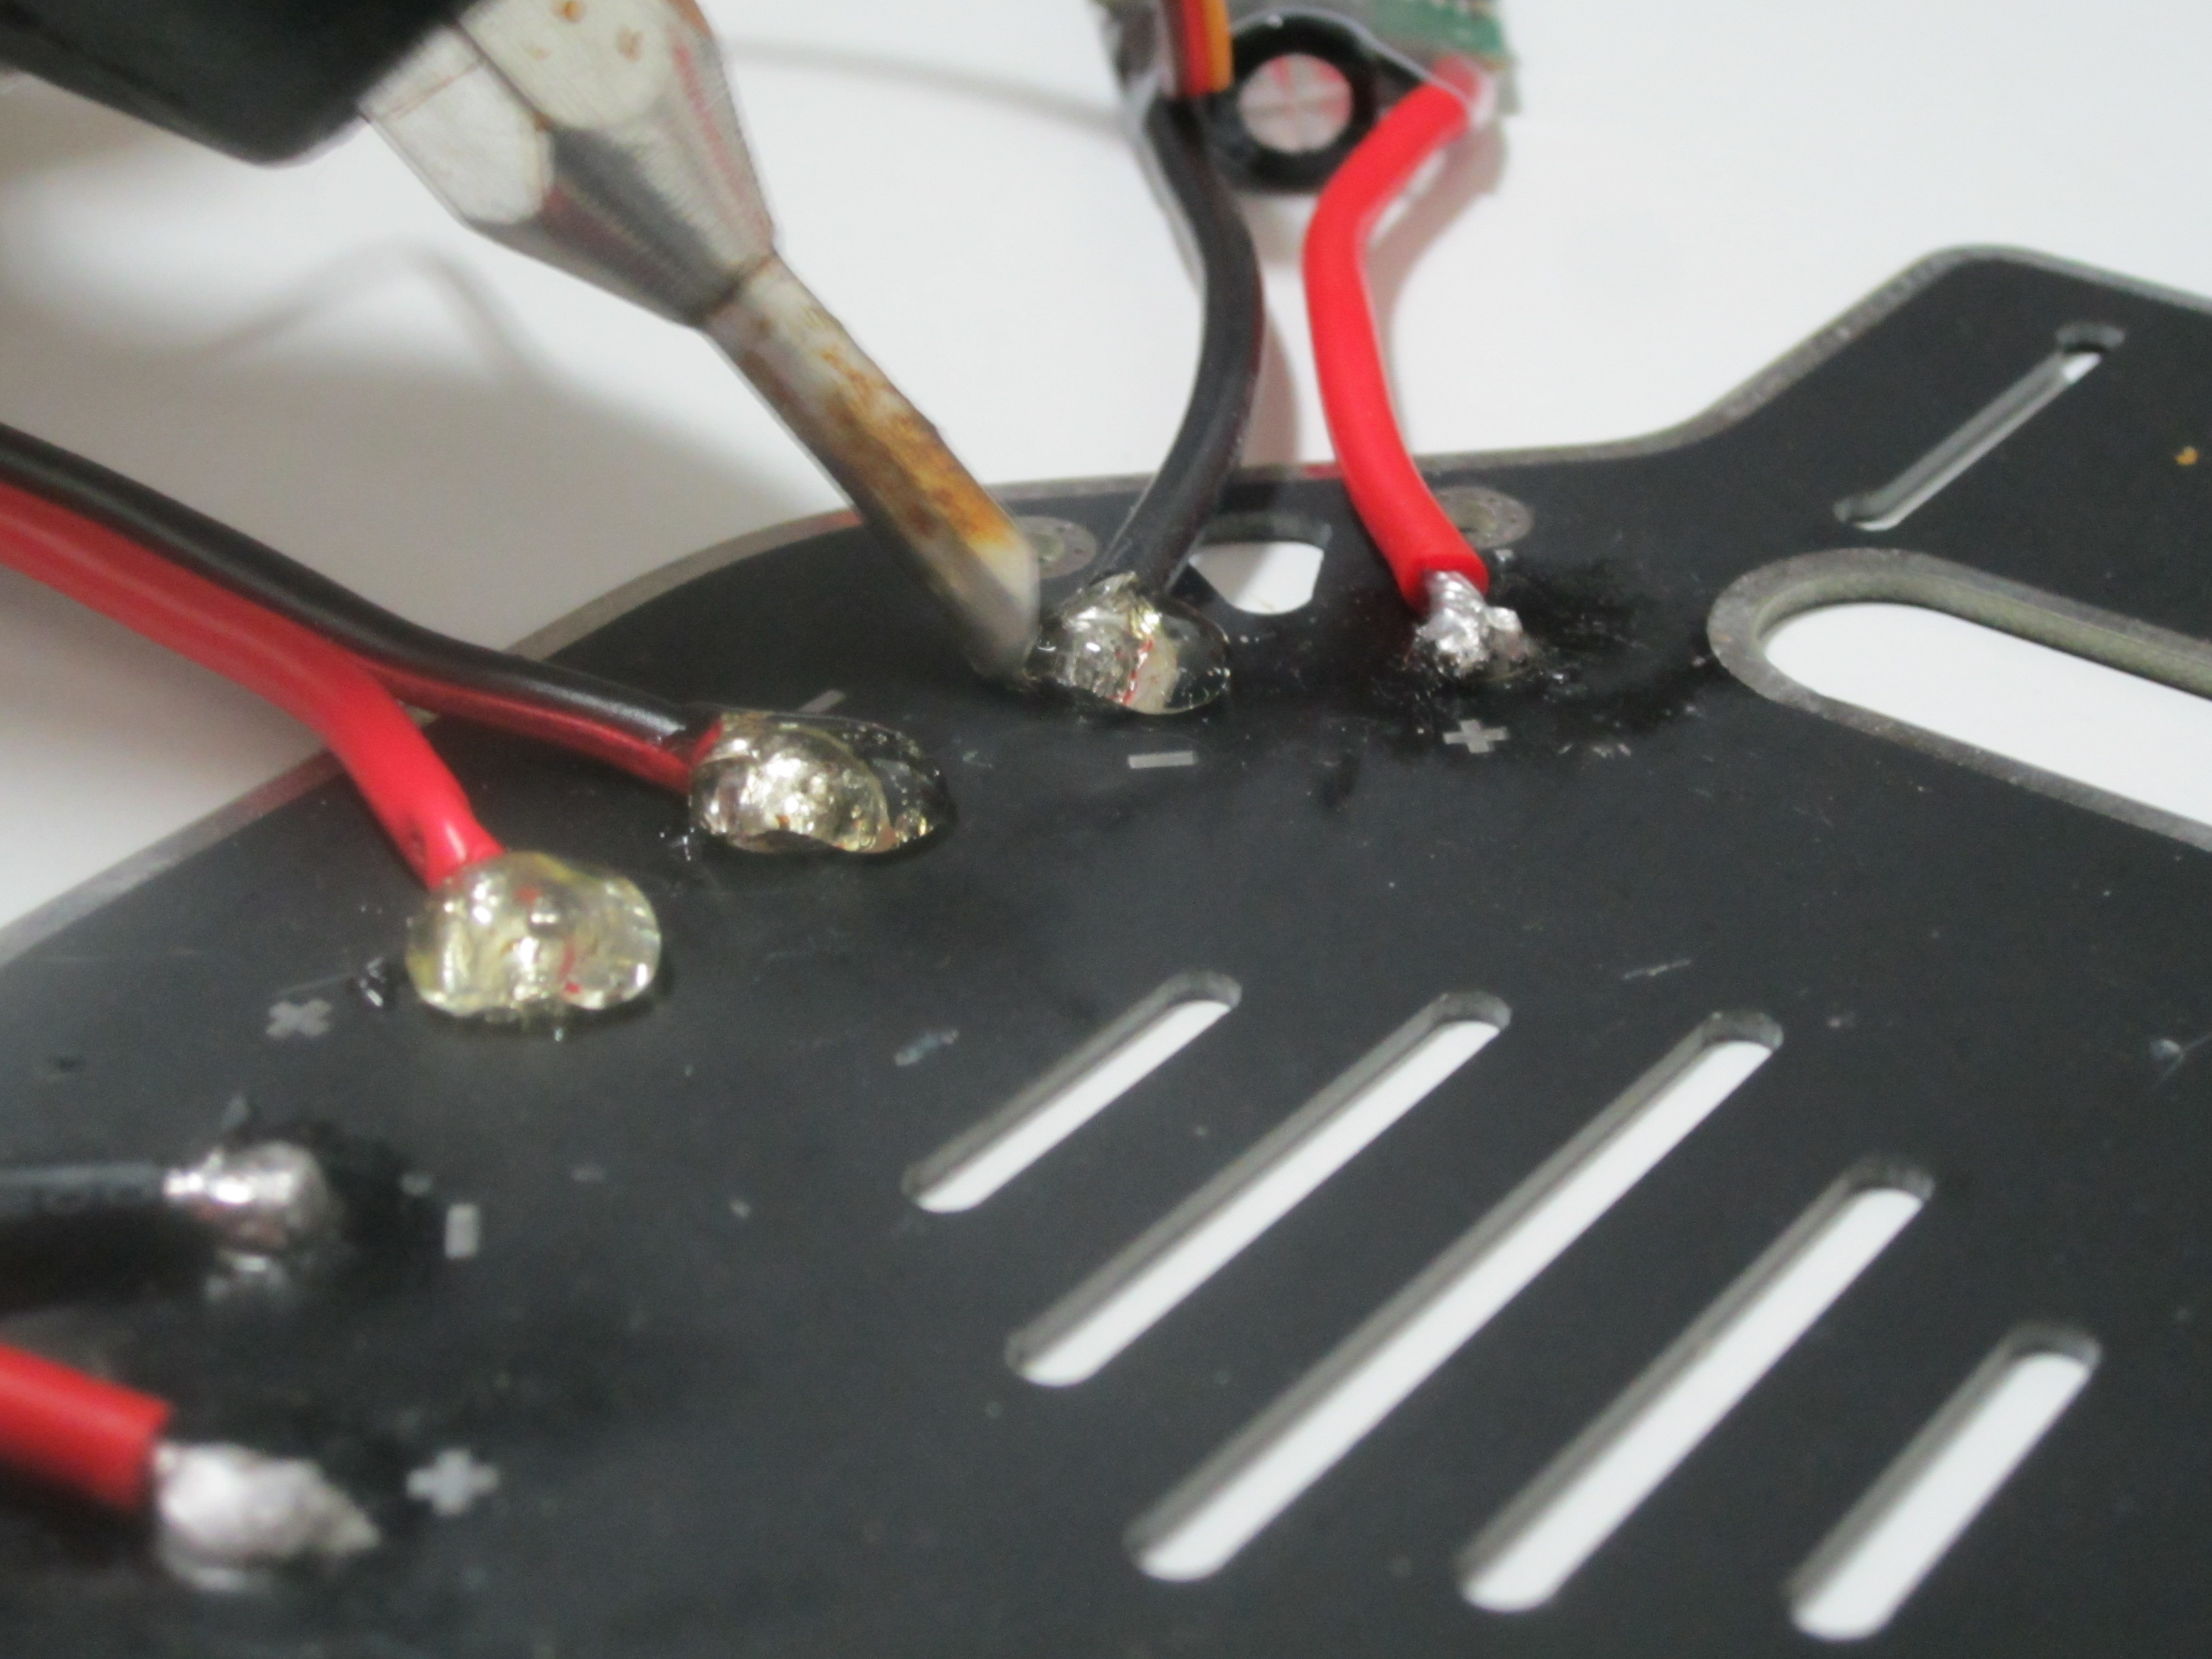
\includegraphics[width=0.8\linewidth]{Images/Mounting/IMG_0424.jpg}
  \captionof{figure}{}
  \label{fig:app1}
\end{minipage}%
\begin{minipage}{0.5\textwidth}
  \centering
  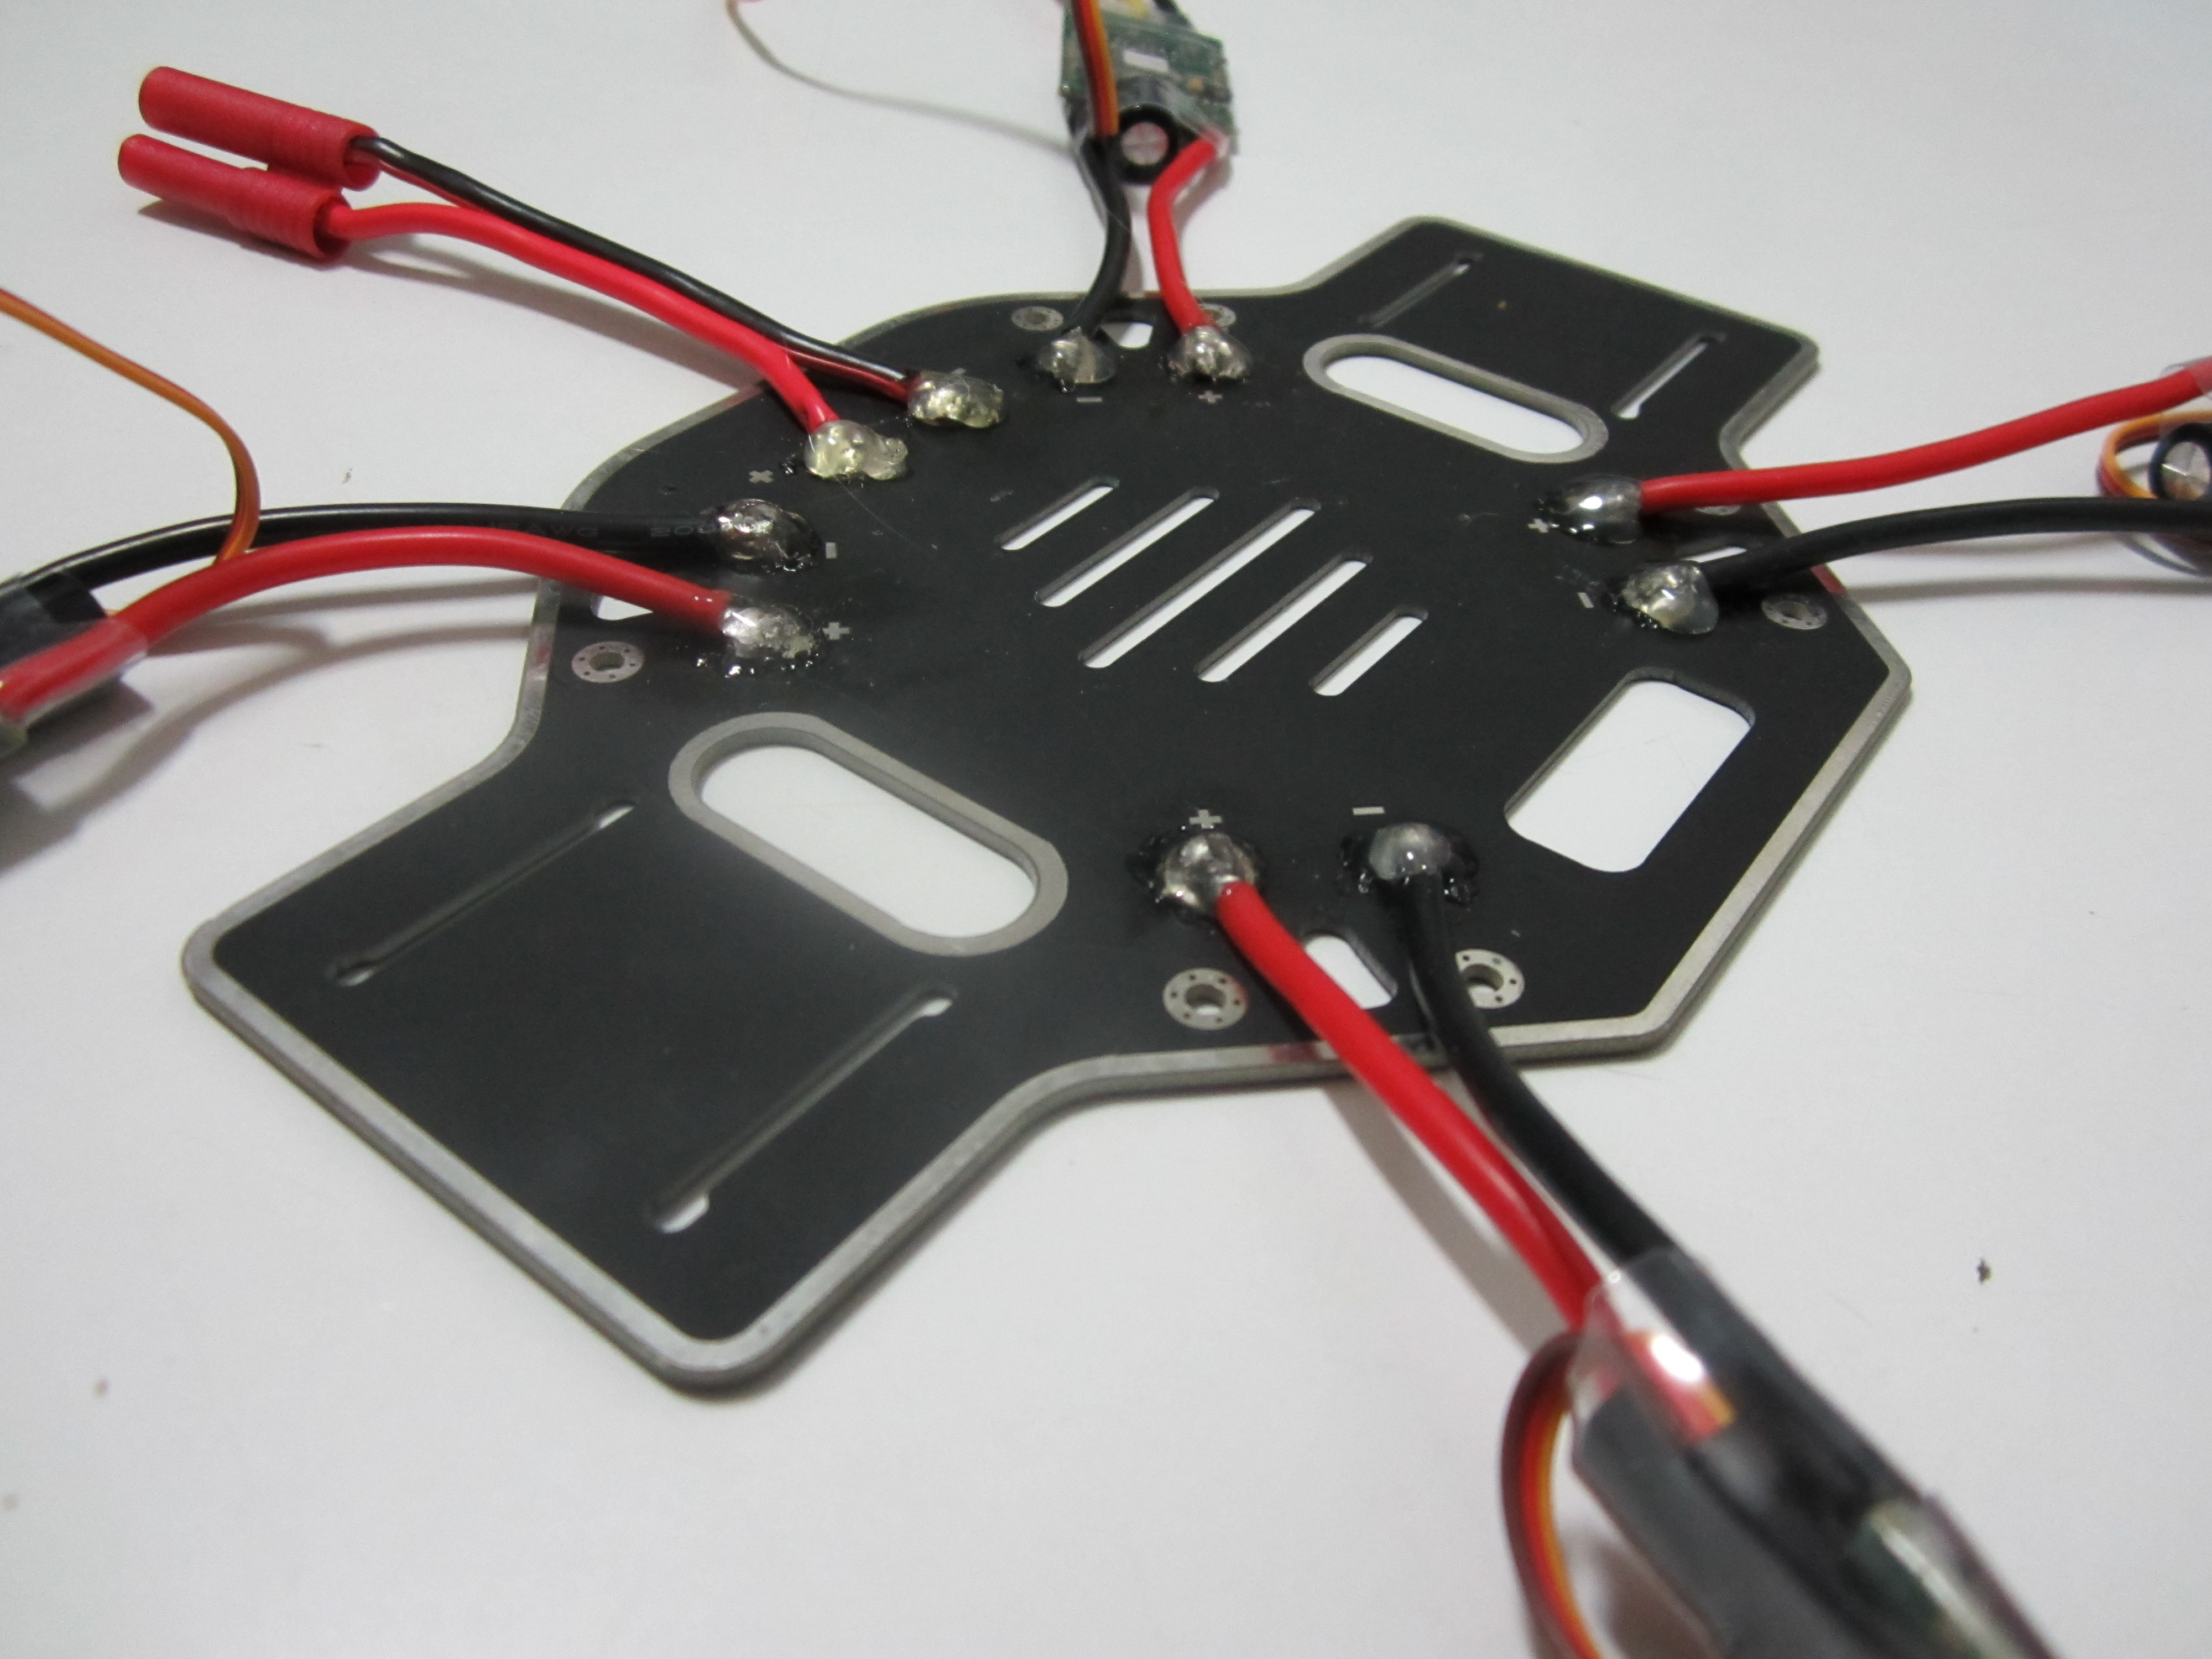
\includegraphics[width=0.8\linewidth]{Images/Mounting/IMG_0425.jpg}
  \captionof{figure}{}
  \label{fig:app2}
\end{minipage}
\\[12pt]


\section{Completion of mounting and connections}

It is important to bear in mind from now the QUAD-X figure.


%\chapter{State of the Art}

\chapter{Planning Report}

The following sections explain the tasks that I will do in the course of this project.

\section{Pieces adquisition}

This item includes the estimate time to plan which pieces are needed, how many of each, the purchase of them and the average waiting time until them arribe. 

\section{Assembling infraestructure device}

This item includes the required time to assembling the device once the pieces have arribed and we have all the needed tools.

\section{Software Implementation}

This item includes the required time to install the different software on the arduinos: the transmissor, the receptor and the controller; plus all the required software to be able to configure the arduinos through the PC.

\section{Flight Tests}

This item includes the required time to do the flight tests itself and the time to calibrate the device based on the results obtained on the tests and their interpretation.

\section{Camera incorporation}

This item includes the time needed to incorporate a camera to the device in order to take video images and transmitt it on live.

\section{Device improvements}

This item includes the required time to incorporate a bluetooth module to facilitate the connection between the arduino and the PC on a wireless mode, plus the incorporation of a GPS module, in order to extend the device possibilities.

\section{Final report}

The wording of the report is performed in parallel with the tasks that are being performed.

\section{Gantt chart}

\begin{figure}[ftbp]
  \begin{center}

    \begin{ganttchart}
    [y unit title=0.4cm, 
    y unit chart=0.5cm,
    vgrid,hgrid,
    title label anchor/.style={below=-1.6ex},
    title left shift=.05,
    title right shift=-.05,
    title height=1,
    bar/.style={fill=gray!50},
    incomplete/.style={fill=white},
    progress label text={},
    bar height=0.7,
    group right shift=0,
    group top shift=.6,
    group height=.3,
    group peaks height={}{}{.1}]{1}{24}
    
    %labels
    \gantttitle{2013-2014}{24} \\
    \gantttitle{October}{3}
    \gantttitle{November}{3} 
    \gantttitle{December}{3}
    \gantttitle{January}{3} 
    \gantttitle{February}{3} 
    \gantttitle{March}{3} 
    \gantttitle{April}{3} 
    \gantttitle{May}{3}\\
    
    %tasks
    \ganttbar{Task 1}{2}{6} \\
    \ganttbar{Task 2}{7}{12} \\
    \ganttbar{Task 3}{10}{15} \\
    \ganttbar{Task 4}{16}{24} \\
    \ganttbar{Task 5}{19}{24} \\
    \ganttbar{Task 6}{22}{24} \\
    \ganttbar{Final report}{2}{24}

    %relations 
    \ganttlink{elem0}{elem1}  
    \ganttlink{elem2}{elem3} 


   \end{ganttchart}
  \end{center}
\end{figure}




\end{document}
